\documentclass[sn-mathphys,Numbered]{sn-jnl}% Math and Physical Sciences Reference Style
%\documentclass[sn-mathphys,Numbered,draft]{sn-jnl}% Math and Physical Sciences Reference Style

%%\documentclass[sn-nature]{sn-jnl}% Style for submissions to Nature Portfolio journals
%%\documentclass[sn-basic]{sn-jnl}% Basic Springer Nature Reference Style/Chemistry Reference Style
%%\documentclass[sn-aps]{sn-jnl}% American Physical Society (APS) Reference Style
%%\documentclass[sn-vancouver,Numbered]{sn-jnl}% Vancouver Reference Style
%%\documentclass[sn-apa]{sn-jnl}% APA Reference Style 
%%\documentclass[sn-chicago]{sn-jnl}% Chicago-based Humanities Reference Style
%%\documentclass[default]{sn-jnl}% Default
%%\documentclass[default,iicol]{sn-jnl}% Default with double column layout

%%%% Standard Packages
%%<additional latex packages, if required can be included here>

\setlength{\parskip}{\baselineskip}

\usepackage{graphicx}%
\usepackage{amsmath,amssymb,amsfonts,bm}%
\usepackage{multirow}
\usepackage{amsthm}%
%\usepackage{subcaption}
\usepackage{mathrsfs}%
\usepackage[title]{appendix}%
\usepackage{xcolor}%
\usepackage{textcomp}%
\usepackage{manyfoot}%
\usepackage{booktabs}%
%\usepackage{algorithm}%
%\usepackage{algorithmicx}%
\usepackage{algpseudocode}%
\usepackage{listings}%
\usepackage{bigints}
\usepackage{outlines}
\usepackage{geometry}
\usepackage{subfigure}
\usepackage{siunitx}
\usepackage{float}
\usepackage{comment}

\geometry
{
a4paper,         % or letterpaper
textwidth=15cm,  % llncs has 12.2cm
textheight=24cm, % llncs has 19.3cm
% heightrounded,   % integer number of lines
% hratio=1:1,      % horizontally centered
% vratio=2:3,      % not vertically centered
}
\setlength{\tabcolsep}{0.5cm}
\usepackage[onehalfspacing]{setspace}
% \usepackage{lineno}
% \linenumbers
%%%%

\usepackage[utf8]{inputenc}
\usepackage{graphicx}
\usepackage[ruled,vlined]{algorithm2e}
\usepackage{amsmath}
%\usepackage{movie15} %to allow movie embedding
\usepackage[section]{placeins}
\usepackage{enumitem}
\usepackage{color,soul}
\usepackage{xfrac}

%% New math commands
\newcommand{\s}[1]{\overset{*}{#1}}
\newcommand{\RM}{\bm{\Lambda}}
\newcommand{\RMI}{\bm{\Lambda}_0}
\newcommand{\RMT}{\bm{\Lambda}_t}
\newcommand{\RV}{\bm{\psi}}
\newcommand{\magRV}{\psi}
\newcommand{\RMTS}{\s{\bm{\Lambda}}_t}
\newcommand{\bb}{\boldsymbol}
\usepackage{nicefrac}
%\usepackage{tikz}
%\usepackage{tikz-3dplot}
\usepackage{mathtools}

%% For contact
\newcommand{\rbar}{\bar{\bm{r}}}
\newcommand{\xibar}{\bar{\xi}}
%\newcommand{\magRV}{\bbit{\psi}}
\newcommand{\diag}{\rm diag}

%% Author notes for drafting (remove before submission).
%% \todo{...}     conspicuous block note; breaks across pages
%% \citetodo{...} placeholder for a citation not yet in bibliography.bib
\newcommand{\todo}[1]{\par\noindent\textcolor{red}{\rule{\linewidth}{0.8pt}}\par\nopagebreak
	\noindent{\small\color{red!70!black}\textbf{AUTHOR NOTE:} #1\par}\nopagebreak
	\noindent\textcolor{red}{\rule{\linewidth}{0.8pt}}\par}
\newcommand{\citetodo}[1]{\textcolor{red}{[\textbf{cite:}~#1]}}

%% Supplement toggle. false (default): the FEBio ring comparison is Appendix B of this file.
%% true: it is only in the standalone supplement_febio_ring.tex (Sec. S1, Figs. S1-S2) and
%% Appendix B is omitted here. See supplement_febio_ring.tex for the build command.
\newif\ifsupplementseparate
\supplementseparatefalse
%\supplementseparatetrue
\ifsupplementseparate
  \newcommand{\suppRef}{the Supplementary Material, Sec.~S1}
  \newcommand{\suppFigDecay}{Figure~S1 of the Supplementary Material}
  \newcommand{\suppFigBoth}{Figures~S1 and~S2}
\else
  \newcommand{\suppRef}{Appendix~\ref{app:ring_febio}}
  \newcommand{\suppFigDecay}{Figure~\ref{fig:ring_febio_decay} of Appendix~\ref{app:ring_febio}}
  \newcommand{\suppFigBoth}{Figures~\ref{fig:ring_febio_decay} and~\ref{fig:ring_febio_traction}}
\fi

\begin{document}

\title[Verification benchmarks for fluid--solid interaction]{Benchmark problems are not benchmark solutions: an open verification suite for continuum fluid--solid interaction with quantified numerical uncertainty}

\author*[1]{\fnm{Philip} \sur{Cardiff}}\email{philip.cardiff@ucd.ie}
%\author*[1,2,3]{\fnm{Philip} \sur{Cardiff}}\email{philip.cardiff@ucd.ie}
%\author[1,2,3]{\fnm{Dylan} \sur{Armfield}}
%%\author[5]{\fnm{Hiroaki} \sur{Nishikawa}}
%\author[4]{\fnm{\v{Z}eljko} \sur{Tukovi\'{c}}}
\author[3]{\fnm{Emad} \sur{Tandis}}
% ORCID 0000-0002-2409-7332 (https://orcid.org/0000-0002-2409-7332): not typeset because sn-jnl.cls \orcid needs Orcidlogo.eps, which is not in the repository.
\author[1]{\fnm{Sairam} \sur{Pamulaparthi Venkata}}
% Ivan Batisti\'{c} stays the final (senior) author: add any further authors above this line.
\author[1,2]{\fnm{Ivan} \sur{Batisti\'{c}}}

\affil[1]{\orgdiv{School of Mechanical and Materials Engineering}, \orgname{University College Dublin}, \orgaddress{\country{Ireland}}}
%\affil[2]{\orgdiv{UCD Centre for Mechanics}, \orgname{University College Dublin}, \orgaddress{\country{Ireland}}}
%\affil[3]{\orgdiv{I-Form Centre}, \orgname{University College Dublin}, \orgaddress{\country{Ireland}}}
\affil[2]{\orgdiv{Faculty of Mechanical Engineering and Naval Architecture}, \orgname{University of Zagreb}, \orgaddress{\country{Croatia}}}
\affil[3]{\orgname{Aston University}, \orgaddress{\city{Birmingham}, \country{United Kingdom}}}% TODO: add the school/department
%\affil[5]{\orgname{National Institute of Aerospace}, \orgaddress{\country{Hampton, VA 23666, USA}}}



\abstract{
Many benchmark problems exist for fluid--solid interaction (FSI), but few benchmark solutions come with a rigorously established numerical uncertainty, and agreement with a published value is often taken as evidence that a code is correct.
This paper assembles an open, executable verification suite for continuum FSI and classifies each reference by its quality: analytical (A), independently converged numerical with at most a small, quantified model-form difference (B), published but incompletely quantified (C), and weak (C-weak).
For each benchmark the spatial, temporal and iterative errors are studied separately and the quantities of interest are reported with their observed convergence behaviour; verification against the mathematical problem is kept separate from validation against experiment.
All calculations use the partitioned finite volume FSI framework of the open-source toolbox solids4foam: a PIMPLE-type arbitrary Lagrangian--Eulerian fluid, small-strain and total Lagrangian solids of standard and high-order accuracy, and Dirichlet--Neumann (Aitken, IQN-ILS) or Robin--Neumann coupling.
For two analytical problems (an added-mass ring and a thick-walled Womersley tube) and an independently computed collapsible channel, most quantities converge at observed orders close to the nominal two, and the finest solutions agree with the references to within the reference uncertainty or a small identified error.
The widely used benchmarks are less conclusive.
For the Hron--Turek FSI3 problem, a two-level agreement with the Featflow reference disappears on a third level: with the tutorial set-up the displacements converge at an observed order of about one. This was traced to a path-dependent mesh motion and a first-order wall-pressure condition. With these corrected, the large changes between levels disappear, but a fourth level ($7.5\times10^5$ fluid cells) shows that the displacements are still not in the asymptotic range: they change by 1--2\% from the third level, towards the reference, and differ from it by 2\% ($u_y$) and 4.5\% ($u_x$), while the reference itself changes by up to 4\% between its two finest levels.
For a three-dimensional pressure-pulse tube, verification exposed two solver defects, a compiler-dependent aliasing error and a mesh-dependent degeneracy of the interface interpolation, and showed that much of a 20--25\% discrepancy between published solutions is reproduced by the difference in time integration.
A third finding concerns the iterative error: a widely used form of the coupling convergence test can accept unconverged steps in slowly varying phases, producing a drift that a steadiness check on the quantity of interest does not detect.
The suite, its drivers and its machine-readable references are released so that verification claims can be re-executed rather than accepted on trust.
}

\keywords{Fluid--solid interaction, Code verification, Benchmark, Reference solution, Numerical uncertainty, Partitioned coupling, Finite volume method, solids4foam, OpenFOAM}

\maketitle

\todo{Title, abstract, Introduction and Section~\ref{sec:numerical_methods} rewritten (October 2026) around the partitioned solution procedures that produced every result. Section~\ref{sec:math_model} is that of the parent paper, amended (October 2026) for the displacement-based partitioned solids and the small-strain formulation; its notation should remain consistent with the companion solver paper. Abstract numbers must be re-checked against Sections~\ref{sec:benchmark_suite}--\ref{sec:cross_benchmark} before submission.}


%%%%%%%%%%%%%%%%%%%%%%%%%%%%%%%%%%%%%%%%%%%%%%%%%%%%%%%%%%%%%%%%%%
%%%%%%%%%%%%%%%%%%%%%%%%%%%%%%%%%%%%%%%%%%%%%%%%%%%%%%%%%%%%%
\section{Introduction}\label{sec:intro}
%%%%%%%%%%%%%%%%%%%%%%%%%%%%%%%%%%%%%%%%%%%%%%%%%%%%%%%%%%%%%
Benchmark problems are central to the development of fluid--solid interaction (FSI) codes: they are used to demonstrate accuracy, to compare coupling algorithms and to support claims that a new method is correct.
Many such problems exist, from the flag-behind-a-cylinder family of \citet{Turek2006} to pressure-pulse tubes, lid-driven cavities with flexible membranes and three-dimensional flows past elastic plates.
Far fewer of them come with a benchmark \emph{solution} whose own numerical error has been established: published values are often single-mesh results, are read from figures, are reported without time-step studies, or differ between sources by more than the discretisation errors that they are used to judge.
Agreement with such a value is then weak evidence, and disagreement is ambiguous: it may mean that the code under test is wrong, that the reference is wrong, or that the code's own solution is not yet resolved.
This paper addresses that gap for continuum FSI with an open, executable verification suite in which the quality of every reference and the spatial, temporal and iterative errors of every result are stated explicitly.

FSI formulations differ in how the fluid and solid are described (Eulerian, Lagrangian, or an arbitrary Lagrangian--Eulerian (ALE) fluid with a Lagrangian solid), in whether the interface conditions are satisfied at every time step (strong coupling) or only approximately (weak coupling), and in whether the fields are solved separately or as one system (partitioned or monolithic); the companion solver paper~\citep{CardiffBatistic2026QM} reviews these choices.
The present work concerns strongly coupled FSI with a body-fitted ALE fluid and a Lagrangian solid, solved by partitioned finite volume procedures in which separate field solvers are iterated at each time step until the interface conditions are met.
Weakly coupled schemes are not considered, as they become unstable when the added mass of the fluid is large relative to the inertia of the solid~\citep{Causin2005, Forster2006}.

The verification literature for FSI is smaller than that for its component fields.
The proposal of \citet{Turek2006} defines the most widely used problems and reports multi-level reference values, and goal-oriented error estimation has been developed for FSI in the finite element setting~\citep{Richter2012, Richter2017}; monolithic finite element and hybrid finite volume/finite element codes have been demonstrated on these and related problems~\citep{Heil2004, Heil2008, Eken2016, Lozovskiy2019}, with convergence evidence that ranges from multi-level studies to single-mesh results.
Partitioned finite volume FSI, including the OpenFOAM-based framework of \citet{Tukovic2018} on which the solids4foam toolbox~\citep{Cardiff2025} builds, has mostly been assessed by comparison with such published values.
Across this literature, the error of the reference itself is rarely quantified, iterative (coupling) errors are seldom separated from discretisation errors, and the time integration of a reference is often first order with a large step, so that two codes can disagree because their references differ rather than because either is wrong.
General verification practice --- observed orders from systematic refinement, separation of error sources, and the distinction between verification and validation~\citep{Roache1998, Oberkampf2010} --- is well established for single-field problems but is applied unevenly to coupled FSI.

The present work applies that practice to a suite of continuum FSI benchmarks, all solved with one partitioned, cell-centred finite volume framework: a PIMPLE-type ALE fluid, small-strain and total Lagrangian finite volume solids with standard and high-order discretisations~\citep{Cardiff2026, Batistic2026}, and Dirichlet--Neumann (Aitken~\citep{kuttler2008fixed}, IQN-ILS~\citep{Degroote2009}) or Robin--Neumann~\citep{Tukovic2018b} coupling.
The aim is not to promote a solver but to establish, case by case, what the available references can and cannot verify, and how much of the remaining difference is attributable to the code under test.
Verification here means convergence of the discrete solution to the solution of the stated mathematical problem; agreement with experimental data is validation, is kept separate, and is never used as evidence of convergence.

The specific contributions are:
\begin{enumerate}
    \item A reference-quality classification for FSI benchmarks (category A: analytical; B: independently converged numerical solution, possibly of a problem with a small, quantified model-form difference; C: published values with incompletely quantified error; C-weak: digitised, single-mesh, inconsistent or same-lineage values), applied to every case in the suite.
    \item Spatial, temporal and iterative error studies for each benchmark, with observed orders reported only where the evidence supports them, and with the slowest-converging quantity of interest identified.
    \item Evidence that verification exposes real defects and misleading benchmark agreement: two solver defects found through a cross-platform discrepancy in a three-dimensional tube, one compiler-dependent and one that changed the interface interpolation with mesh level; a two-level agreement with the Hron--Turek FSI3 reference that disappears on a third level; a published code-to-code discrepancy that is largely reproduced by the difference in time integration; and a default coupling convergence test that can accept unconverged steps.
    \item An open, executable implementation of the suite in solids4foam~\citep{Cardiff2025}: case set-ups, verification drivers that compute the quantities of interest and observed orders, and machine-readable reference files with their provenance, so that the studies can be re-run on other codes and platforms.
\end{enumerate}

Section~\ref{sec:math_model} states the governing equations and Section~\ref{sec:numerical_methods} the partitioned finite volume procedures used for every result.
Section~\ref{sec:verification_methodology} sets out the verification methodology, Section~\ref{sec:benchmark_suite} presents the benchmark suite, Section~\ref{sec:cross_benchmark} draws cross-benchmark conclusions, and Section~\ref{sec:recommended_suite} proposes a recommended verification suite.
Section~\ref{sec:discussion} discusses the findings and Section~\ref{sec:conclusion} concludes.
\hl{Before submission, verify all references have correct details}

%%%%%%%%%%%%%%%%%%%%%%%%%%%%%%%%%%%%%%%%%%%%%%%%%%%%%%%%%%%%%%%%%%

%%%%%%%%%%%%%%%%%%%%%%%%%%%%%%%%%%%%%%%%%%%%%%%%%%%%%%%%%%%%%%%%%%
%%%%%%%%%%%%%%%%%%%%%%%%%%%%%%%%%%%%%%%%%%%%%%%%%%%%%%%%%%%%%
\section{Mathematical Models}\label{sec:math_model}
%%%%%%%%%%%%%%%%%%%%%%%%%%%%%%%%%%%%%%%%%%%%%%%%%%%%%%%%%%%%%
% Rewritten 1 Nov 2026 (overlap split with the companion solver paper):
% same model and notation, condensed, displacement-based solid only.

Every benchmark couples an incompressible Newtonian fluid to an elastic solid.
The fluid occupies $\Omega_F(t)$ and the solid $\Omega_S(t)$, and they meet on the interface $\Gamma_\text{fsi}(t) = \partial\Omega_F(t) \cap \partial\Omega_S(t)$; $\hat{\bb{n}}_F$ and $\hat{\bb{n}}_S$ are the outward unit normals of the two regions, so that $\hat{\bb{n}}_F = -\hat{\bb{n}}_S$ on $\Gamma_\text{fsi}$.
Subscripts $F$ and $S$ mark the region and are dropped where the region is clear, and a subscript $0$ marks the initial configuration.
Following OpenFOAM, the gradient of a vector is $(\bb{\nabla}\bb{a})_{ij} = \partial a_j/\partial x_i$, the transpose of the usual continuum-mechanics convention, and $\bb{\nabla}_0$ differentiates with respect to the initial coordinates.
Body forces are per unit mass.

%%--------------------------------------------------------------------------------------------------------------------%%
\subsection{Solid model} \label{sec:solid_model}
%%--------------------------------------------------------------------------------------------------------------------%%

The solid is described in total Lagrangian form with the displacement $\bb{D}_S$ from the initial configuration $\Omega_{S,0}$ as the unknown.
With the deformation gradient $\bb{F} = \bb{I} + (\bb{\nabla}_0 \bb{D}_S)^T$, $J = \det\bb{F}$, and the first Piola--Kirchhoff stress $\bb{P}_S = J\bb{\sigma}_S\bb{F}^{-T}$, where $\bb{\sigma}_S$ is the Cauchy stress, the balance of linear momentum over any part of the initial configuration reads
\begin{equation}
    \int_{\Omega_{S,0}} \rho_{S,0} \frac{\partial^2 \bb{D}_S}{\partial t^2} \, \text{d}\Omega_{S,0}
    =
    \oint_{\Gamma_{S,0}} \hat{\bb{n}}_{S,0} \cdot \bb{P}_S^T \, \text{d}\Gamma_{S,0}
    +
    \int_{\Omega_{S,0}} \rho_{S,0} \bb{b}_S \, \text{d}\Omega_{S,0},
    \label{eqn:solid_momentum_TL}
\end{equation}
with the time derivative taken at fixed material coordinates, so that $\bb{v}_S = \partial\bb{D}_S/\partial t$.
The stress comes from linear elasticity or from a neo-Hookean or Saint Venant--Kirchhoff hyperelastic law.
Where the strains and rotations are small, the geometrically linear form is used instead: $\bb{F} \approx \bb{I}$ and $\bb{P}_S \approx \bb{\sigma}_S$ in Equation~\eqref{eqn:solid_momentum_TL}, with Hooke's law and Lam\'e parameters $\mu_S$ and $\lambda_S$.
The solid boundaries carry prescribed displacements, prescribed tractions or symmetry conditions, besides the interface conditions of Section~\ref{sec:fsi_interface}.

%%--------------------------------------------------------------------------------------------------------------------%%
\subsection{Fluid model}
\label{sec:fluid_governing_eqn}
%%--------------------------------------------------------------------------------------------------------------------%%

The fluid is laminar, isothermal, incompressible and Newtonian, and is described on the moving domain $\Omega_F(t)$ in arbitrary Lagrangian--Eulerian (ALE) form, with $\bb{v}^\Gamma$ the velocity of the domain.
The domain follows the solid on $\Gamma_\text{fsi}$; inside $\Omega_F$ its motion is a numerical choice (Section~\ref{sec:fluid_mesh_motion}) that must satisfy the geometric conservation law
\begin{equation}
    \frac{d}{dt} \int_{\Omega_F} \text{d}\Omega_F - \oint_{\Gamma_F} \hat{\bb{n}}_F \cdot \bb{v}^\Gamma \, \text{d}\Gamma_F = 0 .
    \label{eqn:gcl}
\end{equation}
With Equation~\eqref{eqn:gcl}, mass conservation over a moving control volume reduces to $\oint_{\Gamma_F} \hat{\bb{n}}_F \cdot \bb{v}_F \, \text{d}\Gamma_F = 0$, and momentum conservation is
\begin{equation}
    \frac{d}{dt} \int_{\Omega_F} \bb{v}_F \, \text{d}\Omega_F
    + \oint_{\Gamma_F} \hat{\bb{n}}_F \cdot (\bb{v}_F - \bb{v}^\Gamma)\, \bb{v}_F \, \text{d}\Gamma_F
    = \oint_{\Gamma_F} \hat{\bb{n}}_F \cdot \bb{\sigma}_F^* \, \text{d}\Gamma_F
    + \int_{\Omega_F} \bb{b}_F \, \text{d}\Omega_F,
    \label{eqn:fluid_momentum_ale}
\end{equation}
with the kinematic stress $\bb{\sigma}_F^* = \nu\left[\bb{\nabla}\bb{v}_F + (\bb{\nabla}\bb{v}_F)^T\right] - p_F \bb{I}$, where $p_F$ is the kinematic pressure (pressure over density), $\nu$ the kinematic viscosity, and $\bb{\sigma}_F = \rho_F \bb{\sigma}_F^*$ the Cauchy stress.
The fluid boundaries are inlets, outlets, no-slip walls and symmetry planes; the conditions of each benchmark are those of its solids4foam tutorial.

%%--------------------------------------------------------------------------------------------------------------------%%
\subsection{Interface conditions}
\label{sec:fsi_interface}
%%--------------------------------------------------------------------------------------------------------------------%%

On $\Gamma_\text{fsi}$ the fluid sticks to the solid, which also moves the fluid domain, and the tractions balance:
\begin{equation}
    \bb{v}_F = \bb{v}^\Gamma = \frac{\partial \bb{D}_S}{\partial t},
    \qquad
    \rho_F \, \hat{\bb{n}}_F \cdot \bb{\sigma}_F^* + \hat{\bb{n}}_S \cdot \bb{\sigma}_S = \bb{0}
    \qquad \text{on } \Gamma_\text{fsi}(t).
    \label{eqn:kinematic_interface}
\end{equation}
With consistent initial conditions, the kinematic condition keeps the interface free of gaps and overlaps.

%%%%%%%%%%%%%%%%%%%%%%%%%%%%%%%%%%%%%%%%%%%%%%%%%%%%%%%%%%%%%%%%%%


%%%%%%%%%%%%%%%%%%%%%%%%%%%%%%%%%%%%%%%%%%%%%%%%%%%%%%%%%%%%%%%%%%
%%%%%%%%%%%%%%%%%%%%%%%%%%%%%%%%%%%%%%%%%%%%%%%%%%%%%%%%%%%%%
\section{Numerical methods}\label{sec:numerical_methods}
%%%%%%%%%%%%%%%%%%%%%%%%%%%%%%%%%%%%%%%%%%%%%%%%%%%%%%%%%%%%%
% Every result in Sections 4-6 was produced with the partitioned procedures
% described here (solids4foam fluidSolidInterface: fixedRelaxation, Aitken,
% IQNILS; Robin condition elasticWallPressure). The experimental
% quasi-monolithic solver of the parent paper is not used; its description is
% preserved, outside the build, in sectionNumericalModelQuasiMonolithic.tex.
% Source checked: solids4foam development (src/solids4FoamModels:
% fluidModels/pimpleFluid, solidModels, fluidSolidInterfaces) and the case
% dictionaries of the tutorials in Section 5.

All results in this paper were obtained with the partitioned fluid--solid interaction framework of the open-source toolbox solids4foam~\citep{Cardiff2025}, which builds on the OpenFOAM finite volume library~\citep{Weller1998} and follows the partitioned approach of \citet{Tukovic2018}.
The fluid and the solid are discretised on separate cell-centred finite volume meshes and solved by separate field solvers, which exchange interface displacements and tractions within each time step.
This section summarises the components that determine the discretisation, temporal and iterative errors studied in Sections~\ref{sec:verification_methodology}--\ref{sec:cross_benchmark}; implementation detail is in the solids4foam source and in the case dictionaries that accompany each benchmark.
Case-specific choices (time scheme, convection scheme, solid variant, coupling algorithm and tolerances) are stated with each benchmark in Section~\ref{sec:benchmark_suite}.

%%--------------------------------------------------------------------------------------------------------------------%%
\subsection{Fluid}\label{sec:fluid_solver}
%%--------------------------------------------------------------------------------------------------------------------%%

The incompressible Navier--Stokes equations in ALE form (Section~\ref{sec:fluid_governing_eqn}) are solved by the \texttt{pimpleFluid} model, a solids4foam port of the OpenFOAM \texttt{pimpleFoam} solver.
Velocity and pressure are collocated at cell centres; the face fluxes are obtained by Rhie--Chow-type momentum interpolation~\citep{Rhie1983}, and the pressure--velocity coupling is the segregated PIMPLE algorithm (PISO pressure correctors within SIMPLE-type outer correctors), with the numbers of outer and pressure correctors stated per case.
Spatial operators are the standard second-order finite volume operators: midpoint quadrature, linear face interpolation, least-squares or Gauss cell gradients, and Laplacian face fluxes with explicit non-orthogonal correction~\citep{Jasak1996}.
Convection is discretised with central (\texttt{linear}) or limited linear-upwind interpolation, depending on the case.
The time derivative is discretised with the second-order backward difference formula (BDF2, \texttt{backward}) unless stated; implicit Euler is used only in the deliberate time-scheme comparison of Section~\ref{sec:3dtube}.
On the moving mesh the convective flux is the relative flux $\bb{\Gamma}_f\cdot(\bb{v}_f - \bb{v}^\Gamma_f)$, where the mesh flux $\bb{\Gamma}_f\cdot\bb{v}^\Gamma_f$ is the volume swept by face $f$.
With BDF2 the swept volumes of the last two steps are combined with the BDF2 weights, so that the discrete space-conservation law (Equation~\eqref{eqn:gcl}) holds for the backward volume derivative.
On the interface the fluid velocity equals the velocity of the moving wall, and the interface traction passed to the solid is the sum of the pressure and viscous tractions on the fluid interface faces.

\subsection{Fluid mesh motion}\label{sec:fluid_mesh_motion}

The interior fluid mesh follows the interface through a Laplacian equation for the cell motion velocity (\texttt{velocityLaplacian}), whose diffusivity varies with the inverse (in most cases the inverse square) of the distance to the moving boundaries, so that cells near the interface move almost rigidly~\citep{Tukovic2018}.
The interface displacement is the solid displacement transferred to the fluid interface (Section~\ref{sec:interface_transfer}); the point motion is obtained from the cell motion velocity by interpolation, and the mesh points are moved once per coupling iteration.
Mesh motion is a numerical device: it changes the discrete solution only through the mesh quality and through the space-conservation and moving-wall treatments described above.

%%--------------------------------------------------------------------------------------------------------------------%%
\subsection{Solid}\label{sec:solid_solver}
%%--------------------------------------------------------------------------------------------------------------------%%

The solid momentum equation (Section~\ref{sec:solid_model}) is discretised by a cell-centred finite volume method with the total displacement as unknown~\citep{Jasak2000, Cardiff2021}.
Two kinematic formulations are used: a small-strain (linear geometry) formulation for the linear-elastic walls (ringAddedMass, womersleyTube, 3dTube), and a total Lagrangian formulation for the finite-strain problems, with St Venant--Kirchhoff (Hron--Turek, collapsibleChannel, mokLidDrivenCavity) or neo-Hookean (Hessenthaler) material laws.
The time derivative uses BDF2, and each solid solve is a Newton--Krylov iteration through the PETSc SNES interface~\citep{PETSc, Cardiff2026}.
Two spatial variants are used.
The \emph{standard} variant uses a linear least-squares reconstruction of the displacement and a compact-stencil momentum stabilisation, a Rhie--Chow-type difference between the compact and the reconstructed face normal gradient, scaled by a user factor~\citep{Cardiff2026}; it is formally second order, but the stabilisation is not negligible on coarse meshes and stiffens thin, bending-dominated structures (Section~\ref{sec:fsi1}).
The \emph{high-order} variant evaluates the face fluxes of the residual from a cubic moving-least-squares reconstruction of the displacement~\citep{Batistic2026}.
Which variant is used is stated per case, because for thin bending-dominated walls the choice can dominate the coupled error (Section~\ref{sec:collapsible}).

%%--------------------------------------------------------------------------------------------------------------------%%
\subsection{Interface transfer}\label{sec:interface_transfer}
%%--------------------------------------------------------------------------------------------------------------------%%

Displacements are transferred from the solid to the fluid interface at the interface points, and tractions from the fluid to the solid interface at the faces.
Where the two interface meshes coincide (ringAddedMass, womersleyTube, collapsibleChannel, mokLidDrivenCavity), a direct one-to-one map is used.
Where they do not (Hron--Turek, 3dTube, Hessenthaler), face tractions are interpolated with arbitrary-mesh-interface (AMI) weights, and point displacements by barycentric interpolation on a triangulation of the donor interface faces.
The interface transfer is part of the discretisation: it is an operator that must converge with refinement like any other, and in 3dTube a defect in it changed with mesh level (Section~\ref{sec:3dtube}).

%%--------------------------------------------------------------------------------------------------------------------%%
\subsection{Coupling algorithms}\label{sec:coupling_algorithms}
%%--------------------------------------------------------------------------------------------------------------------%%

Strong coupling is enforced by outer (coupling) iterations within each time step.
Two interface formulations are used.

\paragraph{Dirichlet--Neumann.}
The fluid receives the interface displacement (mesh motion and wall velocity) and the solid receives the fluid traction.
Each time step starts with a solid predictor, i.e.\ a solid solve with the fluid traction of the previous step, whose displacement is passed to the fluid without relaxation in the first iteration~\citep{Tukovic2018}.
Subsequent interface displacements are updated by fixed under-relaxation, by Aitken dynamic relaxation~\citep{kuttler2008fixed}, or by the interface quasi-Newton inverse least-squares method (IQN-ILS)~\citep{Degroote2009}, which builds an approximate inverse Jacobian of the interface residual from the secant information of the current and, optionally, previous time steps; secant columns that are repeated or nearly linearly dependent are filtered before the least-squares solve.

\paragraph{Robin--Neumann.}
The fluid pressure satisfies a Robin condition on the interface that accounts for the solid inertia through an estimate $\rho_S h_S$ of the solid interface impedance~\citep{Tukovic2018b}, and the iterations are unrelaxed fixed-point iterations.
The Robin condition modifies the discrete interface condition within the iterations; at convergence the interface flux is made consistent with the mesh motion.
Because it changes the iteration rather than only accelerating it, the converged Robin--Neumann and Dirichlet--Neumann solutions need not agree to the coupling tolerance (Section~\ref{sec:ref_hierarchy}).

\paragraph{Convergence test.}
The interface residual $\bb{r}$ is the difference between the solid interface point positions, transferred to the fluid interface, and the fluid interface point positions.
Two normalised measures are formed,
\begin{equation}
	r_1 = \frac{\|\bb{r}\|}{\max_k \|\bb{r}^{(k)}\|},
	\qquad
	r_2 = \frac{\|\bb{r}\|}{\|\bb{d}^\Gamma\|_{\max}},
	\label{eq:coupling_residuals}
\end{equation}
where the maximum in $r_1$ is over the coupling iterations $k$ of the current step and $\|\bb{d}^\Gamma\|_{\max}$ is the largest norm of the \emph{total} interface displacement seen so far.
In the legacy default a step is accepted when $\min(r_1, r_2)$ is below the coupling tolerance; a strict option requires $\max(r_1, r_2)$ to be below it.
The two tests differ greatly in slowly varying phases with a large total interface displacement, where $r_2$ can be small after a single relaxed iteration whatever the reduction of the residual within the step (Section~\ref{sec:iterative_errors}).
Robin--Neumann iterations additionally require the change of interface pressure and the interface leakage flux to fall below their own tolerances.
By default, a step that does not meet the test within the maximum number of iterations stops the run; the default test can nevertheless accept insufficiently converged steps, as shown in Section~\ref{sec:iterative_errors}.

%%--------------------------------------------------------------------------------------------------------------------%%
\subsection{Solution procedure and toolchain}\label{sec:implementation_details}
%%--------------------------------------------------------------------------------------------------------------------%%

The partitioned procedure for one time step is summarised in Algorithm~\ref{alg:partitioned_fsi}.

\begin{algorithm}[htbp]
\caption{Partitioned FSI procedure for one time step (solids4foam \texttt{fluidSolidInterface}).}
\label{alg:partitioned_fsi}
\begin{algorithmic}[1]
\State Advance time; solve the solid with the fluid traction of the previous step (predictor).
\State Transfer the predicted interface displacement to the fluid interface.
\State For coupling iterations $k = 1, 2, \ldots$, up to the maximum number:
\State \hspace{1.5em}move the fluid mesh to the current interface displacement and update the mesh fluxes;
\State \hspace{1.5em}solve the fluid (PIMPLE outer and pressure correctors) with the moving-wall velocity, or with the Robin pressure condition;
\State \hspace{1.5em}transfer the fluid interface traction to the solid and solve the solid (Newton--Krylov);
\State \hspace{1.5em}transfer the solid interface displacement to the fluid interface and evaluate $\bb{r}$, $r_1$ and $r_2$;
\State \hspace{1.5em}stop if the convergence test (and, for Robin--Neumann, the pressure and flux tests) is met;
\State \hspace{1.5em}otherwise update the interface displacement: fixed relaxation, Aitken, IQN-ILS, or none (Robin--Neumann).
\end{algorithmic}
\end{algorithm}

The calculations used the OpenCFD releases OpenFOAM-v2412 and OpenFOAM-v2512 with PETSc, on Linux (x86\_64) and, for some of the inexpensive cases, macOS; the release, platform and solids4foam commit of each result are listed in Section~\ref{sec:qoi}.
The compiler and its optimisation level are recorded as part of the configuration: the default OpenFOAM build rules compile at \texttt{-O3}, whereas the EasyBuild toolchain used on one of the clusters compiles at \texttt{-O2}, and this difference exposed a solver defect (Section~\ref{sec:3dtube}).
Table~\ref{tab:provenance} gives them per case.

%%%%%%%%%%%%%%%%%%%%%%%%%%%%%%%%%%%%%%%%%%%%%%%%%%%%%%%%%%%%%%%%%%


%%%%%%%%%%%%%%%%%%%%%%%%%%%%%%%%%%%%%%%%%%%%%%%%%%%%%%%%%%%%%%%%%%
% Sections 4--8: verification-benchmark paper.
% The parent (monolithic-solver) test-case section is preserved unchanged in
% sectionTestCases.tex but is no longer part of the build: its results come
% from the experimental quasi-monolithic solver, which is not used as
% verification evidence in this paper.
%\input{sectionTestCases.tex}
%%%%%%%%%%%%%%%%%%%%%%%%%%%%%%%%%%%%%%%%%%%%%%%%%%%%%%%%%%%%%%%%%%
\section{Verification methodology}\label{sec:verification_methodology}
%%%%%%%%%%%%%%%%%%%%%%%%%%%%%%%%%%%%%%%%%%%%%%%%%%%%%%%%%%%%%%%%%%
% Evidence base: paper-data/benchmark_inventory.md, paper-data/benchmarks.yaml
% and the verification/ directories of the solids4foam development branch.

Code verification asks whether the discrete equations are solved correctly and whether the discretisation error vanishes at the expected rate; it does not ask whether the governing equations describe a physical system~\citep{Roache1998, Oberkampf2010}.
For a coupled fluid--structure interaction (FSI) calculation it is useful to think of the difference between a computed quantity $f$ and the exact solution $f_\mathrm{exact}$ of the stated mathematical problem in terms of three dominant sources,
\begin{equation}
	f - f_\mathrm{exact} \approx \varepsilon_h + \varepsilon_{\Delta t} + \varepsilon_\mathrm{it},
	\label{eq:error_decomposition}
\end{equation}
namely the spatial discretisation error $\varepsilon_h$ (fluid, solid and, in ALE form, the fluid-mesh motion), the temporal discretisation error $\varepsilon_{\Delta t}$, and the iterative error $\varepsilon_\mathrm{it}$ left by incomplete convergence of the interface coupling iterations and of the field solvers within them.
Equation~\eqref{eq:error_decomposition} is a conceptual decomposition, not an exact additive identity: in a nonlinear coupled calculation the three contributions interact (for example, the coupling iterations converge to a discrete problem whose conditioning depends on $h$ and $\Delta t$), and they can partially cancel.
It is used here only to organise the evidence that each source has been controlled.
A comparison with a benchmark value is informative only if the sources that materially affect the chosen quantity are controlled, and only if the error of the benchmark value itself is known to be smaller than the differences being interpreted.

Three notions are kept separate throughout:
(i) a \emph{benchmark problem}, i.e.\ a precisely defined initial--boundary-value problem;
(ii) a \emph{published benchmark value}, i.e.\ a number or curve reported for that problem by one or more groups; and
(iii) a \emph{trustworthy verification reference}, i.e.\ a value whose own error is known to be small compared with the discretisation errors under study.
A widely used benchmark problem does not automatically provide a trustworthy benchmark solution: neither (i) nor (ii) implies (iii).

All results were obtained with the partitioned procedures of Section~\ref{sec:numerical_methods}; agreement with experimental data, where it exists (Section~\ref{sec:hessenthaler}), is validation and is never used as evidence of convergence.

%%%%%%%%%%%%%%%%%%%%%%%%%%%%%%%%%%%%%%%%%%%%%%%%%%%%%%%%%%%%%%%%%%
\subsection{Reference-solution hierarchy}\label{sec:ref_hierarchy}
%%%%%%%%%%%%%%%%%%%%%%%%%%%%%%%%%%%%%%%%%%%%%%%%%%%%%%%%%%%%%%%%%%

Each benchmark is assigned a reference category (Table~\ref{tab:ref_hierarchy}).
The category describes the reference, not the benchmark problem and not the quality of the present calculations.

\begin{table}[htbp]
	\centering
	\small
	\setlength{\tabcolsep}{4pt}
	\caption{Reference-solution hierarchy used in this paper. The case assignments are discussed in Section~\ref{sec:benchmark_suite}.}
	\label{tab:ref_hierarchy}
	\begin{tabular}{p{1.4cm}p{7.0cm}p{5.0cm}}
		\toprule
		Category & Definition & Cases \\
		\midrule
		A & Analytical or semi-analytical solution of the stated continuum problem, with any numerical error of its own (e.g.\ collocation) controlled to near round-off. & ringAddedMass, womersleyTube \\
		B & Independently computed numerical solution, by a different code and with its own convergence evidence, either of the same problem or of a problem with a small, explicitly identified model-form difference whose effect on the QoIs is quantified and small compared with the numerical errors of interest. & Hron--Turek FSI1 (Featflow, six levels); collapsibleChannel (oomph-lib, beam wall model) \\
		C & Published benchmark value whose own discretisation error is only partly quantified. & Hron--Turek FSI2, FSI3 (Featflow level 4); beamInCrossFlow (\citet{Richter2012}; in progress) \\
		C-weak & As C, but digitised from figures, single-mesh, mutually inconsistent, preprint-only, or from the same code lineage as the code under test. & 3dTube, mokLidDrivenCavity, cavityFlexibleBottom, blobInTreacle \\
		\bottomrule
	\end{tabular}
\end{table}

Agreement with a category-A reference measures the total error directly.
Agreement with a category-B reference measures it up to the stated reference uncertainty plus any quantified model-form contribution, and is interpreted only where the difference exceeds their sum.
Agreement with a category-C or C-weak reference is reported, but is not used as evidence of convergence; for these cases the primary evidence is self-convergence, and the comparison is treated as a statement about the published values as much as about the present results.
References computed with earlier versions of the same code family~\citep{Tukovic2018} are classed as C-weak whatever their resolution, because they share discretisation choices with the code under test and cannot expose common-mode errors.

Two further distinctions are maintained.
First, \emph{self-convergence}, i.e.\ convergence of a sequence of solutions of one code towards its own limit, demonstrates convergence of the numerical sequence and may establish the asymptotic rate, but does not establish that the limiting solution is the correct solution of the intended continuum problem; it is not external verification.
Second, agreement between two coupling algorithms applied to the same discretisation (e.g.\ IQN-ILS and Robin--Neumann) is an internal consistency check on the iterative error and on the implementation of the coupling, not an independent reference, since both share the discretisation error.
Where the Robin--Neumann scheme modifies the discrete interface condition~\citep{Tukovic2018b} the two couplings are not expected to agree to the coupling tolerance (Section~\ref{sec:fsi23}).
Self-convergence, agreement with an external reference, and independent verification against a category-A or B reference therefore answer different questions, and are reported separately.

%%%%%%%%%%%%%%%%%%%%%%%%%%%%%%%%%%%%%%%%%%%%%%%%%%%%%%%%%%%%%%%%%%
\subsection{Spatial, temporal and iterative convergence}\label{sec:convergence_method}
%%%%%%%%%%%%%%%%%%%%%%%%%%%%%%%%%%%%%%%%%%%%%%%%%%%%%%%%%%%%%%%%%%

\paragraph{Refinement studies.}
Mesh studies refine the fluid and solid meshes together by a constant ratio $r$ (normally $r=2$), with matching interface discretisations.
Where the time step is reduced in proportion to the cell size (constant Courant number) the study measures the combined space--time error and is labelled ``scaled''; separate time-step studies are performed on a fixed mesh.
In a mesh study at fixed $\Delta t$ the common time error cancels in successive differences but not in the error against a reference (Section~\ref{sec:womersley}).

\paragraph{Observed order.}
For three solutions $f_1$, $f_2$, $f_3$ (fine to coarse) with constant ratio $r$, the observed order is computed from successive differences,
\begin{equation}
	p = \frac{\ln\left[(f_3 - f_2)/(f_2 - f_1)\right]}{\ln r},
	\label{eq:observed_order}
\end{equation}
which requires no reference.
When an exact reference is available, the order of the error itself, $p = \ln(e_2/e_1)/\ln r$ with $e_i = |f_i - f_\mathrm{exact}|$, is also reported.
For category-B and C references an \emph{apparent} order is sometimes computed with $f_\mathrm{ref}$ in place of $f_\mathrm{exact}$; this is meaningful only while $|f_1 - f_\mathrm{ref}|$ is large compared with the reference uncertainty, and two-level apparent orders are labelled as such.
Three levels yield a single observed-order estimate, which cannot by itself show that the order is stable.
The criterion used here is therefore graded: three or more levels with monotonic error reduction and an observed order compatible with the expected asymptotic behaviour (formally two in space and time for the methods used) are taken to provide evidence consistent with entry into the asymptotic range, not to establish it; only where four or more levels are available is it assessed whether the observed order itself is stabilising.
Orders far above or below the formal value, or non-monotone sequences, indicate a pre-asymptotic regime or competing error sources.

\paragraph{Richardson extrapolation.}
Where three levels satisfy the criterion above, a Richardson estimate
\begin{equation}
	f_\mathrm{RE} = f_1 + \frac{f_1 - f_2}{r^{p} - 1}
	\label{eq:richardson}
\end{equation}
is used to estimate the remaining discretisation error of the finest solution~\citep{Richardson1911, Roache1998}, never to promote a non-asymptotic sequence into a converged value.
Richardson estimates are the primary error measure.
A grid-convergence index~\citep{Roache1994, Roache1998},
\begin{equation}
	\mathrm{GCI} = F_s\,\frac{|f_1 - f_2|}{r^{p} - 1}, \qquad F_s = 1.25,
	\label{eq:gci}
\end{equation}
is reported only for self-convergence studies that satisfy the same criterion (here the Hessenthaler solid refinement and the zero-flow calibration).
Where a sequence does not satisfy it, a GCI computed with the observed order is labelled a provisional indicator, and values computed with an assumed order are labelled as such; neither is a bound or a confidence interval.

\paragraph{Iterative and coupling errors.}
Interface iterations at each time step are stopped when a coupling residual falls below a tolerance, and the field solvers have their own tolerances.
The resulting iterative error must be small compared with the discretisation error being measured, otherwise a refinement study converges towards a tolerance floor rather than to the continuum solution.
The direct test is a tolerance sweep at fixed discretisation; the indirect test is a comparison of two coupling algorithms.
Only a minority of the present cases contain a systematic tolerance sweep (Section~\ref{sec:iterative_errors}).
The meaning of the tolerance depends on the convergence test.
A test that can be met by a measure normalised by the \emph{total} interface displacement, such as the legacy $\min(r_1, r_2)$ of Eq.~\eqref{eq:coupling_residuals}, does not bound the reduction of the interface residual within a step; in slowly varying phases it can accept steps that are far from converged, and the resulting error accumulates over many steps.
A steadiness or periodicity check on a QoI cannot detect such an accumulated error, because the solution can be steady (or drift slowly) at the wrong value.
We therefore recommend that verification runs require every residual measure to meet the tolerance ($\max(r_1, r_2)$), record the residuals at acceptance, and are not restarted from states computed with a weaker test, since these retain their history.
The campaigns in progress (Sections~\ref{sec:beam} and~\ref{sec:hessenthaler}) use the strict test; the corrected Hron--Turek FSI3 sequence (Section~\ref{sec:fsi23}) and the cavity (Section~\ref{sec:cavity}) were computed or rerun with it; the other completed studies of Sections~\ref{sec:exact_refs}--\ref{sec:classical} used the legacy test.
An audit of the solver logs (\texttt{paper-data/r1\_audit/}) shows that the legacy test did accept iterations with $r_1$ above the tolerance in every benchmark for which legacy-test runs were audited, and not only during start-up.
In the transient cases this happened in $21$--$36\%$ of the steps of ringAddedMass and about $31\%$ of those of 3dTube ($r_1$ at most $12$ times the tolerance), and in almost every step of the Hron--Turek FSI2 study and of the earlier, legacy-test FSI3 sequence (median $r_1$ about ten times the tolerance) and of the Robin--Neumann womersleyTube runs ($r_1\leq60$ times the tolerance); the IQN-ILS womersleyTube run was unaffected.
The steady problems are the worst: in FSI1 $r_1$ reached $0.72$ at acceptance, and in the earlier legacy-test cavityFlexibleBottom runs, since replaced by the strict-test reruns reported in Section~\ref{sec:cavity}, pseudo-time steps were accepted after a single iteration with $r_1=1$, i.e.\ with no reduction of the interface mismatch, because $r_2$ was already below the tolerance.
No step of the strict-test FSI3 production runs ($\approx7\times10^{4}$ steps) was accepted with $r_1$ above the tolerance.
For collapsibleChannel, FSI2 and mokLidDrivenCavity the logs of the reported studies were no longer available, and runs with the same set-up and coupling settings were audited instead.
For the legacy studies the coupling tolerance is therefore not a bound on the iterative error; that bound comes from the coupling-algorithm comparisons reported with each case and from the strict-test tolerance sweeps of Section~\ref{sec:iterative_errors}.

\paragraph{Code, build and platform.}
The code under test is the compiled executable, not the source alone.
The compiler, its optimisation level, the OpenFOAM release and the platform are therefore part of the verification configuration and are recorded with each result.
Replicating a calculation on a second platform or build is inexpensive and can expose defects that no refinement study on one platform reveals: in 3dTube (Section~\ref{sec:3dtube}) a cross-platform difference that looked like a platform effect was an aliasing defect that only an optimised build exposed.
A symmetry that the discrete problem should preserve, or invariance to the domain decomposition, is a similarly cheap check on the interface transfer.

\paragraph{Proportionate control of error sources.}
Verification is not treated as a fixed matrix of studies.
The requirement applied is that, for each benchmark and each QoI on which a claim is made, the error sources that materially affect that QoI are shown to be controlled below the uncertainty relevant to the claim.
Different benchmarks therefore emphasise different studies: a free-vibration frequency is dominated by the time-integration phase error, a near-body integrated force by spatial resolution, and a self-excited lift amplitude also by the coupling tolerance.

%%%%%%%%%%%%%%%%%%%%%%%%%%%%%%%%%%%%%%%%%%%%%%%%%%%%%%%%%%%%%%%%%%
\subsection{Quantities of interest and error measures}\label{sec:qoi}
%%%%%%%%%%%%%%%%%%%%%%%%%%%%%%%%%%%%%%%%%%%%%%%%%%%%%%%%%%%%%%%%%%

Each benchmark is assessed through a small set of unambiguously defined quantities of interest (QoIs): point displacements, integrated interface forces, frequencies and, for the analytical references, complex amplitudes (amplitude and phase) and the complex wave number.
Displacement-, force- and phase-type QoIs are reported separately because they need not converge at the same rate (Section~\ref{sec:qoi_dependence}).

Errors are relative, $(f - f_\mathrm{ref})/|f_\mathrm{ref}|$, or normalised by a characteristic amplitude where the reference is near zero; phase errors are in radians; digitised curves carry their stated extraction uncertainty.
Periodic statistics are taken over complete periods after the start-up transient, with the period-to-period change checked to be small compared with the reported errors: forced responses through the complex Fourier coefficient at the forcing frequency, self-excited oscillations through window mean, amplitude (half the mean peak-to-peak range) and frequency~\citep{Turek2006}, and free vibrations through zero-crossing frequencies.
Transient problems are compared on characteristic events (first trough, wavefront arrival) as well as full histories.
The drivers and reference files that produce these quantities are described in Section~\ref{sec:infrastructure}.
\paragraph{Code, build and platform.}
Table~\ref{tab:provenance} records, for each result, the solids4foam commit, the OpenFOAM release, the compiler and the platform, and whether the build contains the fixes of solids4foam PR~\#546 (the two defects of Section~\ref{sec:3dtube}).
Results computed before that PR are affected only where an interface is three-dimensional and transferred non-conformally, or where the aliasing defect can occur (\texttt{-O3} builds); this is checked case by case in Section~\ref{sec:benchmark_suite}.

\begin{table}[htbp]
	\centering
	\footnotesize
	\setlength{\tabcolsep}{3pt}
	\caption{Provenance of the reported results. ``n.r.'': not recorded; ``README'': values recorded in the case's verification README in solids4foam by commit \texttt{7c928c55}, which precedes PR~\#546. \#546: whether the build contains the fixes of solids4foam PR~\#546. Sources: \texttt{paper-data/} evidence files and the case READMEs.}
	\label{tab:provenance}
	\begin{tabular}{p{2.9cm}p{2.5cm}p{1.5cm}p{2.4cm}p{1.8cm}p{2.1cm}}
		\toprule
		Case or study & solids4foam & OpenFOAM & Compiler & Platform & \#546 \\
		\midrule
		ringAddedMass & README & v2412 & n.r. & Linux & before \\
		womersleyTube & \texttt{a507bfd41} (PR \#533) & v2512 & n.r. & Linux & before \\
		collapsibleChannel & README; mesh-study figure \texttt{a421f063d}$^\dagger$ & v2412; v2512 & n.r. & Linux; macOS (static study); MeluXina & before; after \\
		Hron--Turek FSI1, FSI2 & README & v2412 & n.r. & macOS & before \\
		FSI3, tutorial set-up and diagnostics & \texttt{d49552f4c} and diagnostic branches & v2512 & GCC 11.4, \texttt{-O3} & Linux & before; A/B identical \\
		FSI3, corrected 1x$'$--4x$'$ & \texttt{636d567c6} & v2512 & n.r. & Linux & before; 2-D argument \\
		FSI3, corrected 8x$'$ & \texttt{636d567c6} & v2512 & GCC 13.3 & MeluXina & before; 2-D argument \\
		3dTube levels 1--2 & \texttt{c45b30b7e} & v2512; v2412 & GCC 11.4 \texttt{-O3}; GCC 13.3 \texttt{-O2} & Linux; MeluXina & fixes before merge \\
		3dTube level 3 & \texttt{c45b30b7e} & v2412 & GCC 13.3 \texttt{-O2} & MeluXina & fixes before merge \\
		mokLidDrivenCavity & README & v2412 & n.r. & macOS & before \\
		cavityFlexibleBottom$^\ast$ & n.r. & v2512 & n.r. & macOS & n.r. \\
		blobInTreacle$^\ast$ & README & v2512 & n.r. & Linux & before \\
		Hessenthaler$^\ast$ & \texttt{aee0c8e35} & v2412 & GCC 13.3 \texttt{-O2} & MeluXina & before; A/B on S2, S3 \\
		Tolerance sweeps & \texttt{a421f063d} & v2512 & n.r. & MeluXina & after \\
		FEBio ring (solids4foam side) & \texttt{1576edcc} & n.r. & n.r. & Linux & after \\
		\bottomrule
		\multicolumn{6}{l}{$^\ast$ Provisional cases. $^\dagger$ Rerun that reproduces the tabulated errors to the digits given.}
	\end{tabular}
\end{table}
% Provenance compiled 2026-11-02 from paper-data evidence files and the case
% READMEs; ancestry of commits relative to PR #546 (978ffc8dd) checked with
% git merge-base. 3dTube used the branch commits 635ff464f and 0ff7f462b,
% the fixes later merged (rebased) as #546.
\todo{Provenance gaps to close before submission: the commit of the README-recorded results (ring, collapsible, FSI1/FSI2, Mok, blob) and hence whether they predate the \texttt{predictor} default change (solids4foam PR \#492); compiler and flags for every macOS run, for womersleyTube and for the v2512 MeluXina runs; PETSc versions (recorded only for 3dTube, beamInCrossFlow and collapsibleChannel); OpenFOAM release of the FSI3 corrected 1x$'$--4x$'$ runs (v2512 assumed from the branch); the cavityFlexibleBottom four-level study (commit and platform), whose level-1 and level-3 $u_y$ differ in the fourth digit from \texttt{paper-data/cavity\_plate\_material\_law\_findings.md}. Plan a Zenodo archive of case set-ups, drivers, raw CSV outputs and reference files.}

%%%%%%%%%%%%%%%%%%%%%%%%%%%%%%%%%%%%%%%%%%%%%%%%%%%%%%%%%%%%%%%%%%
\section{Verification benchmark suite}\label{sec:benchmark_suite}
%%%%%%%%%%%%%%%%%%%%%%%%%%%%%%%%%%%%%%%%%%%%%%%%%%%%%%%%%%%%%%%%%%
% Every number in this section is traceable to paper-data/benchmark_inventory.md
% / benchmarks.yaml, which cite the solids4foam development-branch
% verification READMEs, reference JSON/CSV files and PR descriptions
% (inventory commit 7c928c55; no FSI tutorial changes up to c706be68).
% Values marked (derived) in comments were computed in the inventory from
% tabulated values; values marked (read from plot) are approximate.
% Implementation detail (solver options, invocation, iteration-count listings)
% is in the solids4foam verification READMEs and is deliberately not repeated.

The benchmarks are grouped by reference quality (Table~\ref{tab:ref_hierarchy}; Sections~\ref{sec:exact_refs}--\ref{sec:classical}), followed by provisional cases whose evidence is incomplete (Section~\ref{sec:provisional}); Table~\ref{tab:suite_overview} summarises the evidence.
For each mature case we state what the problem tests, how trustworthy the reference is, which spatial, temporal and iterative evidence matters, and the numerical lesson.
All calculations use the cell-centred finite volume solvers of solids4foam~\citep{Cardiff2025} with partitioned coupling and BDF2 time integration unless stated; costs are collected in Table~\ref{tab:cost}.

\begin{table}[htbp]
	\centering
	\footnotesize
	\setlength{\tabcolsep}{3pt}
	\caption{Overview of the benchmark suite and of the verification evidence currently available. Ref.: reference category (Table~\ref{tab:ref_hierarchy}). Mesh and $\Delta t$: number of levels in the refinement study (``scaled'': $\Delta t$ reduced with $h$, no separate time study). Coupling: comparison of two coupling algorithms (IQN-ILS, Robin--Neumann (RN) or Aitken), or a coupling-tolerance sweep.}
	\label{tab:suite_overview}
	\begin{tabular}{llllllll}
		\toprule
		Case & Dim. & Regime & Solid & Ref. & Mesh & $\Delta t$ & Coupling \\
		\midrule
		ringAddedMass & 2-D & free vibration & small & A & 3 & 3 & IQN-ILS/RN \\
		womersleyTube & axisym. & periodic (forced) & small & A & 3 & 3 & IQN-ILS/RN \\
		collapsibleChannel & 2-D & transient & large & B & 4 (fluid) & 4 & IQN-ILS/RN; $\rho_S$ sweep \\
		Hron--Turek FSI1 & 2-D & steady & large & B & 2 & 2 & IQN-ILS/RN \\
		Hron--Turek FSI3 & 2-D & self-excited & large & C & 3; 4 (corrected) & scaled; 2 (2x) & IQN-ILS/RN; tolerance pair \\
		Hron--Turek FSI2 & 2-D & self-excited & large & C & 2 & scaled & tolerance sweep \\
		3dTube & 3-D & transient pulse & small & C-weak & 3 & 4 & IQN-ILS/RN \\
		mokLidDrivenCavity & 2-D & periodic (forced) & large & C-weak & 4 & 3 & IQN-ILS/Aitken$^\dagger$ \\
		cavityFlexibleBottom$^\ast$ & 2-D & steady & large & C-weak & 3 & -- & none \\
		beamInCrossFlow$^\ast$ & 3-D & steady & small & C & \multicolumn{3}{l}{in progress (Richter definition)} \\
		Hessenthaler$^\ast$ & 3-D & steady (Phase I) & large & -- & \multicolumn{3}{l}{in progress; validation case} \\
		blobInTreacle$^\ast$ & 2-D & trans.\,$\to$\,steady & large & C-weak & 4 & 4 & none \\
		\bottomrule
		\multicolumn{8}{l}{$^\ast$ Provisional or in progress (Section~\ref{sec:provisional}). $^\dagger$ Iteration counts only; no quantitative difference recorded.}
	\end{tabular}
\end{table}

\todo{Insert a figure panel with geometry sketches for ringAddedMass, womersleyTube, collapsibleChannel and mokLidDrivenCavity; geometry figures currently exist only for HronTurek, 3dTube, beamInCrossFlow, cavityFlexibleBottom and blobInTreacle (figures/*-geometry.pdf).}


%%%%%%%%%%%%%%%%%%%%%%%%%%%%%%%%%%%%%%%%%%%%%%%%%%%%%%%%%%%%%%%%%%
\subsection{Exact and semi-analytical reference problems}\label{sec:exact_refs}
%%%%%%%%%%%%%%%%%%%%%%%%%%%%%%%%%%%%%%%%%%%%%%%%%%%%%%%%%%%%%%%%%%

Both problems are linear, small-amplitude problems whose exact solution is obtained from the continuum equations by a one-dimensional Chebyshev collocation calculation that converges to near round-off (category A), so that the total error of the coupled calculation is measured directly.
The collocation scripts are stored with the cases and are independent of solids4foam, although written by the same authors.

%%-------------------------------------------------------------------
\subsubsection{Ring added-mass problem}\label{sec:ring}
%%-------------------------------------------------------------------

\paragraph{What it tests.}
Added mass, the principal source of instability and slow convergence in partitioned FSI~\citep{Causin2005}, is present in most benchmarks at a fixed, unquantified strength.
Here an elastic ring vibrates freely in its $n=2$ mode inside a fluid-filled rigid annulus (plane strain, linear geometry, amplitude $\approx5\times10^{-4}$ of the radius, effectively inviscid fluid), with the added-mass ratio varied at fixed solid properties: $m^* = 0.101$, $1.008$, $10.08$ (``weak'', ``moderate'', ``strong''), plus a dry run.
\todo{Add a short parameter table (ring radii, thickness, $E_S$, $\nu_S$, $\rho_S$, outer wall radius) from the tutorial README, and the definition of $m^*$.}

\paragraph{Reference.}
The exact linear eigenvalue of a plane-strain continuum ring loaded by the exact potential-flow added-mass traction, by Chebyshev collocation (refinement changes the frequencies by $\approx5\times10^{-8}$): $\omega_\mathrm{dry} = 2.555042\,\mathrm{rad/s}$ and wet frequencies $2.435615$, $1.804513$ and $0.768654\,\mathrm{rad/s}$.
The thin-ring frequency with the confined added mass of Brennen~\citep{Brennen1982} agrees to $O((h/a)^2)$, and a linearised viscous solution shifts the wet frequencies by at most $-0.073\%$, which bounds the effect of the small viscosity.

\paragraph{Evidence.}
Meshes are refined by factors 1, 2 and 4 at 100 steps per period, and 25--100 steps per period are used on the middle mesh (Table~\ref{tab:ring}).

\begin{table}[htbp]
	\centering
	\small
	\setlength{\tabcolsep}{5pt}
	\caption{ringAddedMass: frequency error against the exact continuum solution and error of the wet/dry frequency ratio (high-order solid, IQN-ILS). Mesh: refinement factor; steps: time steps per period. Source: solids4foam \texttt{ringAddedMass/verification/README.md}.}
	\label{tab:ring}
	\begin{tabular}{lrrrrr}
		\toprule
		Level & Mesh & Steps & $\omega$ (rad/s) & Error in $\omega$ & Error in ratio \\
		\midrule
		dry & 1 & 100 & 2.55254 & $-0.098\%$ & -- \\
		dry & 4 & 100 & 2.55173 & $-0.129\%$ & -- \\
		dry & 2 & 25 & 2.50576 & $-1.929\%$ & -- \\
		strong ($m^*=10.08$) & 1 & 100 & 0.76843 & $-0.029\%$ & $+0.068\%$ \\
		strong & 2 & 100 & 0.76796 & $-0.090\%$ & $+0.021\%$ \\
		strong & 4 & 100 & 0.76770 & $-0.124\%$ & $+0.006\%$ \\
		strong & 2 & 25 & 0.75477 & $-1.806\%$ & $+0.125\%$ \\
		strong & 2 & 50 & 0.76552 & $-0.408\%$ & $+0.087\%$ \\
		\bottomrule
	\end{tabular}
\end{table}

\begin{itemize}
	\item \emph{Time.} The temporal orders of the frequency are 1.90, 1.92, 2.02 and 2.14 (dry to strong), consistent with BDF2, and Richardson extrapolation in time brings every frequency within $+0.018\%$ of the exact value. The residual error of $\approx-0.13\%$ at 100 steps per period is therefore the phase error of the time scheme.
	\item \emph{Space.} With the high-order solid the frequency changes by at most $0.06\%$ between meshes, too little to define an order (the slight growth of $|\text{error}|$ reflects removal of a small offsetting spatial error). The wet/dry ratio, in which the common time error cancels, converges at orders 1.77, 1.73 and 1.68 to within $+0.006\%$.
	\item \emph{Solid discretisation.} The standard second-order solid is $20.7\%$ too stiff in bending on the coarsest mesh and $1.6\%$ on the finest (order 1.66), the high-order solid within $0.13\%$ on every mesh; yet the wet/dry ratios of the two solids agree to $0.003\%$ on the finest mesh.
	\item \emph{Coupling.} IQN-ILS and Robin--Neumann agree to $0.03\%$ in frequency; Robin--Neumann needs 2.5 times as many iterations at the strong level (12.3 against 4.9 per step). IQN-ILS solutions lose amplitude (up to $2.1\%$ per period on the coarsest mesh at the strong level, halving with each refinement), whereas Robin--Neumann solutions are almost undamped ($\leq0.05\%$ per period); the mechanism has not been identified, and the frequency is unaffected at the reported precision.
\end{itemize}

\paragraph{Independent FEBio comparison.}
The ring problem was also solved with the finite-element code FEBio~v4.13~\citep{Maas2012,Ateshian2018,Shim2019}, whose fluid--FSI module uses nodal fluid velocity (relative to the mesh) and dilatation with equal-order hexahedral interpolation, a monolithic Newton solver and generalised-$\alpha$ time integration with no numerical damping.
The aim is to solve the same physical problem as the tutorial, not an analytical limit of it: same geometry, densities and $\nu_F=10^{-7}\,\mathrm{m^2/s}$, no-slip on the rigid wall and on the moving ring (imposed as $\bm{w}=\bm{0}$ on both), the same initial ring velocity, and the fluid initially at rest.
The discretisations differ (linear hexahedra for ring and fluid, mesh motion by a massless regularising solid with $E=10^{-3}\,\mathrm{Pa}$, a different time integrator), and three model-form differences remain that were quantified rather than removed: FEBio's fluid is weakly compressible ($K=10^{8}\,\mathrm{Pa}$), its solid is a finite-strain isotropic elastic material with the same $E_S$ and $\nu_S$ (the tutorial is small-strain), and the response amplitude is finite.
In the moderate regime, changing $K$ by a decade in either direction ($10^{7}$ and $10^{9}\,\mathrm{Pa}$) changed the ratio error by $-0.0011$ and $+0.0063$ percentage points, increasing the regulariser stiffness tenfold by $+0.0015$, and halving the amplitude by $-0.0068$ percentage points; none of these removes the differences, and the incompressible limit is bracketed, not reached.

\emph{Resolution of the viscous layers.}
The Stokes layer, $\delta=\sqrt{2\nu_F/\omega}=2.9\times10^{-4}$, $3.3\times10^{-4}$ and $5.1\times10^{-4}\,\mathrm{m}$ for the weak, moderate and strong levels, is about $10^{-3}$ of the gap and is not resolved by the tutorial mesh at any refinement factor ($\delta/h=0.009$, $0.018$, $0.036$).
FEBio imposes the no-slip condition as a nodal constraint, which is a much stiffer treatment than a viscous-flux boundary condition; on a uniform fluid mesh of 12 radial cells it gave a wet/dry ratio error of $-6.2\%$ and a discrete energy that swung by $\pm5\%$ over the four periods.
Controlled refinement of the first fluid cell at both walls (all else fixed: $4\delta$, $\delta$, $\delta/4$, $\delta/16$ for the moderate level, with a potential-flow start) moved the ratio error against the finite-viscosity eigenvalue from $-0.13\%$ to $+0.02$, $+0.001$ and $+0.013\%$ and the fitted decay from an amplitude growth ($-0.47$ times the exact rate at $4\delta$) to $0.56$, $1.02$ and $1.03$ times the exact rate, and removed the net energy creation (about $1.4\%$ of the initial energy over four periods at $4\delta$) found in the unresolved case; neither the time step, the tangential resolution nor the initial fluid velocity changed this behaviour.
Source inspection found no defect in the enforcement of the no-slip condition or in the traction transfer, so the large error of the uniform mesh is attributed to near-wall resolution, not to the code.
All production results below use a first cell of $\delta/4$ at both walls, with $\delta$ recomputed for each level.

\emph{Frequency and damping.}
With the fluid mesh resolved and the fluid starting at rest, the wet/dry ratio agrees with the exact finite-viscosity ratio to better than $0.010\%$ for all three levels, and with the inviscid ratio to $0.0010\%$, $0.031\%$ and $0.083\%$ (weak, moderate, strong), i.e.\ it reproduces the small viscous shift of the reference (Table~\ref{tab:ring_febio}, Figure~\ref{fig:ring_febio_ratio}).
The fitted amplitude decay rate is $0.974$--$0.998$ of the exact viscous rate for all six runs (Figure~\ref{fig:ring_febio_decay}).
Halving the time step changed the ratio against the matched, equally refined dry ring by at most $0.0003$ percentage points, and doubling the ring and tangential resolution by at most $0.0007$ (the absolute wet frequency converges at a difference-based order of about two, with the hex8 ring supplying the common error), so these agreements are not limited by temporal or tangential resolution.
The fluid-at-rest start launches an acoustic transient in the weakly compressible fluid and, because ring and fluid share momentum in the first step, the response amplitude is about $1/(1+m^*)$ of $V_0/\omega$ ($0.89$, $0.49$ and $0.088$ of $V_0/\omega$ against $0.91$, $0.50$ and $0.090$); this is a property of the impulsive start in this problem, which is linear, so frequency and decay rate are unaffected, and a start from the potential-flow field in the strong level gives a ratio error against the finite-viscosity value of $+0.04\%$ and a decay of $1.02$ times the exact rate.
\begin{figure}[htbp]
	\centering
	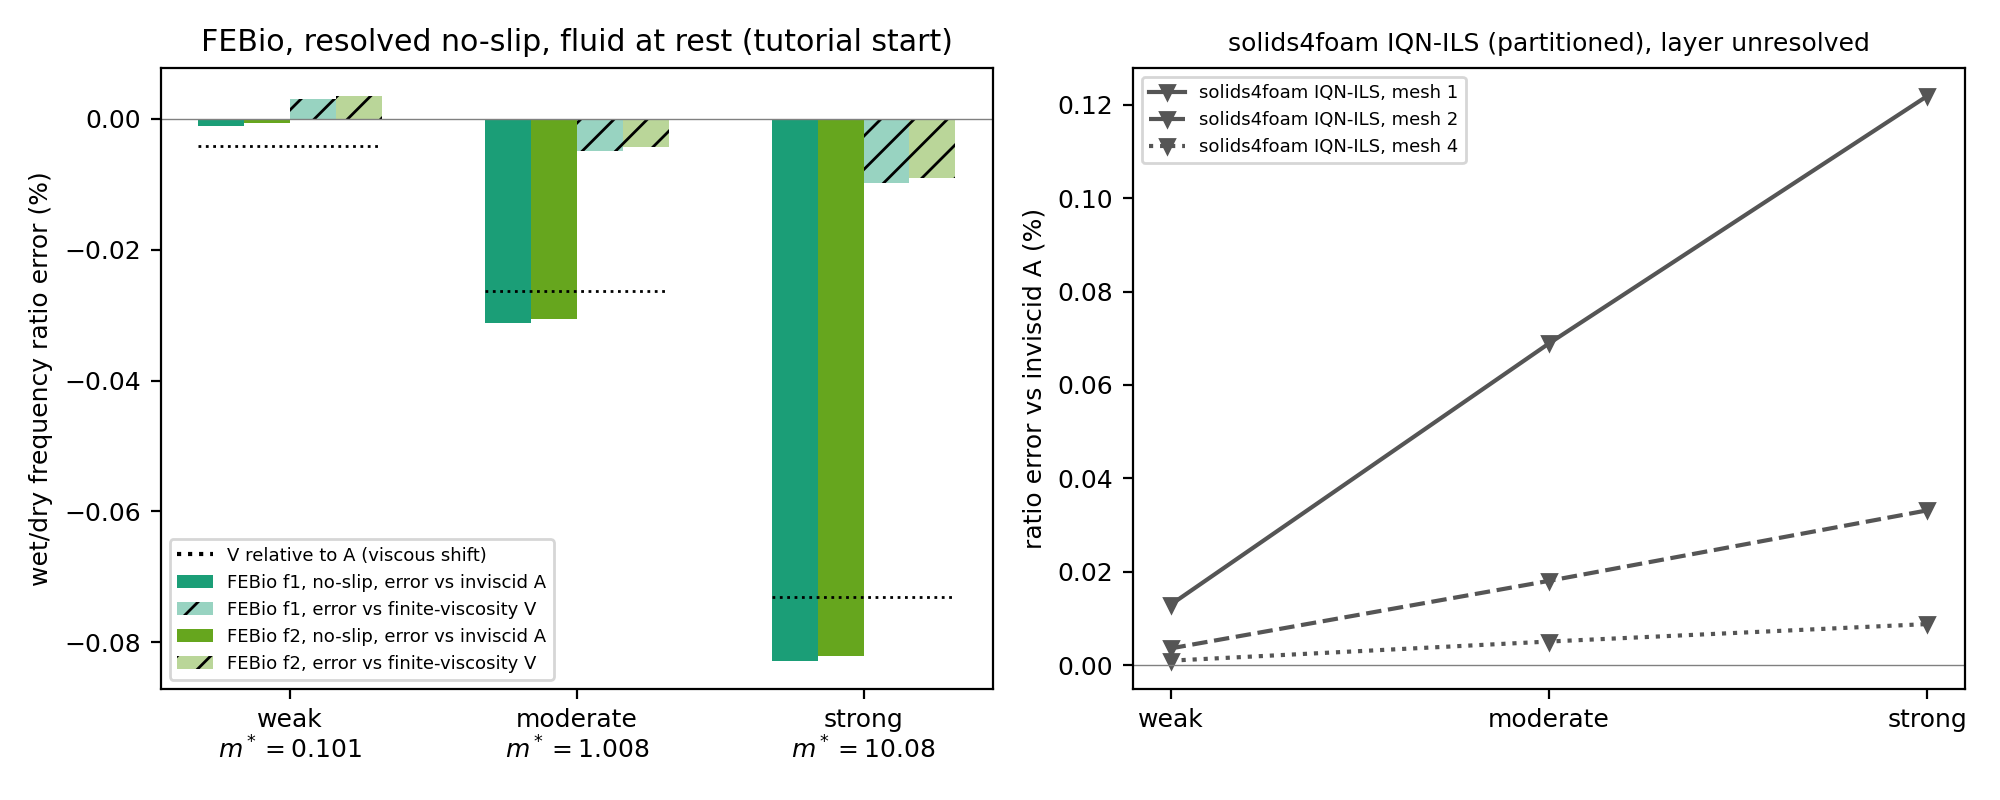
\includegraphics[width=\textwidth]{figures/verification/ringAddedMass_febio_R1}
	\caption{ringAddedMass, wet/dry frequency ratio error. Left: FEBio with resolved no-slip layers and the fluid at rest, against the exact inviscid ratio (A) and the exact finite-viscosity ratio (V), at two ring/tangential resolutions (f1, f2); the dotted lines mark V relative to A. Right: solids4foam (Stokes layer unresolved, standard solid, quasi-monolithic (QM) and IQN-ILS coupling), against A, at mesh factors 1, 2 and 4. The two panels show different discretisations of the same continuum problem; they are not matched meshes. Sources: \texttt{paper-data/febio\_ring\_added\_mass/no\_slip\_resolved/} and \texttt{ringAddedMass\_monolithic\_mesh.csv} (PR~\#13).}
	\label{fig:ring_febio_ratio}
\end{figure}
\begin{figure}[htbp]
	\centering
	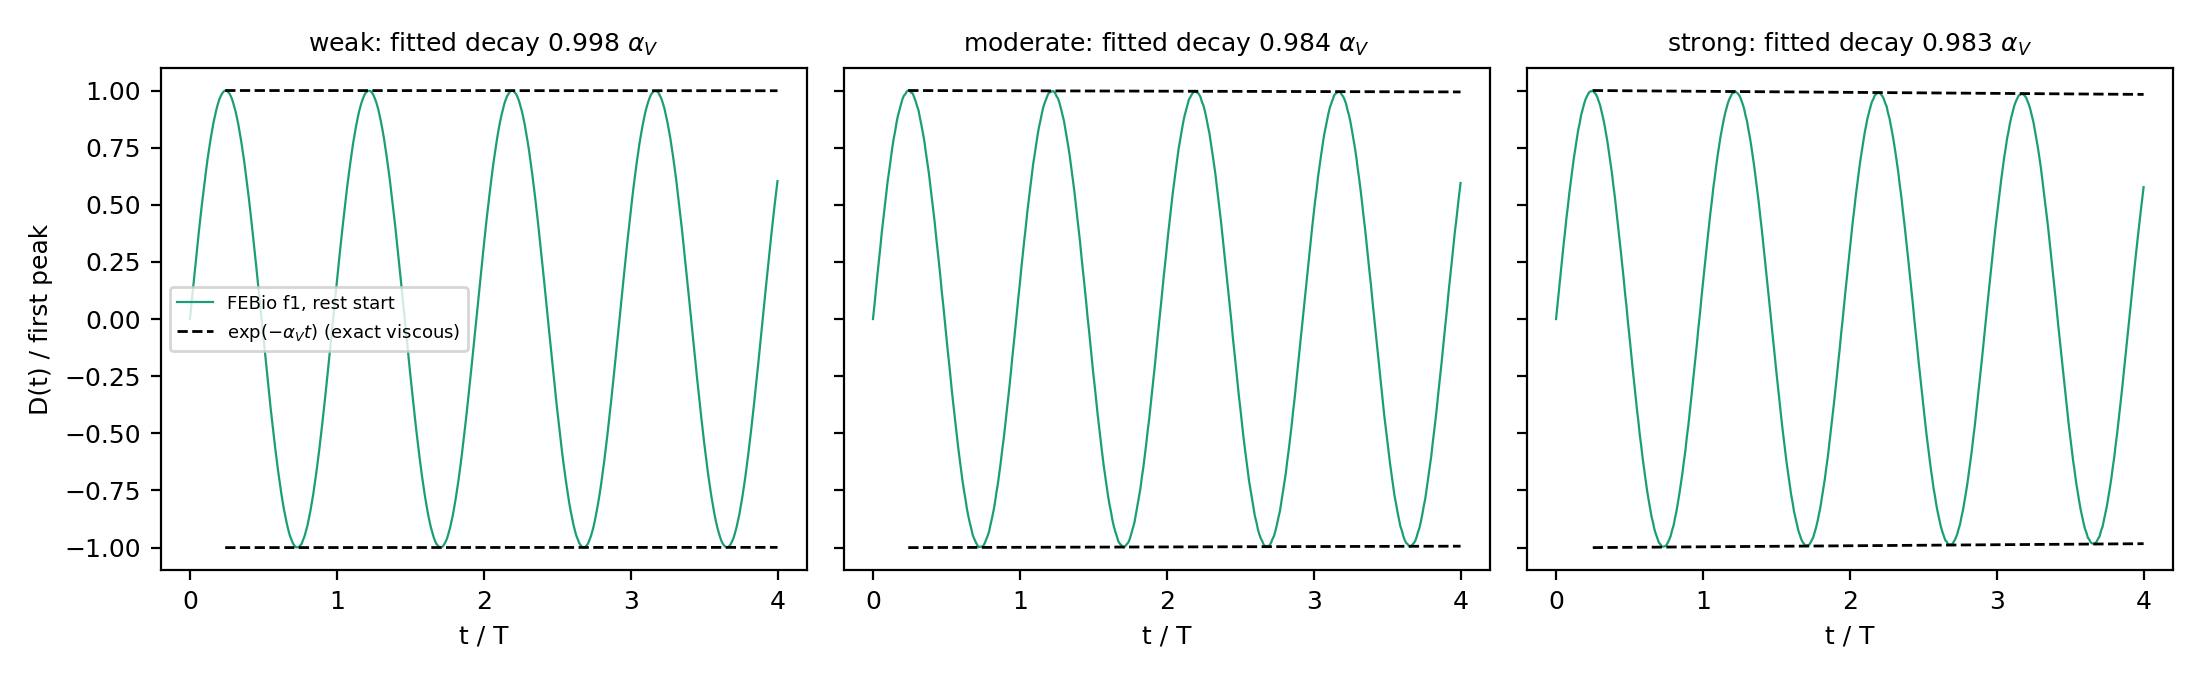
\includegraphics[width=\textwidth]{figures/verification/ringAddedMass_febio_R3}
	\caption{ringAddedMass, FEBio displacement histories $D=(u_r(0^\circ)-u_r(90^\circ))/2$ at the f1 resolution with the fluid at rest, normalised by the first peak, for the weak, moderate and strong levels, with the exact viscous envelope $\exp(-\alpha_V t)$. The fitted decay rates are $0.998$, $0.984$ and $0.983$ times $\alpha_V$.}
	\label{fig:ring_febio_decay}
\end{figure}

\emph{What the solids4foam data do and do not contain.}
Because the tutorial mesh does not resolve the Stokes layer, the solids4foam wet/dry ratio errors against the inviscid reference ($-0.016\%$, $-0.0016\%$, $-0.0001\%$ for the quasi-monolithic coupling at mesh factors 1, 2, 4 in the moderate level) lie on the inviscid side of the reference and cannot discriminate the viscous shift ($-0.026\%$ for that level); its fitted amplitude decay at 100 steps per period ($1.2\times10^{-4}\,\mathrm{s^{-1}}$, moderate, factor 2) is a quarter of the viscous rate and falls by a factor of about 7--9 with each halving of the time step, so it is dominated by temporal damping.
The comparison with FEBio is therefore a comparison of two independent discretisations against the same continuum references at the level of $0.03\%$ in the ratio; the viscous damping and the viscous shift are verified for FEBio only, and a solids4foam verification of these quantities would need a mesh that resolves the layers.

\emph{Interface mechanics.}
The pressure and viscous traction that FEBio's fluid--FSI surface load applies to the ring were reconstructed from logged nodal dilatation and element stress (Figure~\ref{fig:ring_febio_traction}).
The work of the reconstructed traction equals the ring's kinetic plus strain energy change to $0.02$--$0.09\%$ of the energy swing ($1.9\%$ for the strong level started at rest), which checks the orientation, the area measure and the sign independently of the force magnitude, and the $n=2$ viscous shear amplitude is $0.84$--$0.90$ of the thin-Stokes-layer estimate computed from the logged velocities, with a shear-to-pressure traction ratio of $4\times10^{-4}$ to $8\times10^{-4}$.
For the strong level started from the potential-flow field, the energy lost by the fluid including the integrated viscous dissipation balances the work on the ring to $0.5\%$ of the ring's energy swing, and the discrete energy balance is closed to $0.3\%$ of the initial energy.
These are reconstructions and one-element-gradient dissipation estimates, not measured interface forces; the weak level started from the potential-flow field did not converge in its first step and is not reported.
\begin{figure}[htbp]
	\centering
	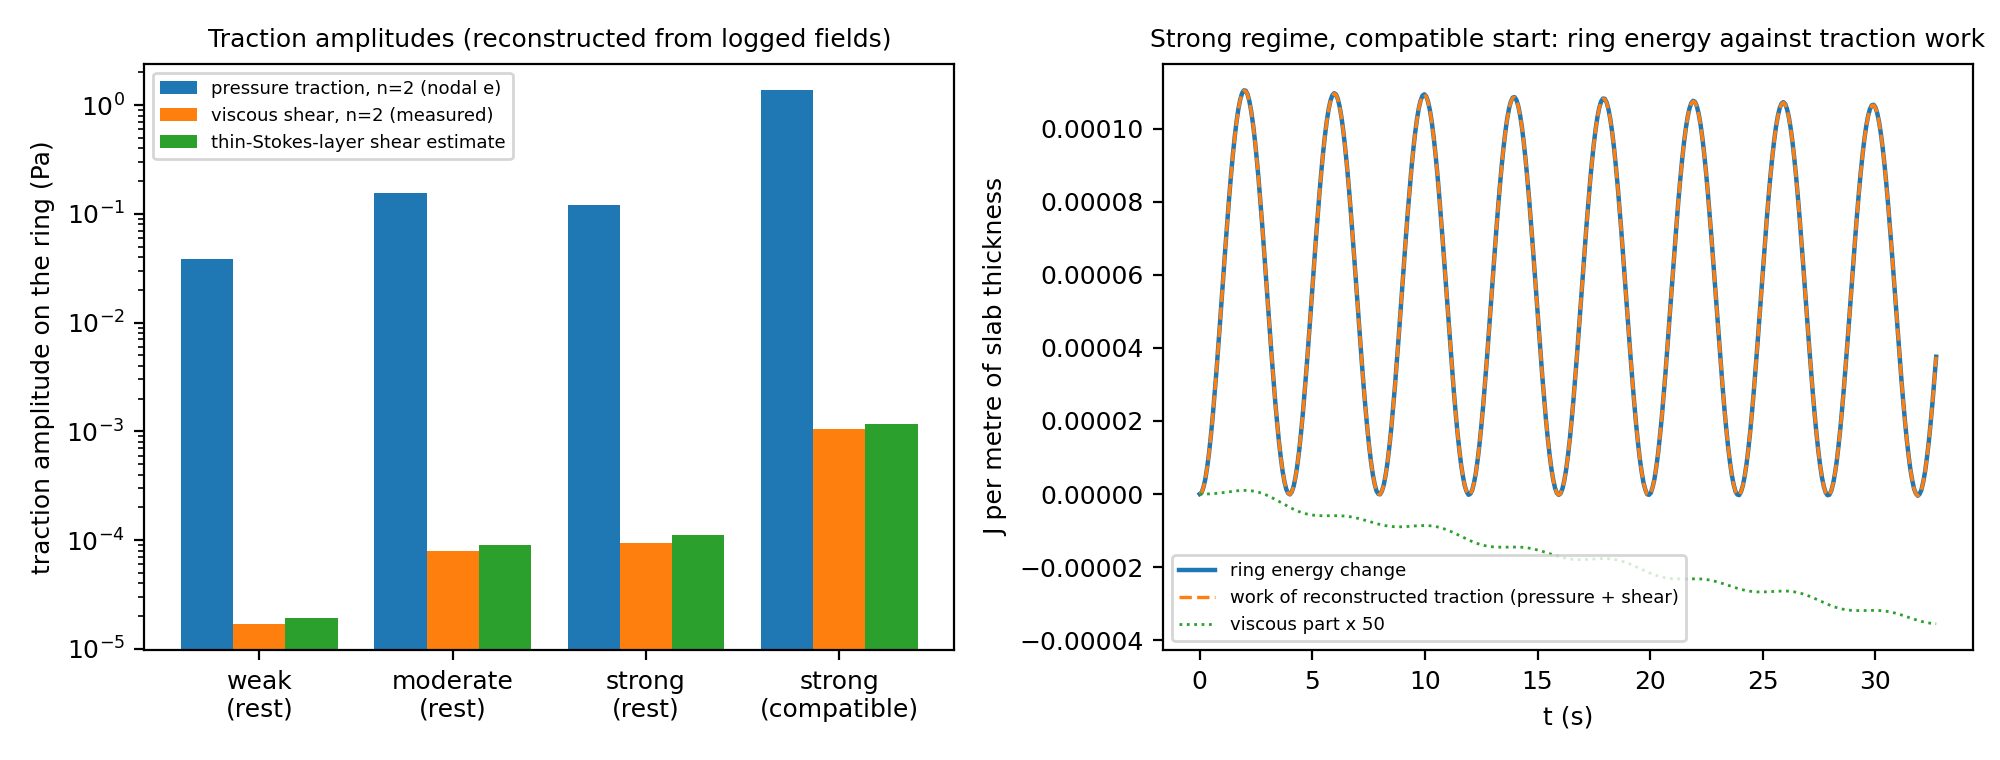
\includegraphics[width=\textwidth]{figures/verification/ringAddedMass_febio_R4}
	\caption{ringAddedMass, FEBio interface traction on the ring, reconstructed from logged fields. Left: $n=2$ amplitudes of the pressure traction, the viscous shear traction and the thin-Stokes-layer shear estimate (fluid at rest, and the strong level from the potential-flow field). Right: strong level, potential-flow start, the ring's energy change and the work of the reconstructed traction (the viscous part, multiplied by 50, is dissipative). Source: \texttt{paper-data/febio\_ring\_added\_mass/no\_slip\_resolved/}.}
	\label{fig:ring_febio_traction}
\end{figure}

\emph{Status.}
FEBio reproduces the finite-viscosity, no-slip ring problem for the three added-mass levels, with the stated model-form differences (weak compressibility, finite strain, finite amplitude, regulariser) quantified at the $0.01$-percentage-point level in the moderate level; it is a qualified independent comparison rather than a demonstration that the two discretisations produce the same discrete solution.
The earlier free-slip FEBio runs of this problem (an analytical-limit study, which agrees with the inviscid ratio to $\leq0.041\%$ at the finest mesh, but with a different wall condition) are kept as a separate record in the evidence package.

\begin{table}[htbp]
	\centering
	\small
	\setlength{\tabcolsep}{4pt}
	\caption{ringAddedMass, FEBio v4.13, no-slip on the ring and the rigid wall, $\nu_F=10^{-7}\,\mathrm{m^2/s}$, fluid initially at rest, fluid mesh graded to a first cell of $\delta/4$ at both walls ($\delta=\sqrt{2\nu_F/\omega}$; 52 radial cells), 100 steps per period, four periods. f1 and f2: ring and tangential resolution ($4\times48$ and $8\times96$ ring cells; $48$ and $96$ tangential fluid cells). Errors of the wet/dry frequency ratio are against the exact inviscid ratio (A) and against the exact finite-viscosity ratio (V, the linearised viscous eigenvalue of the same Chebyshev code, $\mathrm{A}(1+\text{viscous shift})$); the last column is the fitted amplitude decay rate divided by the exact viscous rate $\alpha_V=1.005\times10^{-4}$, $4.748\times10^{-4}$, $5.621\times10^{-4}\,\mathrm{s^{-1}}$. Source: \texttt{paper-data/febio\_ring\_added\_mass/no\_slip\_resolved/}.}
	\label{tab:ring_febio}
	\begin{tabular}{llrrrr}
		\toprule
		Level & Mesh & $\omega$ (rad/s) & Ratio error vs A & Ratio error vs V & Decay$/\alpha_V$ \\
		\midrule
		weak ($m^*=0.101$) & f1 & 2.49852 & $-$0.0010\% & $+0.0031$\% & 0.998 \\
		weak ($m^*=0.101$) & f2 & 2.45089 & $-$0.0006\% & $+0.0035$\% & 0.985 \\
		moderate ($m^*=1.008$) & f1 & 1.85056 & $-$0.0311\% & $-$0.0049\% & 0.984 \\
		moderate ($m^*=1.008$) & f2 & 1.81529 & $-$0.0305\% & $-$0.0043\% & 0.977 \\
		strong ($m^*=10.08$) & f1 & 0.78786 & $-$0.0828\% & $-$0.0097\% & 0.983 \\
		strong ($m^*=10.08$) & f2 & 0.77284 & $-$0.0821\% & $-$0.0090\% & 0.974 \\
		\bottomrule
	\end{tabular}
\end{table}

\paragraph{Lesson.}
The wet/dry ratio isolates the added-mass coupling from solid and temporal errors, which the two runs share, and so verifies it independently of the accuracy of the solid; the exact reference attributes the remaining error to a single source.
Large-amplitude effects are, by design, not tested, and the solids4foam runs do not resolve the viscous layers; viscous damping and the viscous frequency shift are tested only by the independent FEBio comparison above.

%%-------------------------------------------------------------------
\subsubsection{Pulsatile compliant tube}\label{sec:womersley}
%%-------------------------------------------------------------------

\paragraph{What it tests.}
Pressure-wave propagation in a compliant vessel combines added mass, viscous attenuation and wall compliance.
Womersley's analysis~\citep{Womersley1955, Womersley1957} has been used to verify FSI codes~\citep{Filonova2020}, usually in a thin-wall, long-wave form whose modelling error is not negligible for a thick wall.
Here a harmonic wave travels along an untethered axisymmetric tube ($h/R = 0.1$, $L/R = 15$, $\alpha = 5.01$, $\rho_S h/(\rho_F R) = 0.1$), with exact travelling-wave data at both ends (no reflection) and exact initial fields; amplitudes ($\approx5\times10^{-4}R$) are small enough for linear theory to hold to well below $10^{-3}$.

\paragraph{Reference.}
The exact linear solution for a thick linear-elastic cylinder (Chebyshev collocation; 8 and 24 intervals agree to $\approx10^{-11}$) coupled to the full linearised Navier--Stokes equations: $k = 0.143978 - 0.020727\mathrm{i}\,\mathrm{m^{-1}}$, i.e.\ a wave speed of $0.872796\,\mathrm{m/s}$.
It reduces to Womersley's thin-wall equation (Filonova et al., Eq.~41) as $h/R\to0$.
The thin-wall wave speed is $4.7\%$ higher for this wall: used as a reference, it would have hidden every discretisation error studied here.

\paragraph{Evidence.}
First Fourier coefficients over periods 5--6 (period-to-period change $<10^{-4}$) are compared for mesh factors 1, 2, 4 at 200 steps per period and for 50--400 steps per period on the middle mesh (Table~\ref{tab:womersley}), with Robin--Neumann coupling.
The tube ends carry the exact pressure and the exact normal velocity gradient, and the fluid solver makes the mass flux through them consistent with the flux of the boundary velocity to $O(\Delta t\,h)$ (see \emph{Time} below). All values are from the tutorial's verification driver (\texttt{Allverify}) with this configuration.

\begin{table}[htbp]
	\centering
	\small
	\setlength{\tabcolsep}{4pt}
	\caption{womersleyTube: observed orders from successive differences (three levels) and finest-mesh errors against the exact solution (mesh factor 4, 200 steps per period). Time orders on mesh factor 2 from 50/100/200 and 100/200/400 steps per period. The profile mesh order is from its errors on the two finest meshes. Phases in radians. Flux-consistent tube ends (\texttt{fluxConsistentPatches}); solids4foam commit a507bfd41, OpenFOAM-v2512, Linux (x86\_64), \texttt{Allverify}.}
	\label{tab:womersley}
	\begin{tabular}{lrrr}
		\toprule
		Quantity & Mesh order & Time order & Finest-mesh error \\
		\midrule
		velocity profile (max.) & 2.04 & -- & $1.20\times10^{-3}$ \\
		flow-rate amplitude & 2.05 & 2.04, 2.05 & $-3.09\times10^{-4}$ \\
		flow-rate phase & 1.92 & 1.86, 1.91 & $8.2\times10^{-5}$ \\
		wall displacement amplitude & 2.01 & 1.96, 1.97 & $-1.76\times10^{-4}$ \\
		wall displacement phase & 1.40 & 2.14, 2.06 & $-1.15\times10^{-3}$ \\
		wave speed & 2.02 & 1.94, 1.97 & $1.4\times10^{-5}$ \\
		attenuation, $\mathrm{Im}(k)$ & -- & 2.10, 2.07 & $-1.96\times10^{-3}$ \\
		\bottomrule
	\end{tabular}
\end{table}

\begin{itemize}
	\item \emph{Space.} The profile, flow rate, wall-displacement amplitude and wave speed converge at second order (2.01--2.05; flow phase 1.92), the wave speed to $1.4\times10^{-5}$ on the finest mesh. The wall-displacement phase converges more slowly (order 1.40). The attenuation error is $\approx-2\times10^{-3}$ on all three meshes and at every time step: it no longer depends on the discretisation, and is consistent with the linear-theory level ($\approx10^{-3}$) amplified about sevenfold, since $\mathrm{Im}(k)$ is only $14\%$ of $\mathrm{Re}(k)$.
	\item \emph{Time.} Over the steps used, every QoI converges at second order (1.91--2.07 from 100/200/400 steps per period, 1.86--2.14 from 50/100/200), in both the 5--6 and the 11--12 period windows. With the end condition imposed as usual (a mixed velocity condition with zero value fraction and a fixed pressure), the same study gave 1.29--1.84 from 50/100/200 and 0.75--1.79 from 100/200/400 steps per period, falling towards first order, on every mesh. The cause was an $O(\Delta t)$ inconsistency of the end flux: the segregated pressure--velocity algorithm treats a mixed velocity condition as fixing the boundary velocity, so the end flux is $\mathbf{U}_b\cdot\mathbf{S}_f - (\Delta t/\gamma)\,\partial p/\partial n\,|\mathbf{S}_f|$ (with $\gamma$ the BDF2 leading coefficient), which differs from the boundary velocity flux by a term proportional to $\Delta t$ and to the axial pressure gradient, about 1--2\% of the end flux at the working steps. The behaviour was identical for IQN-ILS and Robin--Neumann, persisted in a fluid-only computation with the exact wall motion on a static mesh, and was independent of the mesh, the start-up, the analysis window, the Rhie--Chow \texttt{ddtCorr} term and the tolerances (tightened 100-fold). Giving the pressure-equation flux on the end patches the boundary velocity (and the pressure gradient of the boundary cell, so that the fixed pressure stays implicit) removes it, with the boundary data unchanged; the time error at 200 steps per period falls from $1.6$, $0.9$ and $3.8\times10^{-3}$ to $1.3\times10^{-4}$, $3.3\times10^{-5}$ and $1.6\times10^{-4}$ in the wall amplitude, wave speed and attenuation. The treatment is not exact: the boundary-cell pressure gradient differs from the fixed-value normal gradient used by the pressure equation by $-(h/4)\,\partial^2 p/\partial n^2$ (measured with the solver's operators on the exact pressure on all three meshes), so an end-flux inconsistency of $O(\Delta t\,h)$ remains, the same as for a standard fixed-pressure outlet. At fixed mesh the scheme is therefore formally first order in time as $\Delta t\to0$, with a coefficient that vanishes with $h$, and second order under joint refinement of $h$ and $\Delta t$. In a fluid-only computation on the coarsest mesh the observed order turns towards one only beyond $\approx3200$ steps per period (1.97, then 1.57), and by the $h$-scaling beyond $\approx6400$ on the study mesh, against at most 400 used here; a variant that imposes the end flux exactly stays at second order (2.00--2.08) but over-determines the pressure equation (fixed pressure and prescribed flux on the same boundary) and did not converge robustly. (At such fine fixed-mesh time steps, the default flux-ratio coefficient of OpenFOAM's Rhie--Chow \texttt{ddtCorr} term also limits convergence, at $\approx10^{-6}$.)
	\item \emph{Start-up.} The tutorial initialisation originally set the old-time solid displacements to the exact solution in the cells but left their boundary values at zero; through the Robin condition, which imposes the solid's boundary acceleration on the fluid, this produced a first-period transient that grew as $\Delta t$ was reduced ($3.4\%$ of the amplitude at 400 steps per period). The tutorial now sets exact boundary values, and the transient is $0.2$--$0.3\%$ from 100 to 400 steps per period. Either way it does not reach the analysed periods 5--6 (effect $<3\times10^{-6}$; period-to-period change $\leq7\times10^{-5}$). It also explains a $0.26\%$ shift of a Robin--Neumann regression value between OpenFOAM-v2412 and v2512, which was confined to the start-up: with exact boundary values the two versions agree to $10^{-8}\,\mathrm{m}$ ($3\times10^{-5}$ of the amplitude).
	\item \emph{Space--time balance.} At 200 steps per period the remaining time error is a tenth or less of the finest-mesh error for the profile, wall phase and attenuation, comparable for the wall amplitude and flow phase, and larger for the wave speed, whose finest-mesh error is only $1.4\times10^{-5}$.
	\item \emph{Coupling.} IQN-ILS and Robin--Neumann agree to $2.2\times10^{-4}$ or better in every QoI (14.6 against 9.3 coupling iterations per step).
\end{itemize}

\todo{The numbers in Table~\ref{tab:womersley} use the \texttt{pimpleFluid} option \texttt{fluxConsistentPatches} on the tube ends (solids4foam PR \#533, branch \texttt{womersley-temporal-investigation}, commit a507bfd41; OpenFOAM-v2512, Linux), where the option and the exact old-time boundary values are set in the tutorial and the table is the output of the full \texttt{Allverify} on that commit. Not yet merged: confirm the commit hash after merging. Investigation, data and the original-set-up results: \texttt{womersleyTube/verification/womersley\_temporal\_investigation.md} (formal order of the end treatment: Section 15 there).}

\paragraph{Lesson.}
This viscous wave-propagation case complements ringAddedMass (inviscid, standing mode) with separate amplitude and phase QoIs.
Its temporal study first showed orders below the nominal two, falling towards one with refinement; the exact reference, together with fluid-only and end-flux diagnostics, traced this to an $O(\Delta t)$ mass-flux inconsistency in the boundary treatment of the truncated domain rather than to the fluid--solid coupling, and a flux-consistent end treatment restores second order in every QoI over the steps used; formally, a boundary term of $O(\Delta t\,h)$ remains, so at fixed mesh the order would tend to one at much smaller steps.
A truncated-domain benchmark therefore verifies its boundary treatment as much as its interior scheme, and a sub-nominal temporal order should be traced before it is attributed to the coupling.
Limitations: the wall is untethered, unlike Womersley's constrained tube (solids4foam issue \#511), the high-order solid cannot be used on wedge meshes (issue \#512), and the attenuation is limited to $\approx0.2\%$ by the linear theory.


%%%%%%%%%%%%%%%%%%%%%%%%%%%%%%%%%%%%%%%%%%%%%%%%%%%%%%%%%%%%%%%%%%
\subsection{Independently converged numerical reference}\label{sec:independent_refs}
%%%%%%%%%%%%%%%%%%%%%%%%%%%%%%%%%%%%%%%%%%%%%%%%%%%%%%%%%%%%%%%%%%

%%-------------------------------------------------------------------
\subsubsection{Collapsible channel}\label{sec:collapsible}
%%-------------------------------------------------------------------

\paragraph{What it tests.}
A thin, very light elastic wall in a channel combines strong added mass, bending-dominated large deformation and fluid-mesh motion, where partitioned methods are least robust~\citep{Jensen2003, Heil2004, Heil2008}.
An elastic section of the upper wall ($h/L = 0.005$; St Venant--Kirchhoff continuum) collapses under a ramped external pressure to $\approx21\%$ of the channel width and then performs a damped oscillation ($Re = Re\,St = 50$; analysed to $t = 1.5\,\mathrm{s}$).
The problem \emph{modifies} that of Jensen and Heil (no pre-stress, $h/a = 1/20$, clamped ends, pressure ramp, regularising density $\rho_S = \rho_F$, which shifts the response by $0.28\%$ of the peak) so that it is well posed for a continuum solid and partitioned coupling; the published values are therefore not reproduced.

\paragraph{Reference and model-form difference.}
The reference (category B) is computed with oomph-lib~\citep{Heil2006}, an independent monolithic Newton finite element code whose driver source is stored with the case.
It is Richardson-extrapolated in time, with an uncertainty of $\approx0.3\%$ of the peak displacement dominated by its spatial error (levels 1 and 2 differ by $0.26\%$; Richardson correction $0.06\%$; two fluid element types differ by $<0.001\%$).
oomph-lib represents the wall as a geometrically nonlinear Kirchhoff--Love \emph{beam}, whereas the code under test resolves it as a two-dimensional continuum.
This model-form difference is explicitly identified, is of order $h/L$, and is quantified as $0.05\%$ for the static deflection; it is small relative to the numerical errors of interest, which is why the reference is treated as category B.
A difference below the reference uncertainty plus this contribution cannot be attributed to either code.

\paragraph{Evidence.}
The QoI is the wall-midpoint vertical displacement history, with the first trough as scalar summary.

\begin{figure}[htbp]
	\centering
	% Source: solids4foam development, tutorials/fluidSolidInteraction/collapsibleChannel/verification/reference/mesh_study_wallMid.png (PR #507).
	\includegraphics[width=0.85\textwidth]{figures/verification/collapsibleChannel_mesh_study_wallMid}
	\caption{collapsibleChannel: wall-midpoint vertical displacement for fluid-mesh levels F1--F4 (solid mesh $160\times8$, $\Delta t = 0.00625\,\mathrm{s}$, high-order solid, Robin--Neumann coupling) against the oomph-lib reference. Interim figure reproduced from the solids4foam verification output.}
	\label{fig:collapsible_mesh}
\end{figure}
\todo{Replace Figure~\ref{fig:collapsible_mesh} with a publication-quality version (legend labels, inset at first trough and second peak, error-versus-$h$ panel). The current PNG legend shows raw run identifiers.}

\begin{itemize}
	\item \emph{Solid.} In a static wall test the cubic high-order solid is within $0.25\%$ of oomph-lib on all solid meshes and converges to the $0.05\%$ model-form difference; the linear-reconstruction solid has errors from $-16.7\%$ to $-0.22\%$. In the coupled problem on the tutorial mesh the solid contributes $0.44\%$ (cubic) against $17.4\%$ (linear).
	\item \emph{Fluid mesh.} Four levels (3\,200 to 51\,200 cells, fixed $\Delta t = 0.00625\,\mathrm{s}$, compared with oomph-lib at the same $\Delta t$): the error falls from $4.65\%$ to $1.43\%$, $0.53\%$ and $0.50\%$ of the peak (orders 1.7 and 2.4, then a floor; Fig.~\ref{fig:collapsible_mesh}). The floor is of the size of the reference uncertainty plus the model-form contribution; the finest first trough is $-0.21610\,\mathrm{m}$ against $-0.2160\,\mathrm{m}$ for the converged reference.
	\item \emph{Time.} On the coarsest fluid mesh, successive differences of $4.56\%$, $1.33\%$ and $0.34\%$ give orders 1.8 and 2.0 (oomph-lib itself: 1.8 and 1.9).
	\item \emph{Coupling.} IQN-ILS and Robin--Neumann agree to $0.08$--$0.23\%$ of the peak, but this gap does \emph{not} decrease with mesh refinement and is of the size expected from the coupling tolerance. In a wall-density sweep ($\rho_S/\rho_F = 0$--3) IQN-ILS fails to complete for part of the range, whereas Robin--Neumann completes for all $\rho_S/\rho_F \geq 1$.
\end{itemize}

\paragraph{Lesson.}
This is the strongest independent-code comparison in the suite.
For a thin bending-dominated wall the solid discretisation can dominate the FSI error, and once the discretisation error falls to $\approx0.5\%$ the reference uncertainty, model-form difference and coupling tolerance are of comparable size, so closer agreement requires tightening all three.
Limitations: the temporal error on the finer fluid meshes is not measured; the high-order solid is serial only, and a 4-rank linear-reconstruction run gave an incorrect displacement that remains to be re-checked.


%%%%%%%%%%%%%%%%%%%%%%%%%%%%%%%%%%%%%%%%%%%%%%%%%%%%%%%%%%%%%%%%%%
\subsection{Classical FSI benchmarks revisited}\label{sec:classical}
%%%%%%%%%%%%%%%%%%%%%%%%%%%%%%%%%%%%%%%%%%%%%%%%%%%%%%%%%%%%%%%%%%

These benchmarks are widely used, but their published values carry incompletely quantified error, are inconsistent between sources, or both.
The present calculations are first assessed by self-convergence, and the comparison with the literature is then used to examine the published values themselves.

%%-------------------------------------------------------------------
\subsubsection{Hron--Turek family (FSI1, FSI2, FSI3)}\label{sec:fsi1}\label{sec:fsi23}
%%-------------------------------------------------------------------

\begin{figure}[htbp]
	\centering
	\includegraphics[scale=1]{figures/HronTurek3-geometry}
	\caption{Hron--Turek benchmark geometry (shown for FSI3; FSI1 and FSI2 share the geometry).}
	\label{fig:hronturek_geom}
\end{figure}

\paragraph{What it tests.}
An elastic flag attached to a rigid cylinder in a channel~\citep{Turek2006} (Fig.~\ref{fig:hronturek_geom}).
FSI1 ($Re = 20$) is steady, with small but geometrically nonlinear deformation; FSI3 ($Re = 200$, $\rho_S = \rho_F$) is a self-excited, high-frequency oscillation at low mass ratio ($u_y \approx \pm35\,\mathrm{mm}$); FSI2 ($Re = 100$, heavier and softer flag) is a large-amplitude flapping ($u_y \approx \pm80\,\mathrm{mm}$) that strongly distorts the fluid mesh.

\paragraph{Reference.}
For FSI1 the Featflow results are tabulated on six levels (finest $\approx10^6$ elements), with a spread across levels of $0.73\%$ ($u_x$), $0.19\%$ ($u_y$), $0.14\%$ (drag) and $0.26\%$ (lift); the finest values ($u_x = 2.2705\times10^{-5}\,\mathrm{m}$, $u_y = 8.2088\times10^{-4}\,\mathrm{m}$, drag $14.2943\,\mathrm{N/m}$, lift $0.76375\,\mathrm{N/m}$) are category B.
For FSI2 and FSI3 the references are the Featflow level-4 tables (FSI3: 15\,872 elements, $\Delta t = 0.00025\,\mathrm{s}$), and both are category C.
Their own uncertainty is not small: between Featflow levels 3 and 4 the FSI2 values change by $0.9$--$2.5\%$, and the FSI3 values by $3.8\%$ ($u_x$ mean), $4.0\%$ ($u_x$ amplitude), $4.5\%$ (drag amplitude), $2.6\%$ (lift amplitude) and $1.6\%$ ($u_y$ amplitude), non-monotonically except for the drag mean and the lift amplitude, which rises by $\approx4\,\mathrm{N/m}$ per level.
The FSI3 reference is therefore uncertain by $\approx3$--$5\%$ in $u_x$ and the force amplitudes and $\approx2\%$ in the $u_y$ amplitude; only the drag mean ($0.3\%$) and the frequency are known to $\lesssim0.3\%$.
The Featflow tables are among the most carefully documented FSI references available, and the Hron--Turek problems owe much of their influence to the multi-level results published with them; the points below concern how far those results can bound the error of another code, not their value as a benchmark.
For the FSI3 displacements and drag amplitude, the Featflow levels 2, 3 and 4 do not form a monotone sequence ($u_y$ amplitude $35.73$, $34.43$, $34.99\,\mathrm{mm}$; $u_x$ mean $-3.02$, $-2.77$, $-2.88\,\mathrm{mm}$; drag amplitude $28.80$, $26.50$, $27.74\,\mathrm{N/m}$), and the lift amplitude rises by $\approx4\,\mathrm{N/m}$ per level without settling. These quantities have therefore not been shown to be in the asymptotic range, and no extrapolated value or error bound can be formed from them.
The published reference time history is not strictly periodic either: over its $7.9$ periods the per-period lift amplitude drifts from $157.7$ to $153.5\,\mathrm{N/m}$ ($2.7\%$), so the tabulated amplitudes also depend on the averaging window by about that amount.
Together these bound the confidence that can be placed in the level-4 values to a few percent for the displacements and force amplitudes, whereas the frequency and the drag mean, which change little between levels, are well determined.
The detailed Featflow tables, used here, differ from the frequently quoted summary values of~\citet{Turek2006} (Table~\ref{tab:hronturek_ref}), most strongly in the FSI3 drag amplitude ($-18\%$), and the summary frequencies are rounded; the summary values are level 4 of the 2006 proceedings table at $\Delta t = 0.0005\,\mathrm{s}$, which the Featflow pages retain only as superseded values. A comparison with the summary values would misattribute this $18\%$ to the code under test.
As a check, the driver reproduces the tabulated statistics from the published Featflow time histories to within $0.6\%$ (FSI3; $0.8\%$ for drag amplitude, $0.3\%$ for the frequencies) and $0.3\%$ (FSI2).
\todo{Cite the Featflow table source precisely (Turek--Hron benchmark web pages / Turek et al.\ 2010 book chapter?)~\citetodo{Featflow FSI benchmark tables}; confirm the FSI1 six-level spread from that source. Check every entry of Table~\ref{tab:hronturek_ref} against the original sources rather than the solids4foam README; identify which later papers quote which set.}

\begin{table}[htbp]
	\centering
	\small
	\setlength{\tabcolsep}{5pt}
	\caption{Hron--Turek FSI3 and FSI2: frequently quoted summary values of~\citet{Turek2006} against the Featflow level-4 tables used here (amplitudes; frequencies in brackets). Units: mm for displacements, N/m for forces. Source: solids4foam \texttt{HronTurek/verification/README.md} and reference JSON.}
	\label{tab:hronturek_ref}
	\begin{tabular}{llll}
		\toprule
		Case & Quantity & Summary~\citep{Turek2006} & Featflow table \\
		\midrule
		FSI3 & $u_y$ amplitude & 34.38 [5.3\,Hz] & 34.99 [5.46\,Hz] \\
		FSI3 & drag amplitude & 22.66 & 27.74 \\
		FSI3 & lift amplitude & 149.78 & 153.91 \\
		FSI2 & $u_y$ amplitude & 80.6 [2.0\,Hz] & 81.6 [1.93\,Hz] \\
		FSI2 & drag amplitude & 73.75 & 77.65 \\
		FSI2 & lift amplitude & 234.2 & 237.8 \\
		\bottomrule
	\end{tabular}
\end{table}

\paragraph{Evidence.}
FSI3 has three mesh levels (1x: 5\,336 fluid and 630 solid cells; 2x: 21\,344 and 2\,520; 4x: 85\,376 and 10\,080; ratio 2 in the plane), with $\Delta t = 0.001$, $0.0005$ and $0.00025\,\mathrm{s}$ (IQN-ILS, coupling tolerance $10^{-5}$, OpenFOAM-v2512); every coupled step of every level met the interface tolerance (mean 7.0, 7.0 and 6.7 iterations per step).
FSI1 and FSI2 have two levels (1x and 2x). FSI1 is integrated in pseudo-time; for FSI2/FSI3, $\Delta t$ is halved with the mesh.
Statistics are taken over the last full $u_y$ period of the closing second of a 7\,s run.
This sequence uses the tutorial set-up (velocity-based Laplacian mesh motion, zero-gradient pressure on the flag). The diagnosis below led to a corrected set-up, whose sequence is given in Table~\ref{tab:hronturek_corrected}.

\begin{table}[htbp]
	\centering
	\small
	\setlength{\tabcolsep}{4pt}
	\caption{Hron--Turek FSI3, tutorial set-up: three-level results ($\Delta t$ halved with $h$; IQN-ILS), error of the 4x value against the Featflow level-4 table, and observed order from successive differences. Force amplitudes are 4\,ms moving averages, which remove the coupling noise of the finest time step (see text). Units: mm, Hz, N/m. Source: paper-data/hronturek\_fsi3\_4x\_findings.md, Section~4.}
	\label{tab:hronturek}
	\begin{tabular}{lrrrrrr}
		\toprule
		Quantity & 1x & 2x & 4x & Featflow & Error 4x & Order \\
		\midrule
		$u_x$ mean & $-2.232$ & $-2.788$ & $-3.085$ & $-2.880$ & $-7.1\%$ & 0.91 \\
		$u_x$ amplitude & 2.163 & 2.657 & 2.917 & 2.720 & $+7.2\%$ & 0.93 \\
		$u_y$ amplitude & 29.85 & 34.18 & 36.23 & 34.99 & $+3.5\%$ & 1.07 \\
		$u_y$ frequency & 5.588 & 5.523 & 5.474 & 5.460 & $+0.25\%$ & --$^a$ \\
		drag mean & 456.6 & 459.7 & 462.1 & 460.5 & $+0.3\%$ & --$^b$ \\
		drag amplitude & 22.63 & 27.63 & 30.63 & 27.74 & $+10.4\%$ & 0.74 \\
		lift amplitude & 228.8 & 172.3 & 165.6 & 153.9 & $+7.6\%$ & --$^c$ \\
		\bottomrule
		\multicolumn{7}{l}{\footnotesize $^a$ Time-step and coupling effects ($\leq0.4\%$) as large as the 2x$\to$4x change. $^b$ 2x$\to$4x change within the late-time} \\
		\multicolumn{7}{l}{\footnotesize variability. $^c$ Ratio 0.12, apparent order 3.1, above the formal order: pre-asymptotic.}
	\end{tabular}
\end{table}

\begin{table}[htbp]
	\centering
	\small
	\setlength{\tabcolsep}{3pt}
	\caption{Hron--Turek FSI3, corrected set-up: fluid meshes refined additionally around the cylinder and over the flag and wake (1x$'$: 11\,764, 2x$'$: 47\,056, 4x$'$: 188\,224, 8x$'$: 752\,896 cells), solid 2x/4x/8x/16x, central convection, acceleration-consistent wall pressure, displacement-based mesh motion, strict coupling test (tolerance $10^{-5}$); $\Delta t = 0.0005\,\mathrm{s}$ on 1x$'$--4x$'$ and $0.00025\,\mathrm{s}$ on 8x$'$ (unstable at $0.0005\,\mathrm{s}$; text); five periods before $t = 6\,\mathrm{s}$, benchmark definitions. $D_2$: 4x$'\to$8x$'$ change; time and coupling: change from halving $\Delta t$ from $0.0005$ to $0.00025\,\mathrm{s}$ on 2x$'$ and from the coupling tolerance ($10^{-4}$ against $10^{-5}$, 1x$'$), relative to $D_2$. Units: mm, Hz, N/m. Source: paper-data/hronturek\_fsi3\_4x\_findings.md, Sections~20 and~21.}
	\label{tab:hronturek_corrected}
	\begin{tabular}{lrrrrrrr}
		\toprule
		Quantity & 1x$'$ & 2x$'$ & 4x$'$ & 8x$'$ & Featflow & 8x$'$ vs Featflow & Time, coupling vs $D_2$ \\
		\midrule
		$u_x$ (max+min)/2 & $-2.859$ & $-3.082$ & $-3.069$ & $-3.010$ & $-2.880$ & $+4.5\%$ & 0.05, 0.05 \\
		$u_x$ amplitude & 2.754 & 2.929 & 2.903 & 2.842 & 2.720 & $+4.5\%$ & 0.04, 0.04 \\
		$u_y$ amplitude & 34.62 & 36.17 & 36.12 & 35.77 & 34.99 & $+2.2\%$ & 0.03, 0.06 \\
		frequency & 5.570 & 5.497 & 5.473 & 5.465 & 5.460 & $+0.1\%$ & 0.07, 0.06 \\
		drag (max+min)/2 & 458.5 & 461.4 & 461.5 & 461.2 & 460.5 & $+0.1\%$ & 0.12, 0.23 \\
		lift amplitude & 194.7 & 174.1 & 164.7 & 159.3 & 153.9 & $+3.5\%$ & 0.00, 0.03 \\
		\bottomrule
		\multicolumn{8}{l}{\footnotesize The force amplitudes depend strongly on the solid mesh (text).}
	\end{tabular}
\end{table}

\begin{table}[htbp]
	\centering
	\small
	\setlength{\tabcolsep}{5pt}
	\caption{Hron--Turek FSI2: relative errors against the Featflow level-4 table on the 1x and 2x meshes (IQN-ILS). The 1x errors were computed from the tabulated values in the evidence inventory.}
	\label{tab:hronturek_fsi2}
	\begin{tabular}{lrr}
		\toprule
		Quantity & 1x & 2x \\
		\midrule
		$u_x$ mean & $21.6\%$ & $3.1\%$ \\
		$u_x$ amplitude & $16.4\%$ & $1.9\%$ \\
		$u_y$ amplitude & $12.4\%$ & $1.3\%$ \\
		$u_y$ frequency & $6.9\%$ & $1.8\%$ \\
		drag mean & $4.6\%$ & $0.5\%$ \\
		drag amplitude & $13.1\%$ & $2.0\%$ \\
		lift amplitude & $7.9\%$ & $7.8\%$ \\
		\bottomrule
	\end{tabular}
\end{table}

\begin{itemize}
	\item \emph{FSI1.} On the 2x mesh the errors against the Featflow finest level are $0.97\%$ ($u_x$), $4.64\%$ ($u_y$), $0.24\%$ (drag) and $1.55\%$ (lift), with two-level apparent orders of 1.5--1.7. The pseudo-time step changes $u_y$ and drag by $0.04\%$ and $u_x$ by $0.26\%$; IQN-ILS and Robin--Neumann agree to $0.01\%$; a fluid-solver tolerance change from $10^{-6}$ to $10^{-9}$ alters the steady values by at most $2\times10^{-4}$. The transverse tip displacement is the slowest-converging QoI.
	\item \emph{FSI3 displacements.} The displacements converge monotonically at an observed order of $\approx0.9$--$1.1$, half the nominal order (Table~\ref{tab:hronturek}): the $u_x$ mean is $-2.232$, $-2.788$ and $-3.085\,\mathrm{mm}$ and the $u_y$ amplitude $29.85$, $34.18$ and $36.23\,\mathrm{mm}$. The 2x--4x changes ($6.0\%$ in $u_y$, $\approx10\%$ in $u_x$) are about ten times the late-time variability of the statistics, so they are resolved. The apparent agreement of the 2x mesh with Featflow ($2$--$3\%$) was a crossing: at 4x the displacements lie beyond the Featflow values ($u_y$ amplitude $+3.5\%$, $u_x$ mean $-7.1\%$) and are still moving away. The two-level apparent orders of 2.6--3.8 reported earlier for this case were artefacts of that crossing and are withdrawn. The $u_x$ mean is not an independent QoI: its time mean is kinematically tied to the transverse motion and scales as $A^{1.88\text{--}1.93}$ with the $u_y$ amplitude $A$ across the levels ($A^2$ to within $1.6\%$ at 1x and $0.4\%$ at 4x), so its sequence follows that of $u_y$. These are the tutorial-set-up values; the diagnosis below traces the first-order behaviour to the set-up, and the corrected sequence (Table~\ref{tab:hronturek_corrected}) no longer shows it.
	\item \emph{FSI3 frequency and drag mean.} The frequency converges onto Featflow ($+0.25\%$ at 4x) and the drag mean lies within $0.3\%$ of it; both are within the reference uncertainty, and the time-step and coupling contributions to the frequency are as large as its 2x--4x change.
	\item \emph{FSI3 force amplitudes.} At the 4x time step the coupling tolerance of $10^{-5}$ leaves step-to-step force noise (lift $7.3\,\mathrm{N/m}$ rms), which inflates the extrema-based amplitudes to $+15.0\%$ (lift) and $+18.1\%$ (drag) above Featflow; tightening the tolerance to $10^{-6}$ reduces the noise eightfold. With the noise filtered, the lift amplitude falls from $11.9\%$ to $7.6\%$ above Featflow with a strongly decelerating sequence (ratio 0.12), and the drag amplitude is still rising. Neither is shown to be asymptotic.
	\item \emph{FSI3 time step and coupling.} On the 2x mesh, halving $\Delta t$ and tightening the coupling tolerance from $10^{-5}$ to $10^{-6}$ change the displacements by at most $1.7\%$, a small fraction of the 2x--4x change, so the scaled path is dominated by the mesh. At $\Delta t = 0.00025\,\mathrm{s}$ IQN-ILS did not reach a tolerance of $10^{-6}$ (it stalled at $5$--$9\times10^{-6}$), so the 4x iterative error is bounded from the 2x pair at that step.
	\item \emph{Lift amplitude (FSI2).} The error is $7.9\%$ and $7.8\%$, i.e.\ not converging over this range, of which $\approx2.4$ percentage points are attributed to coupling-iteration noise.
	\item \emph{Coupling tolerance (FSI2).} With a coupling tolerance of $10^{-5}$ the lift amplitude is inflated by $13\%$ (1x) and $30\%$ (2x) relative to $10^{-6}$ and $10^{-7}$, which agree. A tolerance adequate for displacements is therefore not adequate for the lift, and the inadequacy grows with mesh refinement.
	\item \emph{Coupling algorithm (FSI3).} Robin--Neumann and IQN-ILS histories differ ($u_x$ $5.1\%$ and $1.9\%$, lift $3.5\%$ and $2.8\%$ on 1x and 2x), but the difference decreases with refinement and is smaller than the 1x$\to$2x change; it is attributed to the different discrete interface condition of the Robin--Neumann scheme, not to iterative error.
	\item \emph{Mesh motion (FSI2).} Fluid-mesh non-orthogonality reaches $58^\circ$ by $t = 10.5\,\mathrm{s}$, where the analysis window is truncated; IQN-ILS fails at $t \approx 11.4\,\mathrm{s}$ on 2x.
\end{itemize}

\paragraph{Diagnosis of the FSI3 displacement order.}
Because a first-order displacement sequence could indicate a defect, the components were tested separately (OpenFOAM-v2512).
\begin{itemize}
	\item \emph{Solid alone.} On the FSI3 flag (steady CSM2, same stiffness as FSI3; transient CSM3) and on the FSI3 solid meshes refined to 8x, the standard solid converges monotonically at observed orders of 1.4--1.6 on 1x--4x, rising to 1.8--1.9 on 2x--8x, i.e.\ it approaches second order. Its coarse-mesh stiffness error is large (CSM2 tip deflection $21\%$, $6.7\%$, $1.7\%$ and $0.2\%$ from 1x to 8x), mostly from the thickness resolution of bending and from the momentum stabilisation; the high-order solid is within $0.2\%$ of its limit already on 1x. Refining only the solid inside FSI3, at fixed 2x fluid, changes the $u_y$ amplitude by $+0.33\%$ (2x$\to$8x solid), i.e.\ $\approx5\%$ of the coupled 2x$\to$4x change, and the $u_x$ mean by $-0.6\%$, with the wrong sign; it does change the lift and drag amplitudes ($-12.3\%$ and $-5.5\%$), so the force amplitudes require a finer solid than the displacements.
	\item \emph{Rigid flag (CFD3).} On the same fluid meshes with the flag held rigid, the drag mean ($446.01$, $441.81$, $440.15\,\mathrm{N/m}$) and the lift amplitude ($296.0$, $424.4$, $438.0\,\mathrm{N/m}$) converge monotonically, and the 4x values are within $0.16\%$ and $0.05\%$ of the Featflow CFD3 values, which are themselves uncertain by $\approx0.1\%$ (drag mean) and $\approx0.5$--$1\%$ (lift amplitude); the drag amplitude ($+2.0\%$) is within its $2$--$3\%$ reference uncertainty, and the frequency ($+1.2\%$) is non-monotone at the $0.1\%$ level. The static fluid operator therefore does not by itself produce the first-order displacement sequence.
	\item \emph{Code defects.} The 3dTube defects (Section~\ref{sec:3dtube}) have no effect here: the aliasing error vanishes for two-dimensional inputs, the barycentric threshold is not reached by any FSI3 interface triangle, and coupled FSI3, prescribed-motion and CFD3 restarts with and without the fixes of solids4foam PR \#546 are identical to every written digit.
	\item \emph{Fluid under prescribed motion.} The converged coupled 2x interface trajectory, fitted with four harmonics per interface point, was replayed on fluid-only 1x, 2x and 4x meshes (no solid, no coupling iterations); the 2x replay reproduces the coupled 2x forces to $0.2$--$0.5\%$. Under this fixed motion the lift amplitude converges quickly ($+0.9\%$ from 2x to 4x), but the generalised force on the flag in phase with its displacement, $Q_\mathrm{in}$, does not: $50.3$, $72.2$ and $81.0\,\mathrm{N/m}$ (observed order 1.3). Changing one fluid treatment at a time --- a wall-pressure condition consistent with the wall acceleration, a different gradient scheme (three levels each), the wall-velocity condition and the mesh-motion diffusivity (two levels) --- moves $Q_\mathrm{in}$ but leaves its convergence first-order-like: the observed order is 1.1--1.3 for every treatment run on three levels, and the spread between these treatments ($39$, $21$ and $12\,\mathrm{N/m}$ at 1x, 2x and 4x) itself shrinks at about first order. The net fluid work per cycle, by contrast, changes by less than its resolution ($\pm0.05\,\mathrm{J/m}$) from 2x to 4x.
\end{itemize}
A surface decomposition of the in-phase load rules out the geometric singularities: the regions near the free-end corners carry $22\%$ of the 2x$\to$4x change at the same observed order as the total, and $69\%$ sits on the smooth aft flag.
The first-order behaviour was instead produced by the set-up.
The velocity-based Laplacian mesh motion of the tutorial is path dependent: under periodic flag motion the interior mesh drifts from cycle to cycle, so $Q_\mathrm{in}$ rises without settling ($+0.3\,\mathrm{N/m}$ per second at 1x), and the levels had been compared after different elapsed times; a displacement-based Laplacian motion with the same diffusivity holds it steady to $\pm0.03\,\mathrm{N/m}$.
The zero-gradient pressure condition on the accelerating flag adds a first-order error, and the coarsest level is pre-asymptotic in the cylinder wake.
\begin{itemize}
	\item \emph{Corrected fluid under prescribed motion.} With central convection, displacement-based mesh motion and the acceleration-consistent wall pressure, $Q_\mathrm{in}$ is $43.66$, $76.17$, $81.22$ and $81.96\,\mathrm{N/m}$ on 1x, 2x, 3x and 4x of the tutorial family. On a family refined additionally around the cylinder and over the flag and wake it is $67.18$, $79.63$, $79.99$, $79.27$ and $77.16\,\mathrm{N/m}$ on 1x$'$, 2x$'$, 3x$'$, 4x$'$ and 8x$'$. The apparent 2x$'$--4x$'$ plateau is therefore not asymptotic: the in-phase part of the lift still rotates by $\approx4$--$5^\circ$ per level, and the two families differ by $6\%$ at their finest levels. A 4x$'$ run at the 8x$'$ time step accounts for $6\%$ of the 4x$'\to$8x$'$ change, so the change is spatial. No order or error bound is quoted for this load.
	\item \emph{Corrected coupled sequence} (Table~\ref{tab:hronturek_corrected}). With the same treatments, displacement-based mesh motion in the coupled solver and the strict coupling test, the displacements change from 2x$'$ to 4x$'$ by only $-0.14\%$ ($u_y$ amplitude) and $+0.4\%$ ($u_x$), no more than their time-step and coupling sensitivities. A fourth level shows that this plateau is not asymptotic. From 4x$'$ to 8x$'$ (solid 16x; $\Delta t = 0.00025\,\mathrm{s}$, because at $0.0005\,\mathrm{s}$ the maximum Courant number on 8x$'$ reaches 8--34 and the coupling stalls) the $u_y$ amplitude falls by $0.96\%$ and the $u_x$ mean rises by $1.9\%$: $8.5$ and $4.1$ times the 2x$'\to$4x$'$ changes, and $17$--$29$ times their time-step and coupling sensitivities. The change is spatial and on the fluid side (scaled from the cross run below, the solid share of the $u_y$ change is estimated at $\approx4\%$), and it has the sign predicted by the fall of $Q_\mathrm{in}$ at 8x$'$ under prescribed motion. The displacements are therefore not yet in the asymptotic range, and no order, extrapolated value or error bound is given for them. The $6$--$10\%$ changes of the tutorial-set-up sequence do not recur, and the 1x$'$ level remains pre-asymptotic. On the constant-Courant path ($\Delta t$ halved with $h$: 2x$'$, 4x$'$, 8x$'$) the frequency converges monotonically ($5.494$, $5.473$, $5.465\,\mathrm{Hz}$; observed order 1.4) and the force means change by less than $0.3\,\mathrm{N/m}$; the lift amplitude converges slowly ($174.0$, $164.7$, $159.3\,\mathrm{N/m}$; order 0.8) and the drag-amplitude changes grow, so neither force amplitude is in the asymptotic range.
	\item \emph{Solid and fluid shares.} A cross run (fluid 2x$'$, solid 8x) separates the 2x$'\to$4x$'$ changes: refining the solid alone changes the lift amplitude by $-3.0\%$ and the drag amplitude by $-1.3\%$, more than half of their total changes, so the force amplitudes are not converged in the solid and no extrapolation is given for them; two thirds of the frequency change is from the fluid; both shares of the displacement changes are within the time-step and coupling sensitivities.
	\item \emph{Comparison with Featflow}, made after the sequence was characterised: at 8x$'$ the frequency and drag mean agree to $0.15\%$, while the $u_y$ amplitude is $2.2\%$, $u_x$ $4.5\%$ and the lift amplitude $3.5\%$ above Featflow (at 4x$'$: $3.2\%$, $6.6\%$ and $7.0\%$). The 8x$'$ level moves every displacement and force amplitude towards Featflow, but neither sequence is resolved for these quantities: ours is still changing at 8x$'$, and Featflow's levels 2--4 are non-monotone, with a level-3$\to$4 change of $1.6\%$ ($u_y$) and $3.8$--$4.0\%$ ($u_x$). The remaining difference is therefore of the size of the unresolved error of both solutions and does not indicate a modelling difference; the quantities on which the two agree to $0.2\%$ (frequency, drag mean) are those for which both sequences are settled. No parameter was adjusted towards the reference.
\end{itemize}
Limit-cycle restarts of the solid diverge (the second old-time displacement level is not written; solids4foam issue \#555), so all time-step and tolerance branches are cold runs.
\todo{Planned sentence: the FSI3 sequence of the companion paper's quasi-monolithic coupling~\citetodo{companion solver paper}, pending a rerun after solids4foam PR \#597, will state whether the order-1 displacement behaviour of the tutorial set-up persists without partitioned coupling iterations. Earlier quasi-monolithic results predate that fix and are not quoted.}
\todo{Hron--Turek: a fluid mesh family refined locally where the replayed load is mesh dependent may reach the asymptotic range of the displacements (under investigation); FSI1 4x for a reference-free order of $u_y$; FSI2 4x. Evidence: paper-data/hronturek\_fsi3\_4x\_findings.md, Sections 1--21 (Section 12 retracted in Section 13; Section 18 energy balance; Section 19 fluid-side findings; Section 20 production runs and cross run; Section 21 coupled 8x$'$ level, which withdraws the convergence reading of Section 20.2). solids4foam branches verification/hronturek-second-order and verification/hronturek-production. Cite the Featflow CSM/CFD tables.}

\paragraph{Lesson.}
The de facto standard requires care in use for verification: quoted summary values and detailed tables differ by up to $18\%$; the FSI3 reference is itself uncertain by $3$--$5\%$ in $u_x$ and the force amplitudes; and the lift amplitude is sensitive to a coupling tolerance adequate for every other QoI.
A two-level agreement with the reference proved to be a crossing, and the third level shows a first-order displacement sequence that is neither a solid nor a static-fluid nor a code defect, but appears in the fluid's in-phase response to the moving flag.
Our 4x result therefore differs from Featflow by more than the reference's level-to-level change, but it is also not yet resolved; the two statements are distinct, and neither establishes which value is closer to the exact solution.
On the corrected set-up, a plateau between two levels (2x$'$, 4x$'$) proved not to be asymptotic on a fourth level, so two-level agreement of a sequence with itself is no more conclusive than two-level agreement with a reference.
FSI3 remains category C; FSI1 is converging towards an independent reference, and FSI2 is not yet demonstrably asymptotic.

%%-------------------------------------------------------------------
\subsubsection{Three-dimensional elastic tube}\label{sec:3dtube}
%%-------------------------------------------------------------------

\begin{figure}[htbp]
	\centering
	\includegraphics[scale=1]{figures/3dTube-geometry}
	\caption{Three-dimensional elastic tube: geometry and monitoring point A.}
	\label{fig:3dtube_geom}
\end{figure}

\paragraph{What it tests.}
A $3\,\mathrm{ms}$ pressure pulse travelling through a fluid-filled elastic tube (Fig.~\ref{fig:3dtube_geom}; response to $20\,\mathrm{ms}$, including the outlet reflection) is the standard three-dimensional test of partitioned coupling under strong added mass ($\rho_S/\rho_F = 1.2$)~\citep{Formaggia2001, Gerbeau2003, Fernandez2005, kuttler2008fixed, Degroote2009}; most publications report only iteration counts and snapshots.
The solid here is Hookean (small strain), whereas most published calculations use St Venant--Kirchhoff (peak hoop strain $\approx3\%$); a quarter of the tube is computed with symmetry planes, with Robin--Neumann coupling, BDF2 in fluid and solid, and non-conformal (AMI) interface transfer.

\paragraph{Reference.}
No tabulated values exist; the references are point-A histories read from figures: \citet{Tukovic2018} (partitioned finite volume, BDF2, $\Delta t = 2.5\times10^{-5}\,\mathrm{s}$, a single mesh, vector-extracted; same code lineage), \citet{Lozovskiy2019} (monolithic finite element) and \citet{Eken2016} (monolithic, with a side-centred finite volume fluid and a finite element solid).
The last two are independent codes, both with implicit Euler time integration at $\Delta t = 10^{-4}\,\mathrm{s}$ and neither with a time-step study; they are raster-digitised to $\approx\pm3\times10^{-6}\,\mathrm{m}$.
The reference is category C-weak.

\paragraph{Evidence.}
Three geometrically similar mesh levels (16\,000, 128\,000 and 1\,024\,000 fluid cells; ratio 2) are computed with $\Delta t$ halved with the mesh ($2.5\times10^{-5}$, $1.25\times10^{-5}$ and $6.25\times10^{-6}\,\mathrm{s}$); all coupling criteria were met at every step (mean 4.8, 3.9 and 3.2 coupling iterations per step).
Table~\ref{tab:3dtube} gives the results obtained after correcting the two solver defects described below; every 3dTube value recorded before those corrections, including the earlier two-level values, is superseded.

\begin{table}[htbp]
	\centering
	\small
	\setlength{\tabcolsep}{4pt}
	\caption{3dTube: QoIs at point A on three mesh levels ($\Delta t$ halved with the mesh), successive relative changes and observed order (Eq.~\eqref{eq:observed_order}, reported only for monotone sequences with decreasing changes). Levels 1--2: OpenFOAM-v2512 (Linux, GCC, \texttt{-O3}), confirmed to the reported digits on OpenFOAM-v2412 (Linux, GCC, \texttt{-O2}); level 3: OpenFOAM-v2412 only. Both defects corrected (solids4foam PR \#546). $c_p$: pressure-wave speed from probes on the axis.}
	\label{tab:3dtube}
	\begin{tabular}{lrrrrrr}
		\toprule
		Quantity & Level 1 & Level 2 & Level 3 & Change 1$\to$2 & Change 2$\to$3 & Order \\
		\midrule
		$u_{r,\max}$ (mm) & 0.15978 & 0.15946 & 0.15851 & $-0.20\%$ & $-0.60\%$ & -- \\
		$u_{z,\min}$ (mm) & $-0.08819$ & $-0.08659$ & $-0.08571$ & $1.87\%$ & $1.02\%$ & 0.87 \\
		$t_\mathrm{arr}$ (ms) & 5.873 & 5.843 & 5.825 & $-0.51\%$ & $-0.31\%$ & 0.72 \\
		$c_p$ (m/s) & 4.654 & 4.635 & 4.594 & $-0.41\%$ & $-0.88\%$ & -- \\
		\bottomrule
	\end{tabular}
\end{table}

\begin{itemize}
	\item \emph{Space.} The axial trough $u_{z,\min}$ and the arrival time $t_\mathrm{arr}$ converge monotonically, at observed orders of about 0.87 and 0.72 (0.98 and 0.65 at a fixed $\Delta t = 2.5\times10^{-5}\,\mathrm{s}$), far below the nominal two; no Richardson estimate is made. The peak radial displacement $u_{r,\max}$ decreases monotonically, but its changes grow ($0.20\%$, then $0.60\%$), so no order can be given; its level-3 uncertainty is at least $\approx0.6\%$, and spatial convergence of $u_{r,\max}$ is not established. The wave speed $c_p$ behaves similarly.
	\item \emph{Time.} On the finer levels the time step contributes $\approx0.1$--$0.2\%$: halving $\Delta t$ on level 2 changes $u_{r,\max}$, $u_{z,\min}$ and $t_\mathrm{arr}$ by $+0.16\%$, $+0.18\%$ and $+0.10\%$, and reducing it from $2.5\times10^{-5}$ to $6.25\times10^{-6}\,\mathrm{s}$ on level 3 by $+0.10\%$, $+0.20\%$ and $+0.17\%$. The scaled path is therefore dominated by the mesh.
	\item \emph{Coupling.} Robin--Neumann and IQN-ILS agree to $0.07\%$ in the QoIs and $0.26\%$ of the peak in the histories.
	\item \emph{Two solver defects found by verification.} On two platforms the calculations were deterministic, but $u_{z,\min}$ differed by $1.5\%$ (level 1) to $3\%$ (level 3) while the other QoIs agreed to $0.1$--$0.2\%$. Tracing the first divergence found two independent defects in solids4foam, both fixed in solids4foam PR \#546.
	(a)~The fluid wall viscous force was evaluated as an inner product of temporary fields, \texttt{nf() \& (-devReff().boundaryField())}. OpenFOAM's field algebra writes such a product into the storage of a temporary operand while the loops access result and operands through \texttt{\_\_restrict\_\_} pointers, so the result aliases an input; with GCC at \texttt{-O3} (the default OpenFOAM build rules) the axial component was formed from already overwritten components, and the first-step axial wall shear was wrong by up to $\approx2.5$ times. Builds at \texttt{-O2} were correct. The root cause is the temporary-reuse mechanism of OpenFOAM's products under \texttt{\_\_restrict\_\_}; the audit carried out for PR \#546 found and fixed about 15 further solids4foam sites with the same mechanism.
	(b)~The solid-to-fluid point transfer took barycentric weights from a routine that returns the degenerate weights $(1/3, 1/3, 1/3)$ when $4A^2$ ($A$ the triangle area, in $\mathrm{m}^4$) falls below a fixed absolute threshold. On levels 2 and 3, but not on level 1, every interface triangle fell below it, so every interface point was interpolated as a three-point average: the interpolation operator changed with refinement, broke the symmetry of the quarter tube and made results depend on the domain decomposition. The earlier non-monotone two-level sequence was therefore not evidence about the discretisation. The fix computes scale-invariant weights.
	After both corrections the two platforms agree to all reported digits on levels 1 and 2 (platform uncertainty $<0.01\%$, two orders of magnitude below the level-2-to-3 change).
	\item \emph{Literature discrepancy.} The published $u_{r,\max}$ of the implicit-Euler references ($\approx0.119$ and $0.124\,\mathrm{mm}$) lie $20$--$25\%$ below the BDF2 values of \citet{Tukovic2018} ($0.157\,\mathrm{mm}$) and of the present calculations (level 3 is $1.0\%$ above \citet{Tukovic2018}). Run with the time discretisation of those references (implicit Euler, $\Delta t = 10^{-4}\,\mathrm{s}$), the present code lowers its peak by $0.036$--$0.038\,\mathrm{mm}$, i.e.\ $92$--$115\%$ of the published gap ($86$--$126\%$ within the reading accuracy), and lands within $+2.5\%/-1.4\%$ (level 1) and $+1.3\%/-2.6\%$ (level 2) of \citet{Lozovskiy2019} and \citet{Eken2016}. Implicit Euler itself converges slowly in time (still $4.4\%$ low at $\Delta t = 1.25\times10^{-5}\,\mathrm{s}$ on level 1), so neither published peak is converged in time. Much of the discrepancy is therefore reproduced by the difference in time integration. Because \citet{Eken2016} uses a finite volume fluid, the split is between time integrators, not between finite element and finite volume methods; the references also differ in wall model, pressure switch-off and mesh, and the earlier peak time of \citet{Eken2016} ($0.3\,\mathrm{ms}$) is not explained.
\end{itemize}

\todo{Level 3 was computed on one platform only (OpenFOAM-v2412, MeluXina, 128 ranks); a corrected level-3 replicate on a second platform, a level 4 ($\approx8\times10^6$ fluid cells) or an independent converged solution with second-order time integration would be needed for any convergence statement on $u_{r,\max}$. Report the OpenFOAM tmp-reuse/\texttt{\_\_restrict\_\_} hazard upstream to OpenCFD and cite the report. The backward-scheme instability on level 1 at $\Delta t = 6.25\times10^{-6}\,\mathrm{s}$ (growth from $\approx11\,\mathrm{ms}$) is unexplained; it does not affect the scaled levels. Evidence: paper-data/3dtube\_level3\_findings.md, Section 12.6 (branch evidence/3dtube-level3); solids4foam branch verification/3dtube-level3.}

\paragraph{Lesson.}
The case did more as a defect detector than as a convergence demonstration.
A cross-platform difference that looked like a platform effect was a compiler-dependent aliasing error, and a mesh-dependent interpolation defect switched on between the first and second levels; neither would have been visible on a single platform or on one mesh level.
After correction, the axial displacement and arrival time converge at sub-nominal observed orders, the peak radial displacement is not yet in a converging regime, and the reference remains C-weak; much of the published code-to-code discrepancy in the peak is reproduced by the difference in time integration.

%%-------------------------------------------------------------------
\subsubsection{Modified lid-driven cavity}\label{sec:mok}
%%-------------------------------------------------------------------

\paragraph{What it tests.}
A lid-driven cavity with a flexible membrane bottom~\citep{Wall1999, Mok2001} is one of the oldest partitioned-coupling benchmarks~\citep{Gerbeau2003, kuttler2008fixed, Kassiotis2011}.
The membrane is tension-dominated ($0.002\,\mathrm{m}$ thick, $E_S = 250\,\mathrm{Pa}$) and deflects by $\approx0.29\,\mathrm{m}$ in a $1\,\mathrm{m}$ cavity under a periodically forced lid; small openings make the problem well posed for an incompressible fluid.

\paragraph{Reference: two inconsistent groups.}
The published midpoint histories fall into two mutually inconsistent groups (Fig.~\ref{fig:mok_refs}).
In group A (Mok, Wall, Gerbeau and Vidrascu) the openings are defined through the mesh and their size is not stated, so the problem itself is mesh dependent; peaks range from $0.177$ to $0.215\,\mathrm{m}$.
Group B (Vald\'es~\citep{Valdes2007}, the Kratos example\citetodo{Kratos Multiphysics example (Zorrilla)}, Tiba et al.~\citep{Tiba2026}) specifies inflow over a fixed $0.125\,\mathrm{m}$ opening and $p = 0$ at the outlet; within it the peak varies by $5.7\%$ and the oscillation amplitude by $20\%$.
\citet{Kassiotis2011} lies between the groups.
None of the cited sources provides a convincing spatial and temporal convergence demonstration.
Pilot runs show that the group-B definition reproduces group B, whereas traction-free openings reproduce neither group.
The reference is C-weak, and no published value is treated as the correct one.

\begin{figure}[htbp]
	\centering
	% Source: solids4foam development, tutorials/fluidSolidInteraction/mokLidDrivenCavity/verification/reference/references_and_pilots.png (PR #497).
	\includegraphics[width=0.85\textwidth]{figures/verification/mokLidDrivenCavity_references_and_pilots}
	\caption{Modified lid-driven cavity: published membrane-midpoint histories (group A: Mok, Wall, Gerbeau and Vidrascu; group B: Vald\'es, Kratos; Kassiotis et al.) and two pilot solids4foam runs ($32\times32$ mesh) with the group-B opening definition and with both openings traction free. Interim figure reproduced from the solids4foam verification output.}
	\label{fig:mok_refs}
\end{figure}
\todo{Replace Figure~\ref{fig:mok_refs} with a publication-quality figure that adds the converged ($96\times96$) solids4foam history and the group-B envelope, and drops the traction-free pilot or moves it to a separate panel. Confirm the extraction method and calibration of every curve; the Kratos curve is raster-digitised (about $0.5\%$ of peak).}

\paragraph{Evidence.}
Midpoint statistics over $t = 20$--$70\,\mathrm{s}$ under combined mesh and time refinement are given in Table~\ref{tab:mok}; a $128^2$ run diverged (cause not isolated).

\begin{table}[htbp]
	\centering
	\small
	\setlength{\tabcolsep}{5pt}
	\caption{mokLidDrivenCavity: membrane-midpoint statistics (m) under combined mesh and time-step refinement, and the published group-B envelope. Group A peaks lie between 0.177 and 0.215\,m.}
	\label{tab:mok}
	\begin{tabular}{lrrr}
		\toprule
		Mesh ($\Delta t$) & Peak & Trough & Mean \\
		\midrule
		$16^2$ (0.2\,s) & 0.2934 & 0.1942 & 0.2426 \\
		$32^2$ (0.1\,s) & 0.2890 & 0.1986 & 0.2427 \\
		$64^2$ (0.05\,s) & 0.2870 & 0.2022 & 0.2437 \\
		$96^2$ (0.025\,s) & 0.2861 & 0.2044 & 0.2445 \\
		\midrule
		Group B envelope & 0.2619--0.2769 & 0.1967--0.2033 & 0.2316--0.2466 \\
		\bottomrule
	\end{tabular}
\end{table}

\begin{itemize}
	\item \emph{Self-convergence.} Successive changes in the peak are $1.56\%$, $1.26\%$ and $0.78\%$; the observed order of the peak is $\approx1.2$ (non-uniform final ratio) and that of the trough below 0.5, so neither sequence is shown to be asymptotic and no limit is extrapolated; the trough is uncertain by at least $\approx1$--$2\%$. A separate time-step study on $64^2$ changes the response by $0.17\%$ and $0.04\%$ of the peak, so the error is dominated by the mesh.
	\item \emph{Comparison.} On $96^2$ the trough and mean lie within or just outside the group-B envelope, and the peak is $3.3\%$ above the largest group-B peak; since the group-B values are single-mesh results differing by $5.7\%$, this cannot be attributed to either side.
	\item \emph{Solid and coupling.} The standard and high-order solids agree to $0.04\%$: for a tension-dominated membrane the high-order solid gives no benefit, unlike the bending-dominated collapsible channel. IQN-ILS and Aitken give the same response (difference not quantified).
\end{itemize}

\paragraph{Lesson.}
A long-established benchmark can be ill defined.
The present results are a self-convergence sequence for the fully specified group-B definition (last change $0.78\%$ in the peak; the trough less certain), not verification against an external reference.
\todo{HIGH-VALUE: an independent converged solution (COMSOL or another code) of the group-B definition, with its own mesh and time study, would make this a category-B case. Also: diagnose the $128^2$ divergence; quantify the IQN-ILS/Aitken difference. No Richardson estimate is justified by the present (sub-nominal, non-uniform) sequence.}


%%%%%%%%%%%%%%%%%%%%%%%%%%%%%%%%%%%%%%%%%%%%%%%%%%%%%%%%%%%%%%%%%%
\subsection{Provisional and in-development benchmarks}\label{sec:provisional}
%%%%%%%%%%%%%%%%%%%%%%%%%%%%%%%%%%%%%%%%%%%%%%%%%%%%%%%%%%%%%%%%%%

Each of the four cases below would add a feature not otherwise covered, but none currently supports a verification claim. Two (beamInCrossFlow and Hessenthaler) are verification campaigns in progress, for which no convergence results are reported; no statement below depends on simulations that have not been completed.

%%-------------------------------------------------------------------
\subsubsection{Flexible-bottom cavity [PROVISIONAL]}\label{sec:cavity}
%%-------------------------------------------------------------------

\todo{PROVISIONAL BENCHMARK. Partitioned and quasi-monolithic four-level studies are complete (below); retain in the main text if the independent ANSYS solution (paper repository PR \#12, E.~Tandis) converges and the solid-model difference identified below is resolved. Otherwise move to supplementary material.}

\begin{figure}[htbp]
	\centering
	\includegraphics[scale=1]{figures/cavityFlexibleBottom-geometry}
	\caption{Channel flow over a cavity with a flexible bottom: geometry and boundary conditions.}
	\label{fig:cavity_geom_v}
\end{figure}

\paragraph{Potential value.}
Steady channel flow over a cavity with a flexible floor~\citep{Tukovic2018} (Fig.~\ref{fig:cavity_geom_v}), derived from a fluid benchmark~\citep{Juretic2010}, is the only steady internal-flow problem in the suite, with large floor deformation ($u_y \approx -0.24\,\mathrm{m}$) at $Re = 100$.

\paragraph{Monitoring point.}
Point A of~\citet{Tukovic2018} lies on the top (wetted) surface of the plate. The solids4foam tutorial specified it at a location outside the solid, so the recorded displacement was that of the nearest node on the plate underside; the values below are for point A on the top surface (solids4foam PR \#584). The top-surface and mid-thickness values differ by $0.5\%$, and the underside value is $1.2\%$ smaller in magnitude than the top-surface value on the finest mesh.

\paragraph{Evidence.}
Four uniformly refined levels ($\Delta x = 0.1$, $0.05$, $0.025$, $0.0125\,\mathrm{m}$) were computed with the partitioned solver (Aitken; strict coupling test on the finest level, Section~\ref{sec:iterative_errors}) and with the quasi-monolithic solver (rerun with the continuity-residual fix of solids4foam PR \#597, which lowers the monolithic $|u_y|$ and $|F_y|$ by up to $0.15$--$0.2\%$ relative to earlier runs, and again with the transposed viscous term of PR \#618, which changes them by at most $0.02\%$). The two agree to $0.05$--$0.16\%$ in $u_y$ and $0.07$--$0.22\%$ in $F_y$ on levels 2--4, with the monolithic values slightly smaller in magnitude, and the difference decreases with refinement (not at second order); the extrapolated $u_y$ values agree to $0.04\%$. The quasi-monolithic solver shares much of its code with the partitioned one, so this agreement is a consistency check between formulations, not an independent reference.
With the partitioned solver, the steady top-surface $u_y$ at point A is $-0.2046$, $-0.2314$, $-0.2384$ and $-0.2401\,\mathrm{m}$, converging monotonically at observed orders $1.95$--$2.05$; the extrapolated value ($p = 2$) is $-0.2407\,\mathrm{m}$. The quasi-monolithic top-surface values are $-0.2036$, $-0.2310$, $-0.2382$ and $-0.2400\,\mathrm{m}$ (orders $1.94$ and $2.00$; extrapolated $-0.2406\,\mathrm{m}$). The interface force converges to $F_y \approx -5.26\,\mathrm{N/m}$ (orders 2.1--2.4, not constant).
The finest level needed a smaller pseudo-time step than the tutorial; on the coarser levels the smaller step changes the steady state by at most $0.014\%$. The recorded coarser-level runs used the default coupling test and accepted many steps with $r_1$ above the tolerance; reruns with the strict test agree with them to $0.02\%$.

\paragraph{Comparison with the references.}
The interface force agrees with the published values of~\citet{Tukovic2018} to within $0.2\%$ on every level, and with an independent ANSYS solution (finite element, depth-corrected) to within $0.2$--$0.4\%$. The displacement does not: the published finest value ($-0.2506\,\mathrm{m}$) is $4.2\%$ larger in magnitude than our extrapolated top-surface value, and the ANSYS mid-thickness values ($-0.2502$ and $-0.2535\,\mathrm{m}$ on the two coarser meshes, not yet converged on the finer) exceed ours at the same point by $18\%$ and $8\%$ and change little with refinement, while our horizontal displacement at the point is below $1.1\times10^{-4}\,\mathrm{m}$ against $0.033\,\mathrm{m}$ in the ANSYS solution.
Agreement in force with disagreement in displacement points to a difference in the structural model (for example plane strain versus plane stress, which differ by a factor $1/(1-\nu_S^2) \approx 1.19$ in stiffness at $\nu_S = 0.4$, or the support of the plate ends), not to a fluid or coupling error. The definition is being checked with the ANSYS author; until it is resolved the case remains category C-weak.

%%-------------------------------------------------------------------
\subsubsection{Beam in cross-flow [IN PROGRESS]}\label{sec:beam}
%%-------------------------------------------------------------------

\todo{IN PROGRESS. The verification campaign for this case, rebuilt to the definition of \citet{Richter2012}, is running; no result from it is reported here. Retain in the main text only if (i) a mesh family reaches the asymptotic range for both displacement and integrated force (three levels with consistent observed orders, per-level values in CSV), with a separate time-step check and the strict coupling convergence test (Section~\ref{sec:iterative_errors}); and (ii) the inflow and monitoring-point definition are settled from the text of \citet{Richter2012}, not from agreement with its values. The running campaign was started on a solids4foam tree without the fixes of PR \#546 (OpenFOAM-v2412, GCC, \texttt{-O2}); an A/B check is required before its results are used.}

\begin{figure}[htbp]
	\centering
	\includegraphics[scale=1]{figures/beamInCrossFlow-geometry}
	\caption{Beam in cross-flow: geometry (half domain with $z = 0$ symmetry) and monitoring point A, as in the original solids4foam tutorial; the beam position and point A of \citet{Richter2012} differ (see text).}
	\label{fig:beam_geom}
\end{figure}

\paragraph{Potential value.}
A thick elastic plate clamped in a three-dimensional channel flow (Fig.~\ref{fig:beam_geom}) is the only steady three-dimensional external-flow case in the suite ($E_S = 1.4\,\mathrm{MPa}$, $Re = 40$).
\citet{Richter2012} computed it with an independent monolithic finite element code on five globally refined levels and extrapolated the finest three ($u_x(A) = 5.924\times10^{-5}\,\mathrm{m}$, $F_x = 1.327\,\mathrm{N}$, stated accuracy $\leq1\%$); the frequently quoted values $5.95\times10^{-5}\,\mathrm{m}$ and $1.33\,\mathrm{N}$ are rounded benchmark values, not a single refinement level, and are often attributed to \citet{Richter2015}.
This makes it a candidate category-C reference with unusually good convergence evidence of its own.

\paragraph{Status.}
The earlier solids4foam calculations of this case placed the beam $0.05\,\mathrm{m}$ further downstream than \citet{Richter2012}, sampled point A on the upstream face rather than at mid-thickness, used a different peak inflow speed and a transient start-up; they therefore solved a different problem, and their comparison with the Richter values is withdrawn.
The case has been rebuilt to the geometry and material of \citet{Richter2012}, and a new mesh and time-step campaign is in progress.
An earlier modified, large-deformation form ($E_S = 10\,\mathrm{kPa}$) with same-lineage reference values read from a figure of \citet{Tukovic2018} (C-weak) is not pursued here.

%%-------------------------------------------------------------------
\subsubsection{Hessenthaler three-dimensional benchmark [IN PROGRESS]}\label{sec:hessenthaler}
%%-------------------------------------------------------------------

\todo{IN PROGRESS. A numerical-verification campaign (solids4foam branch verification/hessenthaler-phaseI) is running; no convergence result is reported here. Retain in the main text only if mesh, time-step and coupling studies of the steady Phase-I state, run with the strict coupling test from $t = 0$, give consistent observed orders for the principal QoIs. Record the justification of the fixed shear modulus. The campaign was started on a tree without solids4foam PR \#546 (OpenFOAM-v2412, GCC, \texttt{-O2}, AMI interface transfer). The A/B check against a tree with PR \#546 is done: F1S2 is bit-identical over 750 steps, so the \texttt{-O2} build is unaffected by the aliasing defect and the S2 solid mesh does not reach the barycentric threshold. F1S3 changes the mean tip deflection by $+0.006$\,mm ($0.04\%$), well below the S2$\to$S3 change of about $0.09$\,mm. Final S3/S4 runs use the fixed build.}

\paragraph{Intended role.}
The benchmark of Hessenthaler et al.~\citep{Hessenthaler2017a}\citetodo{check also the companion numerical paper: Hessenthaler2017b is in the bibliography} is a geometrically complex, three-dimensional, large-deformation problem (a silicone flap in a flow phantom) with phase-contrast MRI measurements.
It is primarily a \emph{validation} case: agreement with the measurements depends on the mathematical model (including a shear modulus calibrated from a measured deflection) as well as on the numerics, and is not a numerical verification reference.
Separately, a numerical-verification campaign treats the Phase-I steady state of one fixed mathematical model (fixed shear modulus, neo-Hookean flap, Newtonian fluid) as the problem to be verified, with nested solid meshes, a fluid mesh family, time-step and coupling studies, and no use of the measurements.

\paragraph{Status.}
The campaign has so far produced one methodological finding rather than convergence results: with the legacy default coupling convergence test the flap tip drifted slowly for the whole run, by more than the spatial differences being measured, and the drift was traced to accumulated coupling error (Section~\ref{sec:iterative_errors}).
The verification runs are being repeated with the strict test from $t = 0$.
If the experimental comparison is included, it will be presented separately, after the numerical verification and labelled as validation.

%%-------------------------------------------------------------------
\subsubsection{Blob in treacle [PROVISIONAL]}\label{sec:blob}
%%-------------------------------------------------------------------

\todo{PROVISIONAL BENCHMARK / candidate for supplementary material: retain in the main text only if (i) an independent converged reference (COMSOL being arranged) replaces the coarse, figure-digitised preprint reference; and (ii) the time study is extended below $\Delta t = 0.03125\,\mathrm{s}$ with tightened coupling and solver tolerances, showing orders close to 2 rather than the present super-nominal 2.4--2.5.}

\begin{figure}[htbp]
	\centering
	\includegraphics[scale=1]{figures/blobInTreacle-geometry}
	\caption{Blob in treacle: elastic half-cylinder in a viscous channel flow; geometry and monitoring (top) point.}
	\label{fig:blob_geom}
\end{figure}

An elastic half-cylinder in a highly viscous channel flow (Fig.~\ref{fig:blob_geom}), proposed by~\citet{Liu2014} to measure the temporal order of a coupled scheme, is strongly damped and undergoes large deformation.
The reference is C-weak: \citet{Liu2014} report only self-convergence norms, and the preprint~\citep{Liu2013} gives figure-extracted interface shapes at $t = 1\,\mathrm{s}$ (first-order time integration, own time error $\approx4\%$) and at steady state (1\,239 fluid and 370 solid triangles).
At $t = 1\,\mathrm{s}$, $\Delta t = 0.25$ to $0.03125\,\mathrm{s}$ gives top-point $u_x = 0.0558737$, $0.0564184$, $0.0565219$ and $0.0565398\,\mathrm{m}$, with observed orders 2.39 and 2.54 ($u_x$) and 2.39 and 2.41 (interface shape); below $\Delta t = 0.03125\,\mathrm{s}$ the changes reach the coupling/solver-tolerance level ($\approx10^{-5}\,\mathrm{m}$).
Orders above the formal value indicate a pre-asymptotic sequence; they are reported as observed self-convergence behaviour, not as a measured order.
Four mesh levels give steady $u_x$ from $0.108206$ to $0.120152\,\mathrm{m}$ with decreasing changes (observed order 2.40, above the formal value); no extrapolated value is given.
The $t = 1\,\mathrm{s}$ interface shape is within $1.6\%$ of the preprint, inside its own time error; at steady state $u_x$ is $7.4\%$ smaller and $|u_y|$ $20\%$ larger, an offset not yet explained (reference-mesh coarseness is plausible but unconfirmed).
No coupling study exists, and the temporal-order contribution partly overlaps with ringAddedMass and collapsibleChannel.

%%%%%%%%%%%%%%%%%%%%%%%%%%%%%%%%%%%%%%%%%%%%%%%%%%%%%%%%%%%%%%%%%%
\section{Cross-benchmark analysis}\label{sec:cross_benchmark}
%%%%%%%%%%%%%%%%%%%%%%%%%%%%%%%%%%%%%%%%%%%%%%%%%%%%%%%%%%%%%%%%%%
% Synthesis of Section 5. All values are repeated from Section 5 / the
% evidence inventory / paper-data evidence reports, except the Hessenthaler
% convergence-test evidence (Section iterative_errors), which has no Section-5
% counterpart because that case has no convergence results yet.

\todo{Synthesis based on the evidence available on 2026-10-10. Conclusions will change when: (a) the Hessenthaler verification campaign is completed and the beamInCrossFlow inflow is confirmed; (b) independent references become available (3dTube, mokLidDrivenCavity first); (c) a locally refined Hron--Turek replay confirms or refutes the pre-asymptotic vortical-loading explanation (the geometric-singularity hypothesis was rejected).}

This section draws together the findings of Section~\ref{sec:benchmark_suite} by theme.
In this suite the strength of a verification statement is usually limited by the quality of the reference, the number of refinement levels that could be afforded, or the iterative error, or by sub-nominal convergence whose cause is only partly identified.
Verification also exposed defects that agreement with a reference would not have shown: an $O(\Delta t)$ boundary-flux inconsistency (womersleyTube), a compiler-dependent aliasing error and a mesh-dependent interpolation degeneracy (3dTube), and a coupling convergence test that can accept unconverged steps (Hessenthaler); these are collected in Section~\ref{sec:defects}.
The observations are specific to this suite and to one code family, and are not offered as universal.

%%%%%%%%%%%%%%%%%%%%%%%%%%%%%%%%%%%%%%%%%%%%%%%%%%%%%%%%%%%%%%%%%%
\subsection{Nominal and observed convergence}\label{sec:cross_convergence}
%%%%%%%%%%%%%%%%%%%%%%%%%%%%%%%%%%%%%%%%%%%%%%%%%%%%%%%%%%%%%%%%%%

\begin{table}[htbp]
	\centering
	\footnotesize
	\setlength{\tabcolsep}{3pt}
	\caption{Observed orders across the suite (formal order 2 in space and time). ``SD'': successive differences of three or more levels (reference-free); ``vs exact'': error against an exact reference; ``2-level vs ref.'': apparent order from two levels against a non-exact reference; ``scaled'': $\Delta t$ reduced with $h$.}
	\label{tab:orders}
	\begin{tabular}{p{3.0cm}p{4.6cm}p{3.4cm}p{2.8cm}}
		\toprule
		Case & Space & Time & Basis \\
		\midrule
		ringAddedMass & freq.\ converged on coarsest mesh; ratio 1.68--1.77; standard solid 1.66 & 1.90--2.14 & vs exact; Richardson \\
		womersleyTube & 2.01--2.05 (amplitudes, profile, speed); 1.92 (flow phase); 1.40 (wall phase); attenuation at linear-theory level & 1.86--2.14 (1.29--1.84 before end-flux fix) & SD; errors vs exact \\
		collapsibleChannel & 1.7, 2.4, then reference floor & 1.8, 2.0 & vs ref.\ (B); SD (time) \\
		Hron--Turek FSI1 & 1.5--1.7 & -- & 2-level vs ref.\ (B) \\
		Hron--Turek FSI3 & tutorial set-up: displacements 0.9--1.1; corrected set-up: displacements not asymptotic (2x$'$/4x$'$ plateau, then $1$--$2\%$ change to 8x$'$), frequency 1.4 & time and coupling $\leq0.07$ of the 4x$'\to$8x$'$ displacement change & SD \\
		3dTube & $u_{z,\min}$ 0.87, $t_\mathrm{arr}$ 0.72; $u_{r,\max}$ not defined (changes grow) & 0.1--0.2\% change at the fine-level $\Delta t$ & SD \\
		mokLidDrivenCavity & peak $\approx1.2$; trough $<0.5$ (scaled) & changes $0.17$, $0.04\%$ & SD \\
		cavityFlexibleBottom$^\ast$ & 1.94--2.02 ($u_y$, four levels) & pseudo-time step $\leq0.014\%$; strict vs default coupling test $\leq0.02\%$ & SD \\
		beamInCrossFlow$^\ast$ & inflow definition unresolved (Appendix~\ref{app:beam}) & -- & -- \\
		blobInTreacle$^\ast$ & 2.40 (super-nominal) & 2.39--2.54 (super-nominal) & SD \\
		\bottomrule
		\multicolumn{4}{l}{$^\ast$ Provisional cases.}
	\end{tabular}
\end{table}

Table~\ref{tab:orders} collects the observed orders, from which three observations follow.

\emph{Observed orders can depart from the nominal order.}
Among the category-A cases, ringAddedMass exhibits near-second-order temporal convergence, while the amplitude-type womersleyTube quantities exhibit near-second-order spatial convergence.
Independently of reference quality, collapsibleChannel also shows near-second-order behaviour, in space against its category-B reference (orders 1.7 and 2.4 before the reference floor) and in time by self-convergence (1.8 and 2.0).
womersleyTube first showed temporal orders of 1.3--1.8 that fell towards one as $\Delta t$ was refined, on every mesh.
The orders are reference-free observations, but the diagnosis relied on the exact reference and on fluid-only and end-flux diagnostics: the deficit came from an $O(\Delta t)$ mass-flux inconsistency at the artificial tube ends, where the exact pressure and velocity gradient are imposed, not from the coupling (Section~\ref{sec:womersley}).
With a flux-consistent end treatment every QoI converges at second order in time over the steps used (formally, an $O(\Delta t\,h)$ boundary term remains, as for standard fixed-pressure outlets), and the finest solutions lie within $0.12\%$ of the continuum solution ($0.2\%$ for the attenuation, at the linear-theory level).
In ringAddedMass, by contrast, the exact reference allows the remaining $-0.13\%$ frequency error at a practical resolution to be attributed to the BDF2 phase error.

\emph{Two levels do not establish convergence, and super-nominal orders are a warning.}
Third levels changed the conclusions drawn from two in both cases where they were added.
In Hron--Turek FSI3 the two-level apparent orders of 2.6--3.8 arose from a sequence crossing the reference value, and the three-level observed order of the displacements with the tutorial set-up is about one; with a corrected set-up the displacements form a plateau at 2x$'$/4x$'$ that a fourth level shows to be non-asymptotic (Section~\ref{sec:fsi23}).
In 3dTube the small two-level change in $u_{r,\max}$ reported earlier was obtained with an interface interpolation operator that changed between the levels; after correction its changes grow on the third level.
FSI1 and FSI2 still have two levels, so the most widely used benchmarks in the suite remain the least completely verified.
Orders well above the formal value (the FSI3 filtered lift amplitude, 3.1; the rigid-flag force amplitudes, 2.8--3.3; the blobInTreacle temporal orders, 2.4--2.5) are interpreted as pre-asymptotic; no super-convergence is claimed, and they are not used for extrapolation.

\emph{Coupled limit-cycle QoIs can converge sub-nominally when the components behave well.}
In Hron--Turek FSI3 the solid alone approaches second order, the rigid-flag fluid converges to within the reference uncertainty, and the code defects of 3dTube have no effect; yet the coupled displacements of the tutorial set-up converge at an observed order of about one. The cause was the set-up, not the discretisation: a path-dependent mesh motion that drifts under periodic motion, and a first-order wall-pressure condition (Section~\ref{sec:fsi23}). With these corrected, the first-order sequence disappears, but the displacements still change by $1$--$2\%$ between 4x$'$ and 8x$'$, in the direction predicted by the in-phase fluid load under a prescribed motion: the remaining error is a spatial error on the fluid side that the 2x$'$/4x$'$ pair had hidden.
A self-excited amplitude is set by a balance of small differences between large loads, so a sub-nominal order in the in-phase load can appear as a sub-nominal order in the amplitude.
Two statements must therefore be kept apart: ``our result disagrees with the reference'' and ``our result is not yet resolved''.
With the tutorial set-up, the FSI3 displacements at 4x differ from Featflow but are still changing at first order, so the comparison is not yet meaningful. With the corrected set-up the difference shrinks with refinement, from $3.2\%$ to $2.2\%$ ($u_y$ amplitude) and from $6.6\%$ to $4.5\%$ ($u_x$) between 4x$'$ and 8x$'$, but our sequence is still not asymptotic, and the reference sequence is non-monotone in these quantities and its time history drifts by $2.7\%$ in lift amplitude. Neither solution is resolved to the level of the difference, so it cannot be attributed to either code; the case shows that a reference comparison cannot replace a convergence study of one's own, and that such a study needs more than two levels.

\emph{Combined space--time refinement conceals the balance of errors.}
Where space and time have been separated, the balance differs strongly: in 3dTube the temporal error at the fine-level $\Delta t$ ($0.1$--$0.2\%$) is several times smaller than the level-2-to-3 change ($0.3$--$1.0\%$), in mokLidDrivenCavity it is an order of magnitude below the spatial error, in ringAddedMass it dominates the frequency, and in womersleyTube, once the end-flux inconsistency is removed, it is a tenth or less of the finest-mesh error for most QoIs (before, the two were similar).
Scaled studies cannot show which dominates unless supplemented, as for Hron--Turek FSI3 and 3dTube, by time-step checks on the finer levels.

%%%%%%%%%%%%%%%%%%%%%%%%%%%%%%%%%%%%%%%%%%%%%%%%%%%%%%%%%%%%%%%%%%
\subsection{Dependence on the quantity of interest}\label{sec:qoi_dependence}
%%%%%%%%%%%%%%%%%%%%%%%%%%%%%%%%%%%%%%%%%%%%%%%%%%%%%%%%%%%%%%%%%%

In every case with more than one QoI, the QoIs converge at substantially different rates (Table~\ref{tab:qoi_dependence}), so a verification statement made on one QoI says little about the others.

\begin{table}[htbp]
	\centering
	\footnotesize
	\setlength{\tabcolsep}{3pt}
	\caption{Faster- and slower-converging QoIs within each case (finest available level).}
	\label{tab:qoi_dependence}
	\begin{tabular}{p{2.8cm}p{5.4cm}p{5.4cm}}
		\toprule
		Case & Faster & Slower \\
		\midrule
		womersleyTube & flow-rate, wall amplitude, wave speed: order $\approx2$, error $\leq0.04\%$ & wall phase (order 1.40); attenuation (error $-0.2\%$, at the linear-theory level) \\
		Hron--Turek FSI1 (2x) & drag $0.24\%$ & $u_y$ $4.64\%$ \\
		Hron--Turek FSI3 (8x$'$, corrected) & drag mean and frequency: within $0.15\%$ of the reference; $u_y$ amplitude $2.2\%$, $u_x$ $4.5\%$ and lift amplitude $3.5\%$ above the reference; displacements and force amplitudes not in the asymptotic range \\
		Hron--Turek FSI2 (2x) & drag mean $0.5\%$; $u_y$ amplitude $1.3\%$ & lift amplitude $7.8\%$, not converging \\
		3dTube & $u_{z,\min}$, $t_\mathrm{arr}$: monotone, orders 0.87, 0.72 & $u_{r,\max}$, $c_p$: changes grow ($u_{r,\max}$ $0.20\%$, $0.60\%$) \\
		mokLidDrivenCavity & peak (order $\approx1.2$) & trough (order $<0.5$) \\
		cavityFlexibleBottom$^\ast$ & $F_y$: within $0.2\%$ of the published values and $0.4\%$ of ANSYS & $u_y$: $4.2\%$ below the published value; ANSYS differs more (structural-model difference under investigation) \\
				\bottomrule
	\end{tabular}
\end{table}

The pattern is not simply that displacements converge faster than forces.
Time-mean integrated forces (Hron--Turek drag, cavityFlexibleBottom vertical force) are often the \emph{fastest}-converging quantities, plausibly because they are dominated by a global pressure balance.
The slowest are of three kinds:
(i) oscillation amplitudes of forces that result from near-cancellation of larger contributions, above all the Hron--Turek lift amplitude, which is also the QoI most sensitive to the coupling tolerance;
(ii) phase- and attenuation-type quantities, or small components, such as the Womersley wall phase and attenuation ($\mathrm{Im}(k)$ is 14\% of $\mathrm{Re}(k)$) and the transverse tip displacement of FSI1; and
(iii) loads that set a self-excited response, such as the in-phase fluid force on the Hron--Turek flag, which under a fixed motion is still changing at the finest replay level ($-2.7\%$ from 4x$'$ to 8x$'$) although the force amplitude changes little.
A benchmark should therefore report several QoI types (a displacement, a mean force, an oscillatory force amplitude or phase, and a frequency where applicable), and the slowest QoI on which a claim is made determines the resolution required.

%%%%%%%%%%%%%%%%%%%%%%%%%%%%%%%%%%%%%%%%%%%%%%%%%%%%%%%%%%%%%%%%%%
\subsection{Iterative and coupling errors}\label{sec:iterative_errors}
%%%%%%%%%%%%%%%%%%%%%%%%%%%%%%%%%%%%%%%%%%%%%%%%%%%%%%%%%%%%%%%%%%

The iterative error is the least systematically quantified component of the error budget in the present suite.

\emph{Direct tolerance evidence.}
Hron--Turek FSI2 contains a coupling-tolerance sweep, and it shows that a tolerance of $10^{-5}$ inflates the lift amplitude by $13\%$ (1x) and $30\%$ (2x): the effect grows with refinement, so a tolerance chosen on a coarse mesh can contaminate a fine-mesh result.
FSI3 shows the same mechanism in time: at a fixed tolerance of $10^{-5}$ the step-to-step force noise grows as $\Delta t$ falls (lift $7.3\,\mathrm{N/m}$ rms at the 4x step against $1.7\,\mathrm{N/m}$ at the 2x step), inflating extrema-based force amplitudes while leaving the displacements unaffected, and at the finest step IQN-ILS stalls above a tolerance of $10^{-6}$.
Two strict-test sweeps (Table~\ref{tab:tol_sweeps}; solids4foam \texttt{a421f063d}, OpenFOAM-v2512, MeluXina) bound the iterative error directly at fixed discretisation.
In ringAddedMass (strong level, mesh 2, 100 steps per period) reducing the tolerance from $10^{-4}$ to $10^{-8}$ changes the wet/dry ratio error by at most $1\times10^{-5}$ percentage points with IQN-ILS, and by at most $3\times10^{-5}$ below $10^{-5}$ with Robin--Neumann ($1\times10^{-3}$ at $10^{-4}$), against a change of $0.015$ percentage points between meshes 2 and 4; the IQN-ILS amplitude loss ($1.15\%$ per period) and the $0.04\%$ frequency difference between the two couplings do not change with the tolerance, so neither is an iterative error.
In collapsibleChannel (fluid level 3, $\Delta t = 1/160\,\mathrm{s}$) Robin--Neumann changes the maximum error against the reference by $0.002$ percentage points between $10^{-4}$, the tutorial tolerance, and $10^{-5}$, against $0.03$ between fluid levels 3 and 4; a tolerance of $10^{-6}$ could not be reached (the first step stalled at the iteration limit).
With the strict test, IQN-ILS did not complete this collapsibleChannel calculation at any tolerance from $10^{-3}$ to $10^{-6}$: it stalled at the iteration limit early in the run for $10^{-5}$ and $10^{-6}$, and the coupling diverged after the external-pressure ramp for $10^{-3}$ and $10^{-4}$.
The IQN-ILS collapsibleChannel results of Section~\ref{sec:collapsible}, computed with the legacy test, therefore rest on iterations that were accepted unconverged (Section~\ref{sec:convergence_method}), which is consistent with the IQN-ILS/Robin--Neumann gap that does not decrease with refinement there.
Elsewhere, the iterative error is bounded only indirectly.

\begin{table}[htbp]
	\centering
	\small
	\caption{Coupling-tolerance sweeps with the strict test (RN: Robin--Neumann) at fixed discretisation. ringAddedMass: strong level, mesh 2, 100 steps per period, standard solid; wet/dry frequency-ratio error against the exact value. collapsibleChannel: fluid level 3, solid $160\times8$ (high order), $\Delta t = 1/160\,\mathrm{s}$; maximum wall-midpoint error against the oomph-lib reference (percent of the peak) and first trough. Robin--Neumann pressure and flux tolerances scale with the displacement tolerance. Source: \texttt{paper-data/tolerance\_sweeps/}.}
	\label{tab:tol_sweeps}
	\setlength{\tabcolsep}{4pt}
	\begin{tabular}{llrrr}
		\toprule
		Quantity & Tol. & IQN-ILS & RN & Iter./step (IQN-ILS / RN) \\
		\midrule
		ring: ratio error (\%) & $10^{-4}$ & $+0.03316$ & $-0.00949$ & 4.7 / 2.3 \\
		 & $10^{-5}$ & $+0.03315$ & $-0.00853$ & 5.0 / 3.8 \\
		 & $10^{-6}$ & $+0.03315$ & $-0.00851$ & 5.2 / 11.7 \\
		 & $10^{-7}$ & $+0.03315$ & $-0.00851$ & 5.9 / 17.3 \\
		 & $10^{-8}$ & $+0.03315$ & $-0.00851$ & 7.0 / 23.5 \\
		\midrule
		collapsible: max error (\%) & $10^{-3}$ & failed & $0.574$ & -- / 16.3 \\
		 & $10^{-4}$ & failed & $0.522$ & -- / 27.9 \\
		 & $10^{-5}$ & failed & $0.520$ & -- / 42.7 \\
		 & $10^{-6}$ & failed & failed & -- / -- \\
		\bottomrule
	\end{tabular}
\end{table}

\emph{A converged-looking QoI can carry an accumulated coupling error.}
In the Hessenthaler verification campaign (Section~\ref{sec:hessenthaler}; OpenFOAM-v2412, IQN-ILS, tolerance $10^{-4}$, $\Delta t = 0.002\,\mathrm{s}$, 40\,000 steps to $t = 80\,\mathrm{s}$), the legacy test $\min(r_1, r_2)$ of Eq.~\eqref{eq:coupling_residuals} accepted steps after about three iterations once the flow had become quasi-steady, because $r_2$, normalised by the total tip deflection of $\approx17\,\mathrm{mm}$, was small (median $3.5\times10^{-5}$) whatever the reduction within the step.
After $t = 1\,\mathrm{s}$ every step was accepted with $r_1 > 10^{-4}$ (median $\approx6.8\times10^{-2}$; $87$--$91\%$ of steps with $r_1 > 10^{-2}$), the fluid interface lagged the solid by $\approx0.03\,\mathrm{mm}$, and the flap tip crept upwards at $+0.003$--$0.005\,\mathrm{mm/s}$ ($16.84$, $16.90$ and $16.98\,\mathrm{mm}$ at $t = 30$, $60$ and $80\,\mathrm{s}$), by more than the spatial differences under study.
Neither the fluid nor the solid alone drifted.
Restarted from the $80\,\mathrm{s}$ state with the strict test $\max(r_1, r_2)$ (10--11 iterations per step), the tip settled within $\approx0.3\,\mathrm{s}$ to a plateau of $17.0195\,\mathrm{mm}$, flat to $\pm0.0002\,\mathrm{mm}$ over $7.5\,\mathrm{s}$.
Strict restarts from different default-test states did not return to one value ($17.02$ and $16.90\,\mathrm{mm}$), so the accumulated error leaves history in the solution, and a clean reference requires the strict test from $t = 0$ (solids4foam issue \#552; \texttt{paper-data/hessenthaler\_phaseI\_verification.md}).
A steadiness check on the QoI --- for example a change below $0.04\%$ over the last second --- would have accepted the drifting solution.
The lesson is general to partitioned codes: a convergence measure normalised by a large total quantity can be met without converging the step, and the error it admits is invisible to checks on the solution itself; the residual reduction at acceptance should be reported.
Accepted unconverged steps do not always matter: in mokLidDrivenCavity the legacy test accepted about $98\%$ of the steps with $r_1$ above the tolerance, yet the strict test changes the periodic statistics by at most $0.024\%$, two orders of magnitude below the spatial changes (Section~\ref{sec:mok}). Without the strict-test repeat, however, neither outcome could have been known in advance.


\emph{Iterative floors can limit refinement studies.}
In collapsibleChannel the IQN-ILS/Robin--Neumann difference does not decrease with refinement and, at the finest fluid mesh, is comparable with the remaining discretisation error and the reference uncertainty; in blobInTreacle the time study cannot be continued below $\Delta t = 0.03125\,\mathrm{s}$ because the changes reach the tolerance level.
In both, the iterative error rather than the discretisation bounds what can be verified.

\emph{Internal agreement is not external verification.}
IQN-ILS and Robin--Neumann agree to $0.03\%$ (ringAddedMass frequency), $2.2\times10^{-4}$ (womersleyTube), $0.01\%$ (FSI1), and $0.07\%$ (3dTube QoIs).
This bounds the iterative error relative to these differences and checks the implementations against each other; it says nothing about the shared discretisation error, nor about whether the common limit is the continuum solution.
FSI3 shows that the two need not agree to the coupling tolerance when the Robin--Neumann scheme modifies the discrete interface condition.

\emph{Coupling algorithms can affect solution quality as well as cost.}
In ringAddedMass, IQN-ILS produces a mesh-dependent amplitude loss that Robin--Neumann does not (mechanism unknown); and the cheaper algorithm is case dependent (IQN-ILS in ringAddedMass and FSI3, Robin--Neumann in womersleyTube and 3dTube).


%%%%%%%%%%%%%%%%%%%%%%%%%%%%%%%%%%%%%%%%%%%%%%%%%%%%%%%%%%%%%%%%%%
\subsection{Defects exposed by verification}\label{sec:defects}
%%%%%%%%%%%%%%%%%%%%%%%%%%%%%%%%%%%%%%%%%%%%%%%%%%%%%%%%%%%%%%%%%%

Four defects or hazards in the code under test were found by the studies of Section~\ref{sec:benchmark_suite}, none by comparison with a published value (Table~\ref{tab:defects}).

\begin{table}[htbp]
	\centering
	\footnotesize
	\setlength{\tabcolsep}{3pt}
	\caption{Defects and hazards exposed by verification, and how they were found.}
	\label{tab:defects}
	\begin{tabular}{p{2.6cm}p{5.6cm}p{5.6cm}}
		\toprule
		Case & Defect & How it was found \\
		\midrule
		womersleyTube & $O(\Delta t)$ inconsistency of the end flux under a mixed velocity condition & temporal order falling towards one against an exact reference \\
		3dTube & wall viscous force miscompiled at \texttt{-O3} (temporary-storage aliasing under \texttt{\_\_restrict\_\_}) & deterministic $1.5$--$3\%$ difference in one QoI between two platforms \\
		3dTube & degenerate barycentric weights below a fixed absolute area threshold; interpolation operator changed with mesh level & first divergence after the fix above; broken symmetry and rank dependence \\
		Hessenthaler & legacy coupling test $\min(r_1, r_2)$ accepts unconverged steps in quasi-steady phases & slow drift larger than the spatial differences; residuals at acceptance \\
		\bottomrule
	\end{tabular}
\end{table}

Two observations follow.
First, the toolchain belongs in the verification matrix.
The 3dTube aliasing defect produced a reproducible difference between two platforms that looked like a platform or round-off effect, and a study on one platform, at any resolution, would have reported either the correct or the incorrect result without warning.
Its root cause lies in the reuse of temporary storage by OpenFOAM's field products combined with \texttt{\_\_restrict\_\_}, so it is not specific to solids4foam; the audit for the fix found about 15 further sites of the same mechanism in solids4foam.
Second, a defect can switch on with refinement: the barycentric degeneracy affected levels 2 and 3 of 3dTube but not level 1, so the mesh study compared different interpolation operators, and its apparent convergence of the peak displacement was not evidence about the discretisation.
Cross-platform replication, decomposition invariance and symmetry checks are inexpensive and were decisive; they should accompany refinement studies of coupled codes.

%%%%%%%%%%%%%%%%%%%%%%%%%%%%%%%%%%%%%%%%%%%%%%%%%%%%%%%%%%%%%%%%%%
\subsection{Reliability of published benchmark values}\label{sec:published_reliability}
%%%%%%%%%%%%%%%%%%%%%%%%%%%%%%%%%%%%%%%%%%%%%%%%%%%%%%%%%%%%%%%%%%

Among the literature-referenced problems in the suite, only the Featflow FSI1 table and the regenerated collapsible-channel reference are both independent and accompanied by convergence evidence at the resolution used here (Table~\ref{tab:published}).
This is a statement about the specific values used, not about the quality of the FSI benchmark literature in general.

\begin{table}[htbp]
	\centering
	\footnotesize
	\setlength{\tabcolsep}{3pt}
	\caption{Issues found with published benchmark values.}
	\label{tab:published}
	\begin{tabular}{p{2.8cm}p{5.8cm}p{5.0cm}}
		\toprule
		Case & Issue & Consequence \\
		\midrule
		Hron--Turek FSI2/3 & Summary values of~\citet{Turek2006} differ from Featflow tables (FSI3 drag amplitude $-18\%$; rounded frequencies); Featflow level 3$\to$4 changes 1.6--4.5\% (FSI3 displacements and force amplitudes), 0.9--2.5\% (FSI2) & Choice of source changes conclusions; FSI3 reference uncertain by 3--5\% in $u_x$ and force amplitudes; displacements and drag amplitude non-monotone over levels 2--4; reference lift amplitude drifts $2.7\%$ over its time history \\
		3dTube & Independent references use implicit Euler, $\Delta t = 10^{-4}\,\mathrm{s}$, without time-step studies; peaks 20--25\% below BDF2 values; figure-digitised & Implicit Euler in the present code reproduces 92--115\% of the gap \\
		mokLidDrivenCavity & Two inconsistent problem definitions; mesh-dependent openings; no convincing convergence studies; group-B spread 5.7\% (peak) & No published value can be treated as correct \\
		collapsibleChannel & Published problem (pre-stressed, massless wall) unsuitable for continuum/partitioned comparison & Modified problem and regenerated reference used \\
		beamInCrossFlow & Quoted values ($5.95\times10^{-5}\,\mathrm{m}$, $1.33\,\mathrm{N}$) are rounded extrapolations of \citet{Richter2012}, often cited to a later paper; printed inflow peak inconsistent with the stated mean; earlier calculations solved a different beam position, monitoring point and inflow & The printed inflow gives $1.8$ times the reference values, a $0.2\,\mathrm{m/s}$ peak reproduces them to $0.1$--$0.2\%$; not used as evidence (Appendix~\ref{app:beam}) \\
		cavityFlexibleBottom & Same-lineage, digitised; independent ANSYS solution in progress & Force agrees; displacement offset of $\sim4\%$ (published) and larger (ANSYS) points to a structural-model difference \\
		blobInTreacle & Preprint figures only; first-order time, coarse steady mesh & Steady offset of 7--20\% unexplained \\
		\bottomrule
	\end{tabular}
\end{table}

The table illustrates the central distinction of Section~\ref{sec:verification_methodology}: a widely used benchmark problem does not automatically provide a trustworthy benchmark solution.
The same problem can carry several published ``reference values'', and an $18\%$ difference in a quoted force amplitude exceeds the 2x-to-4x change of every FSI3 quantity.
Disagreements between codes can originate in the discretisation of the reference rather than of the code under test (3dTube), so a discrepancy with a published curve should not be resolved by tuning the code; and same-lineage references, though useful for regression and for diagnosing set-up differences, cannot expose common-mode errors.

%%%%%%%%%%%%%%%%%%%%%%%%%%%%%%%%%%%%%%%%%%%%%%%%%%%%%%%%%%%%%%%%%%
\subsection{Cost and dimensionality}\label{sec:cost}
%%%%%%%%%%%%%%%%%%%%%%%%%%%%%%%%%%%%%%%%%%%%%%%%%%%%%%%%%%%%%%%%%%

\begin{table}[htbp]
	\centering
	\footnotesize
	\setlength{\tabcolsep}{3pt}
	\caption{Recorded computational cost of the verification studies. Hardware and core counts differ between cases, so the figures indicate orders of magnitude only.}
	\label{tab:cost}
	\begin{tabular}{p{3.0cm}p{10.8cm}}
		\toprule
		Case & Recorded cost \\
		\midrule
		ringAddedMass & tutorial $\approx75$\,s serial; full study (35 runs) $\approx30$\,min with 32 concurrent serial runs \\
		womersleyTube & runs 2.5--25\,min serial; full study $\approx30$\,min on 5 cores \\
		collapsibleChannel & tutorial $\approx10$\,min; finest fluid mesh 70\,min; full sweep $\approx2.5$\,h (one case per core); serial only \\
		Hron--Turek FSI1 & 1x 781\,s serial; 2x 3\,062\,s on 2 ranks; 4x estimated $>14$\,h on 3 ranks \\
		Hron--Turek FSI3 & 1x 1.4\,h serial; 2x 5.5\,h on 8 ranks; 4x 40.8\,h on 32 ranks (no speed-up beyond 32 ranks); OpenFOAM-v2512 \\
		Hron--Turek FSI2 & 1x 1.1--1.2\,h serial; 2x 4.0--4.1\,h on 7--8 ranks \\
		3dTube & level 1 504\,s on 4 ranks; level 2 3\,641\,s on 8 ranks; level 3 22\,502\,s (6.25\,h) on 32 ranks ($\approx200$ core-hours) \\
		mokLidDrivenCavity & $96^2$ 3\,729\,s on 2 ranks; quick run $\approx7$\,min \\
		cavityFlexibleBottom$^\ast$ & three-level sweep $\approx10$\,min serial \\
		beamInCrossFlow$^\ast$ & level 3 ($4.2\times10^{6}$ fluid cells) $\approx45$ node-hours on 128-core nodes; both inflows to level 3 with checks $158$ node-hours ($2.0\times10^{4}$ core-hours) \\
		blobInTreacle$^\ast$ & full study $\approx33$\,min \\
		Hessenthaler$^\ast$ & strict test from $t=0$ to steady state: F3S2 ($1.5\times10^{6}$ fluid cells) $\approx145$\,h on 256 ranks ($\approx3.7\times10^{4}$ core-hours); F4S2 ($4.2\times10^{6}$ cells) estimated $\approx10^{5}$ core-hours \\
		\bottomrule
	\end{tabular}
\end{table}

Cost rises by roughly four orders of magnitude from the exact-reference problems to the finest three-dimensional calculations (Table~\ref{tab:cost}), and the completeness of the evidence falls in the opposite direction: the inexpensive two-dimensional and axisymmetric problems have three or more levels in space and time and exact or independent references, whereas the three-dimensional problems have three levels with sub-nominal or undefined orders (3dTube) or a reference whose problem definition is unresolved (beamInCrossFlow); in Hessenthaler a single strict-test run on the third fluid level costs $\approx3.7\times10^{4}$ core-hours, and the fluid convergence of its principal QoI is still open. Even in two dimensions a third level can cost an order of magnitude more than the second (Hron--Turek FSI3: 40.8\,h on 32 ranks at 4x, without further strong scaling).
This illustrates one practical reason why rigorous convergence evidence becomes scarcer as geometric and computational complexity increase, and it motivates a tiered suite (Section~\ref{sec:recommended_suite}).
Which error source dominates is case dependent: in the thin-walled two-dimensional collapsibleChannel the solid discretisation can dominate ($17.4\%$ versus $0.44\%$ for linear versus cubic solid), whereas in Hron--Turek FSI3 refining the solid alone accounts for only $\approx5\%$ of the change in the $u_y$ amplitude but for more than half of the change in the force amplitudes.
\emph{An independent code.}
The FEBio ring calculations of Section~\ref{sec:ring} give one cost point for a different method on a problem of the same size.
On the mesh-2 discretisation (768 solid and 2\,304 fluid cells or elements), at the strong level with 100 steps per period over four periods on one core, FEBio's monolithic fluid--FSI solver took $2\,033\,\mathrm{s}$, and solids4foam took $224\,\mathrm{s}$ with IQN-ILS and $315\,\mathrm{s}$ with Robin--Neumann coupling.
The processors differ (a shared node with AMD EPYC 9684X processors for FEBio, an exclusive node with AMD EPYC 7452 processors for solids4foam), and so do the methods: FEBio solves a weakly compressible fluid with a full Newton method and a direct factorisation at every step, whereas solids4foam uses a pressure-based incompressible fluid solver with partitioned coupling.
These figures therefore describe the cost of these particular configurations; they are not a ranking of the codes.
\todo{Revisit once the Hessenthaler campaign is complete; add cost per degree of freedom and per time step if comparable hardware is used.}

%%%%%%%%%%%%%%%%%%%%%%%%%%%%%%%%%%%%%%%%%%%%%%%%%%%%%%%%%%%%%%%%%%
\section{Recommended verification suite}\label{sec:recommended_suite}
%%%%%%%%%%%%%%%%%%%%%%%%%%%%%%%%%%%%%%%%%%%%%%%%%%%%%%%%%%%%%%%%%%

\todo{WORKING PROPOSAL. Final membership is not frozen; provisional cases are not assigned a final place until their evidence is complete (paper-data/manuscript\_todos.md).}

No single benchmark verifies a continuum FSI code, and in the present suite the most widely used benchmarks are not the most discriminating.
We therefore propose a tiered suite (Table~\ref{tab:suite_tiers}), with membership determined by complementary challenges, reference quality, cost, and suitability for routine versus high-end use.

\begin{table}[htbp]
	\centering
	\footnotesize
	\setlength{\tabcolsep}{3pt}
	\caption{Proposed tiered suite (working proposal). Ref.: reference category (Table~\ref{tab:ref_hierarchy}).}
	\label{tab:suite_tiers}
	\begin{tabular}{p{2.8cm}p{1.1cm}p{6.3cm}p{3.4cm}}
		\toprule
		Case & Ref. & Principal challenge & Status \\
		\midrule
		\multicolumn{4}{l}{\emph{Core suite (routine; a few hours on a workstation)}} \\
		ringAddedMass & A & added mass over $m^* = 0.1$--$10$; temporal phase error; solid-independent coupling check & core \\
		womersleyTube & A & viscous wave propagation; amplitude versus phase/attenuation; truncated-domain boundary consistency & core \\
		collapsibleChannel & B & thin bending wall, large deformation, strong added mass; solid discretisation & core \\
		Hron--Turek FSI1 & B & steady large-deformation coupling & core; third level desirable \\
		mokLidDrivenCavity & C-weak & tension-dominated membrane; definition sensitivity & candidate; see note \\
		\midrule
		\multicolumn{4}{l}{\emph{Extended / high-cost suite}} \\
		Hron--Turek FSI2, FSI3 & C & self-excited oscillation; lift amplitude; tolerance sensitivity; mesh-motion history; set-up-induced sub-nominal order & FSI3 three levels (tutorial and corrected set-ups); FSI2 two levels \\
		3dTube & C-weak & 3-D wave propagation with added mass; time-discretisation sensitivity; cross-platform and toolchain checks & three levels; $u_{r,\max}$ not yet converging \\
		beamInCrossFlow$^\ast$ & C & 3-D steady external flow; displacement and force convergence & in progress \\
		Hessenthaler$^\ast$ & -- & realistic 3-D geometry, large deformation; steady-state iterative error; validation data kept separate & solid, $\Delta t$ and coupling converged; fluid convergence open \\
		cavityFlexibleBottom$^\ast$ & C-weak & steady internal flow, large deformation & provisional \\
		blobInTreacle$^\ast$ & C-weak & temporal order in viscous large-deformation flow & provisional; possibly supplementary \\
		\bottomrule
		\multicolumn{4}{l}{$^\ast$ Provisional; tier not frozen.}
	\end{tabular}
\end{table}

%%%%%%%%%%%%%%%%%%%%%%%%%%%%%%%%%%%%%%%%%%%%%%%%%%%%%%%%%%%%%%%%%%
\subsection{Core suite}\label{sec:core_suite}
%%%%%%%%%%%%%%%%%%%%%%%%%%%%%%%%%%%%%%%%%%%%%%%%%%%%%%%%%%%%%%%%%%

The core suite is cheap enough to run after any change to a discretisation or coupling algorithm.
Its backbone is the two category-A problems, which alone measure the total error directly; the category-B problems extend it to large deformation within reference uncertainties of $\approx0.3\%$ (collapsibleChannel) and $\approx0.2\%$ (FSI1).

The requirement is not a fixed matrix of studies but the principle of Section~\ref{sec:convergence_method}: for each QoI on which a claim is made, the error sources that materially affect it must be shown to be controlled below the uncertainty relevant to the claim.
The benchmarks therefore emphasise different studies: ringAddedMass isolates temporal, solid-discretisation and added-mass effects; womersleyTube requires careful temporal and phase analysis and a flux-consistent treatment of its truncated ends; collapsibleChannel requires control of the solid discretisation and of the coupling tolerance; and, in the extended suite, Hron--Turek FSI3 requires separate solid, rigid-fluid and prescribed-motion studies to interpret its sub-nominal coupled order.
Each core result should state its reference category, the number of levels and the observed behaviour for at least one displacement-type and one force- or phase-type QoI, the evidence that the iterative error is subordinate (including the convergence test used and the residual reduction at acceptance), and the code version, compiler and platform.

\todo{Decide whether mokLidDrivenCavity belongs in the core suite (cheap; tests a different solid regime; but C-weak and only self-convergence evidence) or in the extended suite. An independent converged COMSOL solution of the group-B definition would justify core membership.}

%%%%%%%%%%%%%%%%%%%%%%%%%%%%%%%%%%%%%%%%%%%%%%%%%%%%%%%%%%%%%%%%%%
\subsection{Extended and high-cost suite}\label{sec:extended_suite}
%%%%%%%%%%%%%%%%%%%%%%%%%%%%%%%%%%%%%%%%%%%%%%%%%%%%%%%%%%%%%%%%%%

The extended suite does not establish formal order, which the core suite does more cheaply and reliably, but tests whether that accuracy carries over to three dimensions, complex geometry, large mesh motion and slowly converging QoIs.
Hron--Turek FSI2/FSI3 belong here despite being two-dimensional, because their slowest QoIs need resolutions well beyond the core suite, the FSI3 displacements converge at an observed order of about one unless the mesh motion and wall-pressure treatment are chosen with care, and even then are not in the asymptotic range on a fluid mesh of $7.5\times10^5$ cells, and the FSI3 reference itself carries a $3$--$5\%$ uncertainty in $u_x$ and the force amplitudes.
Published values should be quoted with their source (e.g.\ Featflow table or summary value) and reference category, and agreement with them should not be presented as verification without self-convergence evidence.

\todo{Final extended-suite membership depends on: the beamInCrossFlow (Richter) campaign and an independent reference; the Hessenthaler verification campaign; cavityFlexibleBottom resolution; for 3dTube, a fourth level or an independent converged solution for $u_{r,\max}$. A case without at least three mesh levels should not be listed as ``verified'' in any final suite table.}

%%%%%%%%%%%%%%%%%%%%%%%%%%%%%%%%%%%%%%%%%%%%%%%%%%%%%%%%%%%%%%%%%%
\subsection{Executable verification infrastructure}\label{sec:infrastructure}
%%%%%%%%%%%%%%%%%%%%%%%%%%%%%%%%%%%%%%%%%%%%%%%%%%%%%%%%%%%%%%%%%%

A benchmark is useful for verification only if its definition, its reference and the comparison procedure are reproducible.
Independently of the code used, we recommend the following properties, which the drivers accompanying the present cases in solids4foam~\citep{Cardiff2025} implement to varying degrees.

\begin{itemize}
	\item \emph{Executable studies separate from regression tests.} An opt-in driver runs the mesh, time-step and coupling studies, computes the QoIs and observed orders, and exits with a non-zero status unless every acceptance criterion is met; regression tests, which check only that results have not changed, are kept separate.
	\item \emph{Reference provenance.} Reference values are stored in machine-readable files that record, for each value, the source, figure or table, the extraction method (tabulated, vector-extracted, raster-digitised) and its uncertainty; where possible, the code that generates the reference (collocation scripts, oomph-lib driver) is stored with it.
	\item \emph{Machine-readable outputs.} Per-run QoIs are written to CSV with a human-readable summary; diverged, truncated or non-periodic runs are reported as failures rather than read as results.
	\item \emph{Reproducibility.} Each run records case-file hashes, the OpenFOAM version, the compiler and optimisation flags and a fingerprint of the solver executable and libraries; the case set-ups, drivers, raw outputs and reference files used for a publication are archived with a persistent identifier.
\end{itemize}

Such infrastructure allows a verification claim to be re-executed rather than accepted on trust.
\todo{Not all drivers currently implement every property above (e.g.\ executable/library fingerprints and compiler flags are recorded by some drivers only). Audit before submission and state precisely which properties hold for each case. Add Zenodo DOI.}

%%%%%%%%%%%%%%%%%%%%%%%%%%%%%%%%%%%%%%%%%%%%%%%%%%%%%%%%%%%%%%%%%%
\section{Discussion}\label{sec:discussion}
%%%%%%%%%%%%%%%%%%%%%%%%%%%%%%%%%%%%%%%%%%%%%%%%%%%%%%%%%%%%%%%%%%
% Draft of 2026-11-02. Builds on Section cross_benchmark rather than
% repeating it: each paragraph states the general point and refers back
% for the evidence.

\paragraph{What a verification claim should contain.}
A common way of supporting an FSI code is a figure or table showing agreement with a published benchmark value, often the summary values of~\citet{Turek2006}, at one or two resolutions.
The studies of Section~\ref{sec:benchmark_suite} suggest that such agreement is weak evidence, and that a verification claim should state at least five things, each of which mattered at least once in this suite.
(i) The reference, its source and its category: the summary and tabulated Featflow values of FSI3 differ by $18\%$ in one QoI, and among the literature problems only two references are both independent and converged at the resolution used (Section~\ref{sec:published_reliability}).
(ii) At least three levels for each error source, with space and time refined separately: third levels changed the conclusion drawn from two in both cases where they were added, and scaled refinement hides which error dominates (Section~\ref{sec:cross_convergence}).
(iii) Several QoI types, with the claim limited by the slowest-converging one (Section~\ref{sec:qoi_dependence}).
(iv) The iterative error: the form of the coupling convergence test, the residual reduction at acceptance and a tolerance check at the finest resolution, since a test normalised by a large total quantity accepted unconverged steps in every benchmark audited (Sections~\ref{sec:convergence_method} and~\ref{sec:iterative_errors}).
(v) The code version, toolchain and platform, with inexpensive cross-platform, decomposition and symmetry checks, since two of the four defects found here could not be seen on a single platform or on a single mesh level (Section~\ref{sec:defects}).
None of these items requires a new benchmark, and all can be added to existing studies at a cost that is small compared with the refinement study itself.

\paragraph{Exact references are diagnostic, not only decisive.}
The two category-A problems are the least expensive in the suite, yet they did most to locate errors.
In womersleyTube the exact reference turned a falling temporal order into a specific $O(\Delta t)$ end-flux inconsistency, separated from the coupling by fluid-only runs with the exact wall motion (Section~\ref{sec:womersley}); in ringAddedMass the wet/dry frequency ratio separates the added mass from the solid and temporal errors, and the remaining $-0.13\%$ was attributed to the BDF2 phase error (Section~\ref{sec:ring}).
Neither diagnosis could have been made from convergence data alone.
A linearised exact solution is, however, exact only in the limit of vanishing amplitude.
At finite amplitude the computed fields live on a deformed mesh, and where the reference is evaluated (at the undeformed or the current cell positions) matters at $O(\eta\,\partial u/\partial r)$ next to a moving wall.
In the companion solver study~\citep{CardiffBatistic2026QM}, at the amplitude of the womersleyTube tutorial this choice alone changes the near-wall reference velocity by up to $8\times10^{-4}$ of the peak, depending on how the fluid mesh is moved, which is comparable with the finest-mesh errors reported here; at a tenth of the amplitude it falls below them.
Exact references for moving-boundary problems should therefore be used at amplitudes small enough that this ambiguity is below the errors to be measured, and the evaluation point should be stated.

\paragraph{Model-form differences in code-to-code comparison.}
An independent code tests the shared discretisation error that same-lineage comparisons cannot, but only if the two codes solve the same problem or the difference is quantified.
In collapsibleChannel the oomph-lib beam and the continuum wall differ at $O(h/L)$, quantified as $0.05\%$, which is why that reference is category B (Section~\ref{sec:collapsible}); in the FEBio ring comparison weak compressibility, finite strain, finite amplitude and the mesh-motion regulariser were each quantified, at the $0.01$-percentage-point level (Section~\ref{sec:ring}).
In 3dTube, by contrast, the present Hookean solid and the St Venant--Kirchhoff solids of the published calculations differ at a peak hoop strain of $\approx3\%$, and the references use implicit Euler without time-step studies; there, the difference in time integration alone reproduces most of a 20--25\% discrepancy between published solutions (Section~\ref{sec:3dtube}).
A code-to-code difference can be interpreted only where it exceeds the sum of both codes' numerical uncertainties and the quantified model-form contribution.

\paragraph{Verification and validation.}
The Hessenthaler case shows why the two are kept apart.
Refinement moves the computed tip away from the measurement (from $-0.21\,\mathrm{mm}$ on the coarsest meshes to $+0.40\,\mathrm{mm}$ on the finest), so the close agreement of a coarse mesh is partly a cancellation of discretisation error (Section~\ref{sec:hessenthaler}).
A validation statement made on that mesh would have credited the model with an accuracy that belonged to the discretisation error.
Validation requires a verified solution with a stated numerical uncertainty and an experimental uncertainty; here the second is not available, and the first is complete except for the fluid convergence of the tip.

\paragraph{Limits of the suite.}
The suite covers incompressible, laminar, Newtonian flows coupled to elastic solids through a sharp interface, conforming or non-conforming.
It does not cover compressible or non-Newtonian fluids, turbulence, contact, free surfaces, or immersed and fictitious-domain interface treatments, and its hyperelastic solids are limited to St Venant--Kirchhoff and neo-Hookean laws.
All calculations come from one code family (partitioned finite volume, solids4foam); independent numerical references exist only for collapsibleChannel, Hron--Turek FSI1 and ringAddedMass (FEBio), so the remaining cases rest on self-convergence and on published values of incompletely quantified accuracy.
The three-dimensional problems are the least completely verified, for the cost reasons of Section~\ref{sec:cost}.
These limits mark where the suite can support a claim; they are not a judgement on the problems outside it.

\paragraph{Recommendations to benchmark authors.}
Most of the difficulties met in Section~\ref{sec:published_reliability} lay in the reporting rather than in the computations.
A benchmark is most useful for verification when its authors tabulate the QoIs on every level computed, not only the finest; report separate mesh and time-step studies, stating the time integrator and step; define the problem unambiguously, including the monitoring points, the inflow and any ramp; state how periodic statistics are taken (window, extrema or Fourier coefficient) and whether the solution is periodic over that window; and provide the reference values and, where possible, the case set-up or driver in machine-readable form.
The infrastructure of Section~\ref{sec:infrastructure} is one way of doing this.

%%%%%%%%%%%%%%%%%%%%%%%%%%%%%%%%%%%%%%%%%%%%%%%%%%%%%%%%%%%%%%%%%%


%%%%%%%%%%%%%%%%%%%%%%%%%%%%%%%%%%%%%%%%%%%%%%%%%%%%%%%%%%%%%%%%%%
\section{Conclusions} \label{sec:conclusion}
%%%%%%%%%%%%%%%%%%%%%%%%%%%%%%%%%%%%%%%%%%%%%%%%%%%%%%%%%%%%%%%%%%
% Draft of 2026-11-02; numbers repeated from Sections benchmark_suite and
% cross_benchmark.
An open, executable verification suite for continuum FSI has been assembled, with each reference classified by its quality and the spatial, temporal and iterative errors studied separately for a partitioned finite volume code.
The main conclusions are:
\begin{itemize}
	\item \textbf{Where the reference is exact or independent, the code converges as designed.} In ringAddedMass and womersleyTube most quantities converge at observed orders close to two; the ringAddedMass frequency error at a practical resolution ($-0.13\%$) is the BDF2 phase error, and the finest womersleyTube solutions lie within $0.12\%$ of the exact solution ($0.2\%$ for the attenuation); in collapsibleChannel the error against the oomph-lib reference falls to $0.5\%$ of the peak, where it reaches the reference uncertainty and the quantified model-form difference.
	\item \textbf{The quality of the reference, not the popularity of the problem, sets what can be verified.} Among the literature problems, only two references are both independent and converged at the resolution used; the two published sets of FSI3 values differ by $18\%$ in one QoI.
	\item \textbf{Two levels are not enough.} Third and fourth levels reversed conclusions drawn from two: with the tutorial set-up the FSI3 displacements converge at an observed order of about one, and with a corrected set-up they still change by 1--2\% at $7.5\times10^5$ fluid cells, so a difference from the reference of that size cannot yet be attributed to either code.
	\item \textbf{Verification exposed defects that agreement with a reference did not.} An $O(\Delta t)$ end-flux inconsistency, a compiler-dependent aliasing error, a mesh-dependent interpolation degeneracy and a coupling test that accepts unconverged steps were all found by convergence, cross-platform or residual checks, none by comparison with a published value.
	\item \textbf{The iterative error must be measured, not assumed.} A coupling test that takes the smaller of two residual measures accepted unconverged steps in every benchmark audited, and in a quasi-steady case produced a drift larger than the spatial differences under study, which a steadiness check on the QoI did not detect; requiring every residual measure to meet the tolerance removes it.
\end{itemize}

Several directions remain:
\begin{enumerate}
	\item \textbf{Independent references for the three-dimensional cases}, above all 3dTube, mokLidDrivenCavity and Hessenthaler, computed with their own mesh and time studies.
	\item \textbf{Further levels where the evidence stops at two or three}: Hron--Turek FSI1 and FSI2, and a fourth fluid level for Hessenthaler.
	\item \textbf{Completion of the provisional cases}: beamInCrossFlow, cavityFlexibleBottom and blobInTreacle.
	\item \textbf{Wider coverage}: compressible and non-Newtonian fluids, contact and free surfaces; the companion paper~\citep{CardiffBatistic2026QM} applies the same suite to a quasi-monolithic coupling.
	\item \textbf{Higher-order discretisation}, for which the exact references of the suite can measure orders above two.
\end{enumerate}



%%%%%%%%%%%%%%%%%%%%%%%%%%%%%%%%%%%%%%%%%%%%%%%%%%%%%%%%%%%%%%%%%%
\backmatter

%%%%%%%%%%%%%%%%%%%%%%%%%%%%%%%%%%%%%%%%%%%%%%%%%%%%%%%%%%%%%%%%%%
\bmhead{Data Availability}
%%%%%%%%%%%%%%%%%%%%%%%%%%%%%%%%%%%%%%%%%%%%%%%%%%%%%%%%%%%%%%%%%%
\hl{CHECK}
The solids4foam toolbox is publicly available at \url{https://github.com/solids4foam/solids4foam}; the benchmark cases, their verification drivers (\texttt{Allverify}), the machine-readable reference files and the analysis scripts are in the \texttt{tutorials/fluidSolidInteraction} directories of that repository. \todo{Give the release tag or commit and the Zenodo DOI of the archived case set-ups, drivers, raw outputs and reference files; several verification branches (3dTube, Hron--Turek diagnostics, Hessenthaler) are not yet merged.}


%%%%%%%%%%%%%%%%%%%%%%%%%%%%%%%%%%%%%%%%%%%%%%%%%%%%%%%%%%%%%%%%%%
\bmhead{Acknowledgments}
%%%%%%%%%%%%%%%%%%%%%%%%%%%%%%%%%%%%%%%%%%%%%%%%%%%%%%%%%%%%%%%%%%
This project has received funding from the European Research Council (ERC) under the European Union’s Horizon 2020 research and innovation programme (Grant Agreement No. 101088740).
%Financial support is gratefully acknowledged from the Irish Research Council through the Laureate programme, grant number IRCLA/2017/45, from Bekaert through the University Technology Centre (UTC phases I and II) at UCD (www.ucd.ie/bekaert),
Financial support is gratefully acknowledged from I-Form, funded by Science Foundation Ireland (SFI) Grant Numbers {16/RC/3872} and {21/RC/10295\_P2}, co-funded under European Regional Development Fund and by I-Form industry partners, and from NexSys, funded by SFI Grant Number 21/SPP/3756.
Additionally, the authors wish to acknowledge the DJEI/DES/SFI/HEA Irish Centre for High-End Computing (ICHEC) for the provision of computational facilities and support (www.ichec.ie), and part of this work has been carried out using the UCD ResearchIT Sonic cluster which was funded by UCD IT Services and the UCD Research Office.
%\hl{Ivan/Zeljko: add any additional acknowledgements here}
We acknowledge LuxProvide for computing time on the MeluXina supercomputer (projects p201136 and p201287, \hl{TBD: allocation programme}).

%%%%%%%%%%%%%%%%%%%%%%%%%%%%%%%%%%%%%%%%%%%%%%%%%%%%%%%%%%%%%%%%%%
\bmhead{CRediT authorship contribution statement}
%%%%%%%%%%%%%%%%%%%%%%%%%%%%%%%%%%%%%%%%%%%%%%%%%%%%%%%%%%%%%%%%%%
\hl{TBD: to be completed and confirmed by each author}
\textbf{Philip Cardiff:} Conceptualization, Methodology, Software, Investigation, Formal analysis, Writing -- original draft, Writing -- review \& editing, Supervision, Funding acquisition.
\textbf{Emad Tandis:} Investigation, Validation (independent ANSYS and COMSOL solutions of the flexible-bottom cavity), Writing -- review \& editing \hl{TBD: confirm}.
\textbf{Sairam Pamulaparthi Venkata:} Investigation, Validation (independent FEBio solutions of the ring added-mass problem), Formal analysis, Writing -- review \& editing \hl{TBD: confirm}.
\textbf{Ivan Batisti\'{c}:} Software (high-order solid discretisation), Writing -- review \& editing \hl{TBD: confirm}.

%%%%%%%%%%%%%%%%%%%%%%%%%%%%%%%%%%%%%%%%%%%%%%%%%%%%%%%%%%%%%%%%%%
\bmhead{Declaration of competing interest}
%%%%%%%%%%%%%%%%%%%%%%%%%%%%%%%%%%%%%%%%%%%%%%%%%%%%%%%%%%%%%%%%%%
The authors declare that they have no known competing financial interests or personal relationships that could have appeared to influence the work reported in this paper.

%%%%%%%%%%%%%%%%%%%%%%%%%%%%%%%%%%%%%%%%%%%%%%%%%%%%%%%%%%%%%%%%%%
\bmhead{Declaration of generative AI and AI-assisted technologies in the writing process}
%%%%%%%%%%%%%%%%%%%%%%%%%%%%%%%%%%%%%%%%%%%%%%%%%%%%%%%%%%%%%%%%%%
\hl{TBD: wording to be confirmed by the authors}
During the preparation of this work the authors used AI coding and writing assistants (Anthropic Claude and OpenAI Codex) to help set up and run the verification campaigns, post-process the results, implement and test parts of the software, and draft and edit the text.
After using these tools, the authors reviewed and edited the content as needed and take full responsibility for the content of the publication.



\newpage

\begin{appendices}

%%%%%%%%%%%%%%%%%%%%%%%%%%%%%%%%%%%%%%%%%%%%%%%%%%%%%%%%%%%%%%%%%%
\section{WIP}
\label{app:WIP}
%%%%%%%%%%%%%%%%%%%%%%%%%%%%%%%%%%%%%%%%%%%%%%%%%%%%%%%%%%%%%%%%%%



\ifsupplementseparate\else
%%%%%%%%%%%%%%%%%%%%%%%%%%%%%%%%%%%%%%%%%%%%%%%%%%%%%%%%%%%%%%%%%%
\section{Supplementary material: FEBio comparison for the ring added-mass problem}
\label{app:ring_febio}
%%%%%%%%%%%%%%%%%%%%%%%%%%%%%%%%%%%%%%%%%%%%%%%%%%%%%%%%%%%%%%%%%%
This appendix gives the supporting detail for the independent FEBio comparison of Section~\ref{sec:ring} (Table~\ref{tab:ring_febio}, Figure~\ref{fig:ring_febio_ratio}).

\emph{Graded-mesh ladder.}
Controlled refinement of the first fluid cell at both walls (all else fixed: $4\delta$, $\delta$, $\delta/4$, $\delta/16$ for the moderate level, with a potential-flow start) moved the ratio error against the finite-viscosity eigenvalue from $-0.13\%$ to $+0.02$, $+0.001$ and $+0.013\%$ and the fitted decay from an amplitude growth ($-0.47$ times the exact rate at $4\delta$) to $0.56$, $1.02$ and $1.03$ times the exact rate, and reduced the net energy creation over four periods from $1.4\%$ of the initial energy at $4\delta$ to $0.31\%$, $0.26\%$ and $-0.23\%$; neither the time step, the tangential resolution nor the initial fluid velocity changed this behaviour.

\begin{figure}[htbp]
	\centering
	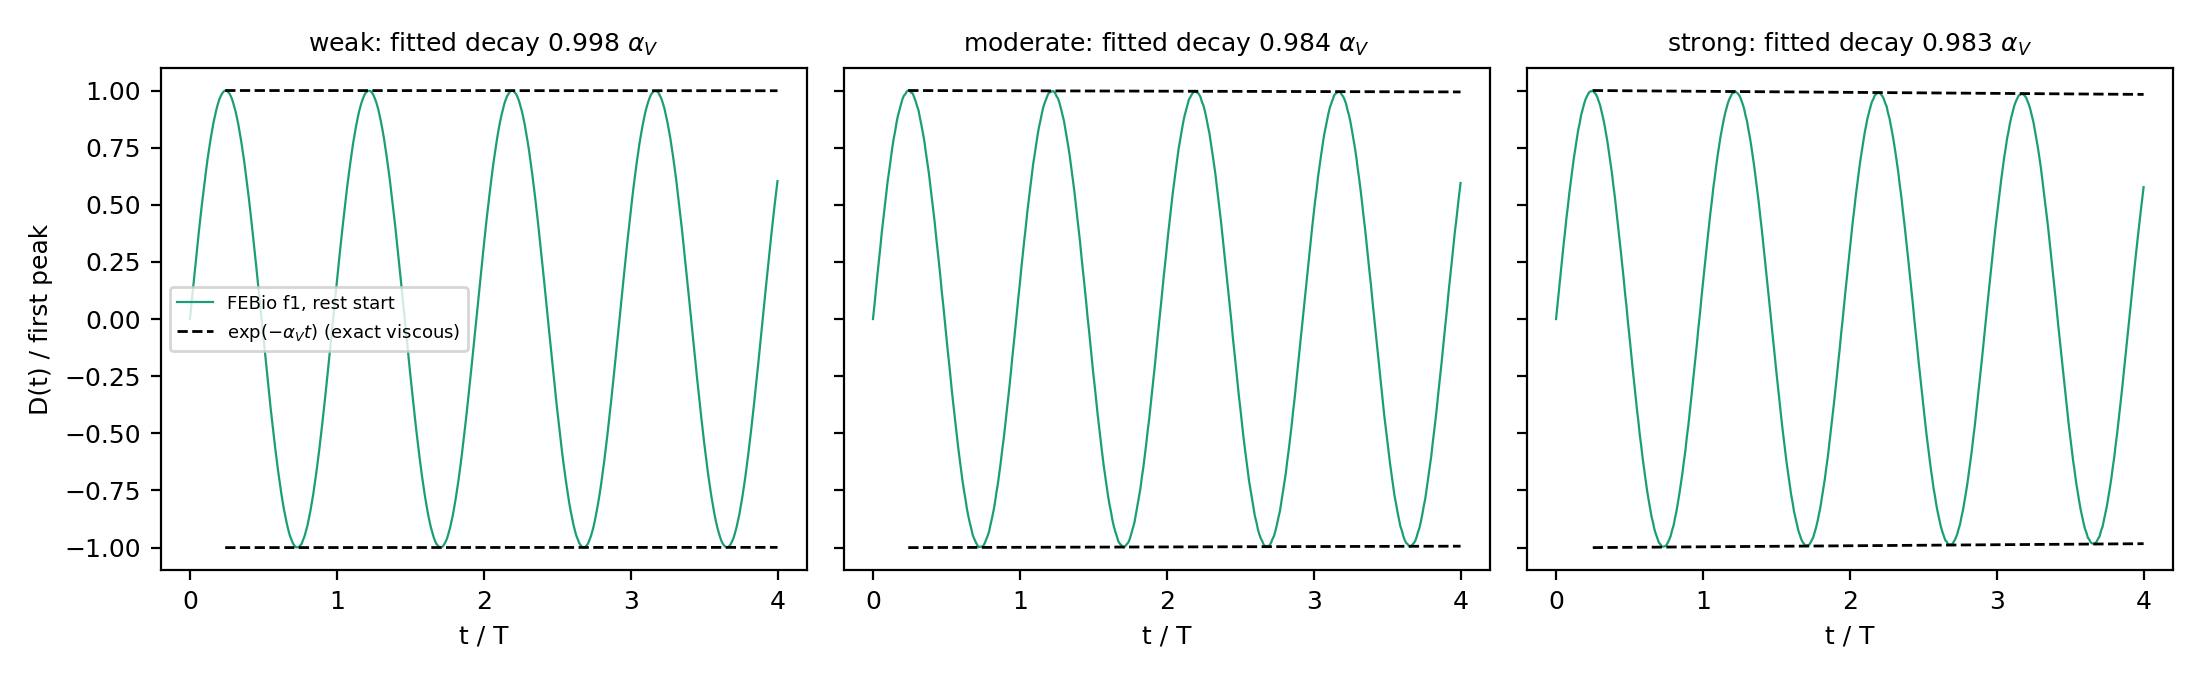
\includegraphics[width=\textwidth]{figures/verification/ringAddedMass_febio_R3}
	\caption{ringAddedMass, FEBio displacement histories $D=(u_r(0^\circ)-u_r(90^\circ))/2$ at the f1 resolution with the fluid at rest, normalised by the first peak, for the weak, moderate and strong levels, with the exact viscous envelope $\exp(-\alpha_V t)$. The fitted decay rates are $0.998$, $0.984$ and $0.983$ times $\alpha_V$.}
	\label{fig:ring_febio_decay}
\end{figure}

\emph{Interface mechanics.}
The pressure and viscous traction that FEBio's fluid--FSI surface load applies to the ring were reconstructed from logged nodal dilatation and element stress (Figure~\ref{fig:ring_febio_traction}).
The work of the reconstructed traction equals the ring's kinetic plus strain energy change to $0.02$--$0.09\%$ of the energy swing ($1.9\%$ for the strong level started at rest), which checks the orientation, the area measure and the sign independently of the force magnitude, and the $n=2$ viscous shear amplitude is $0.84$--$0.90$ of the thin-Stokes-layer estimate computed from the logged velocities, with a shear-to-pressure traction ratio of $4\times10^{-4}$ to $8\times10^{-4}$.
For the strong level started from the potential-flow field, the energy lost by the fluid including the integrated viscous dissipation balances the work on the ring to $0.5\%$ of the ring's energy swing, and the discrete energy balance is closed to $0.3\%$ of the initial energy.
These are reconstructions and one-element-gradient dissipation estimates, not measured interface forces; the weak level started from the potential-flow field did not converge in its first step and is not reported.
\begin{figure}[htbp]
	\centering
	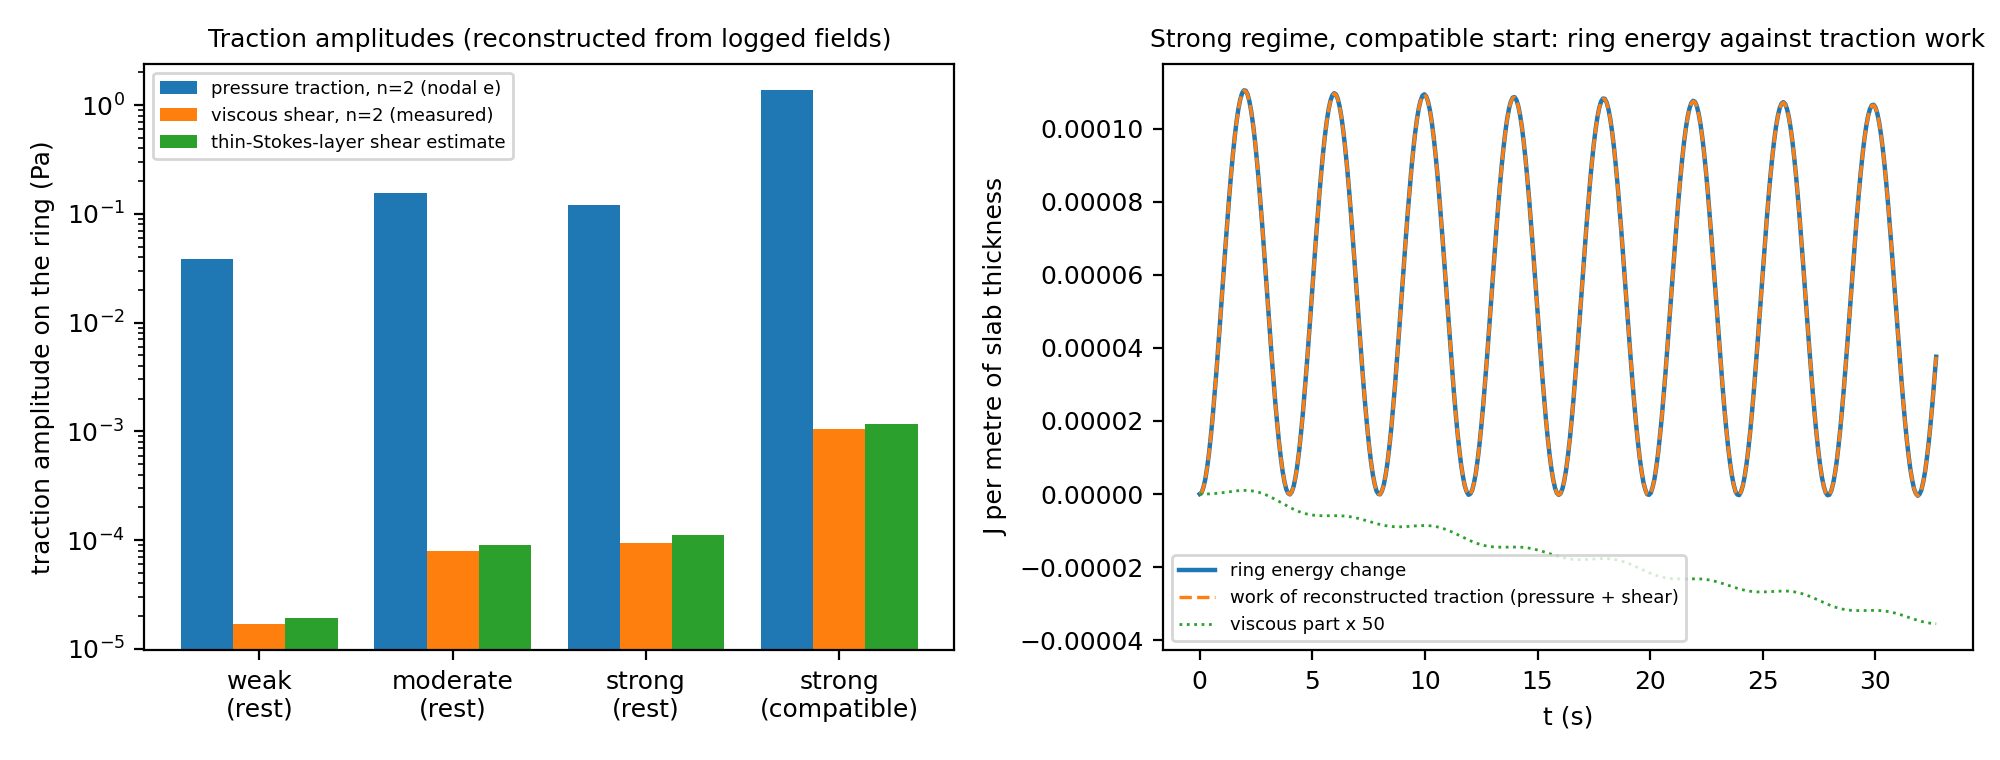
\includegraphics[width=\textwidth]{figures/verification/ringAddedMass_febio_R4}
	\caption{ringAddedMass, FEBio interface traction on the ring, reconstructed from logged fields. Left: $n=2$ amplitudes of the pressure traction, the viscous shear traction and the thin-Stokes-layer shear estimate (fluid at rest, and the strong level from the potential-flow field). Right: strong level, potential-flow start, the ring's energy change and the work of the reconstructed traction (the viscous part, multiplied by 50, is dissipative). Source: \texttt{paper-data/febio\_ring\_added\_mass/no\_slip\_resolved/}.}
	\label{fig:ring_febio_traction}
\end{figure}



\fi

\end{appendices}


\bibliography{bibliography}% common bib file


\end{document}
